% !TeX root = ../../Book1.tex
% 纲要标题：## 第15章　联络、曲率与平行移动
% 纲要位置：几何学计划纲要.md，第 690 行。
% 正文状态：初稿；尚未正式审核。

% 纲要内容开始
% 
% > 本章目标与证明范围：从“不同点的向量如何比较”构造联络，再以曲率测量路径依赖。完整证明局部公式、变换律、Bianchi 和平坦局部模型；不把曲率只写成一个矩阵公式。
% 
% 纲要内容结束

\chapter{联络、曲率与平行移动}
\label{g1:ch:15}
\BookChapterNumber{g1:ch:15}

\begin{chapterabstract}
	不同点的纤维没有默认的比较方式，联络为这种比较提供一阶规则。我们先从 Leibniz 法则构造局部联络矩阵，证明整体存在、换标架规律与仿射空间结构，再把联络化为沿路径的线性常微分方程。平行移动反过来恢复协变导数，并把度量相容解释成长度保持。曲率由两次协变微分的不交换性产生，其结构方程和小环路展开连接局部计算与实际运输；Bianchi 恒等式表达这些变化之间的相容关系。对切丛，还能用 Lie 括号定义挠率，区分平行标架与坐标标架。最后由平坦方程逐方向构造平行标架，用连续同伦的网格论证证明路径无关性，并由基本群表示记录仍可能存在的整体单值。
\end{chapterabstract}

\begin{learninggoals}
	\begin{itemize}
		\item 理解联络两个输入的不同线性要求，证明局部矩阵公式、整体存在及两联络之差的张量性，构造对偶与张量上的诱导联络。
		\item 完整建立沿路径的平行移动，掌握拼接、反向、参数依赖和恢复联络的公式，并证明度量相容与运输保长等价。
		\item 证明曲率的张量性、结构方程及换标架共轭规律，用小环路计算解释曲率，并推导 Bianchi 恒等式。
		\item 构造切丛联络的挠率，推导第一结构方程，区分无挠性、平坦性和度量相容性，判断平行标架何时可由坐标实现。
		\item 从曲率为零构造局部平行标架，证明平坦运输的同伦不变性与单连通区域上的路径无关性，用单值表示解释整体障碍。
	\end{itemize}
\end{learninggoals}

在 Euclid 空间中，我们习惯把两个不同点的向量平移到一起相减。第八、九章已经提醒我们：曲面的切向量属于不同切平面，必须先说明如何比较，才谈得上“方向没有改变”。第十二章将这种情形推广到一般向量丛，第十四章又建立了不依赖坐标的微分形式运算。现在要把这两条线连接起来：既允许纤维随点变化，又保留微分的乘法法则。

\ProseParagraphBreak

局部标架能暂时把邻近纤维认作同一个向量空间，但这种认法随标架选择而变。联络矩阵补偿标架的变化；沿路径解相应方程，便得到由联络指定的比较。两条路径的比较结果不一致时，局部的小环路由曲率控制，较大的绕行还可能涉及基本群。圆周上的例子将展示曲率处处为零、绕行运输仍非平凡的联络，从而把局部曲率与整体单值分开。

\ProseParagraphBreak

本章默认底流形有限维、Hausdorff、第二可数，向量丛为有限秩实光滑丛；除明确限于内点的坐标实现及小方环计算外，允许流形有边界。需要的前置工具是\chapref{g1:ch:12}的局部标架、张量构造和单位分解，\secref{g1:sec:1301}的常微分方程存在唯一性与参数依赖，以及\chapref{g1:ch:14}的外微分和局部恰当性。\secref{g1:sec:1505}还会回顾\chapref{g1:ch:05}的路径同伦、基本群与覆盖。调用时均重申具体条件，不要求读者记住前章每个技术细节。

\ProseParagraphBreak

本章的联络构造、局部公式、运输、曲率恒等式与平坦局部模型均在正文证明。延伸阅读可查 Tu 的第一版：第6.2节 的 Torsion and Curvature，第10--11节 的向量丛联络、存在性及联络、曲率、挠率形式，第13.1节 的 Covariant Differentiation Along a Curve，以及 第14.5--14.7节 的 Parallel Translation 及其存在性、度量情形\cite[第6.2、10--11、13.1、14.5--14.7节]{Tu2017Connections}。本书继续使用行标架 \(e\)、列分量 \(u\)、\(\nabla(eu)=e(\mathrm{d}u+Au)\) 的约定；对读其他文献时，应先核对矩阵放在哪一侧，再比较符号。

% !TeX root = ../../Book1.tex
% 纲要标题：### 15.1 丛联络及其空间
% 纲要位置：几何学计划纲要.md，第 694 行。
% 正文状态：初稿；尚未正式审核。

% 纲要内容开始
% 
% * Leibniz 规则与局部联络矩阵
% * 联络的整体存在
% * 两联络之差与仿射空间结构
% * 对偶、张量及外幂上的诱导联络
% 
% 纲要内容结束

\section{丛联络及其空间}
\label{g1:sec:1501}

一个截面 \(s\) 在不同点取值于不同纤维，所以表达式 \(s(q)-s(p)\) 通常没有意义。局部标架能把这些值写成同一个 \(\mathbb R^r\) 中的列向量，于是可以对分量求导；然而标架自己也可能随基点变化，只对分量求导会依赖这次选择。曲面上的协变导数曾用“先在环境空间求导，再投影回切空间”处理这一问题。一般向量丛未指定环境空间，我们需要直接规定一种微分运算，使它在换标架后仍表示同一个几何对象。

\ProseParagraphBreak

本节讨论有限秩实光滑向量丛 \(E\to M\)，其中 \(M\) 有限维、Hausdorff、第二可数，允许有边界。局部平凡化和截面沿用第12章的定义：标架写成行 \(e=(e_1,\ldots,e_r)\)，截面写成 \(s=e u\)，其中 \(u\) 是列分量。边界处的光滑函数与截面均按局部延拓定义；联络作用于完整的切空间，不要求求导方向切于边界。

\subsection{Leibniz 规则与局部联络矩阵}
\label{g1:subsec:1501:01}

对函数倍乘的截面 \(fs\) 求导时，一部分变化来自 \(f\)，另一部分来自 \(s\)。前一部分应当仍由普通方向导数 \(Xf\) 描述。这个要求给出联络的乘积法则。方向 \(X\) 则只指定在哪个切向量上求导，不应再对 \(X\) 的系数求导；因此两个输入承担不同的线性条件。

\begin{definition}[丛联络]\label{g1:def:bundle-connection}
	设 \(M\) 为有限维、Hausdorff、第二可数光滑流形，允许有边界，\(E\to M\) 为有限秩实光滑向量丛。一个实双线性映射
	\[
		\nabla:\mathfrak X(M)\times\Gamma(E)\longrightarrow\Gamma(E),\qquad (X,s)\longmapsto\nabla_Xs,
	\]
	若对每个 \(f\in C^\infty(M)\) 满足
	\[
		\nabla_{fX}s=f\nabla_Xs,\qquad
		\nabla_X(fs)=X(f)s+f\nabla_Xs,
	\]
	就称为 \(E\) 上的\term[conglianluo]{丛联络}[vector bundle connection]，简称联络。\(\nabla_Xs\) 称为 \(s\) 沿 \(X\) 的协变导数。这里的丛联络都是线性联络，即遵守所写的实线性条件。
\end{definition}

第一个公式是对方向输入的 \(C^\infty(M)\) 线性，第二个公式是对截面输入的 Leibniz 规则，不能交换二者的职责。例如在平凡实线丛 \(M\times\mathbb R\) 的标准标架 \(e\) 中，\(\nabla_X(fe)=X(f)e\) 就满足定义。若把第二个输入也要求成 \(C^\infty(M)\) 线性，便会删掉函数本身的变化，无法包含这个最基本的例子。

\begin{proposition}[联络的局部性]\label{g1:prop:connection-locality}
	设 \(M\) 为有限维、Hausdorff、第二可数光滑流形，允许有边界，\(E\to M\) 为有限秩实光滑向量丛，\(\nabla\) 为其联络。则有以下结论。
	\begin{enumerate}
		\item \(\nabla_Xs\) 在开集 \(U\) 上的限制，只依赖 \(X,s\) 在 \(U\) 上的限制。因此 \(\nabla\) 唯一地作用于任意开集上的局部向量场和局部截面，并满足相同的线性与乘积规则。
		\item 对 \(p\in M\)，\((\nabla_Xs)(p)\) 对方向场只依赖 \(X_p\)。给定任意 \(v\in \mathrm{T}_pM\) 及 \(p\) 附近的局部截面 \(s\)，可以良定义
		\[
			\nabla_v s\coloneqq(\nabla_Xs)(p),\qquad X_p=v.
		\]
		它属于 \(E_p\)，且对 \(v\) 实线性。
	\end{enumerate}
\end{proposition}
\begin{proof}
	先设整体截面 \(s\) 在 \(p\) 的开邻域 \(U\) 中为零。由\cref{g1:cor:smooth-cutoff-closed}，可取在 \(p\) 附近等于 \(1\)、支集紧且包含于 \(U\) 的光滑函数 \(\chi\)。因为 \(\chi s=0\)，Leibniz 规则给出
	\[
		0=\nabla_X(\chi s)=X(\chi)s+\chi\nabla_Xs.
	\]
	在 \(\chi=1\) 的邻域中，\(X(\chi)=0\)，所以 \(\nabla_Xs=0\)。若整体向量场 \(X\) 在 \(U\) 上为零，则 \(\chi X=0\)，由方向输入的函数线性得到 \(0=\nabla_{\chi X}s=\chi\nabla_Xs\)，结论相同。作差便知局部相同的输入给出局部相同的输出。

	现设 \(X,s\) 只在 \(U\) 上定义。对每个 \(p\in U\) 选上述 \(\chi\)，将 \(\chi X,\chi s\) 在 \(U\) 外补零。所得整体场和截面光滑：在 \(U\) 内按乘法光滑，在 \(U\) 外每点附近因支集包含于 \(U\) 而恒为零。用整体联络求导后，在 \(\chi=1\) 的邻域内作为局部定义。不同截断或延拓在较小邻域中相同，刚证明的局部性保证结果也相同，故各点的结果粘合为 \(U\) 上的光滑截面。对局部函数同样用截断延拓，便能从整体规则得到局部规则。唯一性来自每点附近都可以这样替换成整体输入。

	最后，在 \(p\) 附近取坐标 \(x^1,\ldots,x^n\)，写 \(X=\sum_iX^i\partial_i\)。已建立的局部规则给出
	\[
		(\nabla_Xs)(p)=\sum_iX^i(p)(\nabla_{\partial_i}s)(p).
	\]
	因此 \(X_p=0\) 时输出为零，两个方向场在 \(p\) 相同时也给出相同值。任意 \(v=\sum_iv^i\partial_i|_p\) 可以由局部常分量场 \(\sum_iv^i\partial_i\) 实现，再乘紧支截断延成整体场，故所有切向量都能作为输入。边界图的坐标向量仍构成完整的 \(n\) 维切空间基，这一构造没有使用保持 \(M\) 的流，也没有限制 \(v\) 的法向分量。线性直接由公式得到。
\end{proof}

点处求值的两个输入仍不对称。\(\nabla_v s\) 可以只记方向向量 \(v\)，却通常不能只记纤维向量 \(s(p)\)。例如在 \(\mathbb R\) 上的平凡线丛中，标准联络使截面 \(s(x)=xe\) 满足 \(s(0)=0\)、\(\nabla_{\partial_x|_0}s=e\)，而零截面有相同的点值，导数却为零。因此联络并没有给每个 \(v\) 一个可直接作用于 \(E_p\) 的线性自同态；它还需要知道截面在附近如何变化。

\begin{definition}\label{g1:def:bundle-valued-form}
	设 \(M\) 为有限维、Hausdorff、第二可数光滑流形，允许有边界，\(E\to M\) 为有限秩实光滑向量丛。记
	\[
		\Omega^k(M;E)\coloneqq\Gamma(\Lambda^k\mathrm{T}^*M\otimes E),\qquad k\geq0,
	\]
	其元素称为 \(E\) 值微分形式，也称\term[congzhiweifenxingshi]{丛值微分形式}[bundle-valued differential form]，\(\Omega^0(M;E)=\Gamma(E)\)。\symidx{\(\Omega^k(M;E)\)：丛值微分形式空间}对 \(k=1\)，它在每个点是从 \(\mathrm{T}_pM\) 到 \(E_p\) 的线性映射，随基点光滑变化。
\end{definition}

这里的丛已由\cref{g1:prop:tensor-bundle-constructions}构造，\(\mathrm{T}_p^*M\otimes E_p\simeq\operatorname{Hom}(\mathrm{T}_pM,E_p)\) 的识别来自\cref{g1:prop:tensor-hom-duality}及因子交换。固定截面 \(s\)，上一命题说明 \(v\mapsto\nabla_v s\) 给出一个 \(E\) 值一形式：在坐标中，它写成 \(\sum_i\mathrm{d}x^i\otimes\nabla_{\partial_i}s\)，所以光滑。记此一形式为 \(\nabla s\)，联络也就可以写成
\[
	\nabla:\Gamma(E)\longrightarrow\Omega^1(M;E),\qquad
	\nabla(fs)=\mathrm{d}f\otimes s+f\nabla s.
\]
反过来，一个满足此式的实线性映射通过 \(\nabla_Xs=(\nabla s)(X)\) 恢复定义中的两条规则。因此两种写法等价：前者突出求导方向，后者把各方向的结果放在同一个一形式中。

\ProseParagraphBreak

在局部标架 \(e=(e_1,\ldots,e_r)\) 中，各 \(\nabla e_b\) 是 \(E\) 值一形式，因而唯一写成 \(\nabla e_b=\sum_a A^a{}_b\otimes e_a\)。把一形式 \(A^a{}_b\) 排成矩阵 \(A\)，称为该标架中的\term[lianluojuzhen]{联络矩阵}[connection matrix]。为使行标架计算简洁，约定对一形式列 \(\eta\) 写 \(e\eta=\sum_a\eta^a\otimes e_a\)；于是 \(\nabla e=eA\) 表示刚才的逐列等式。它并没有改变 \(E\) 值形式中两个张量因子的类型。

\begin{proposition}[联络的局部表示]\label{g1:prop:connection-local-data}
	设 \(M\) 为有限维、Hausdorff、第二可数光滑流形，允许有边界，\(E\to M\) 为秩 \(r\) 的实光滑向量丛。联络 \(\nabla\) 在局部标架 \(e\) 中由一个 \(r\times r\) 的光滑一形式矩阵 \(A\) 唯一决定，具体为
	\begin{equation}
		\label{g1:eq:connection-local-form}
		\nabla e=eA,\qquad
		\nabla(eu)=e(\mathrm{d}u+A u),\qquad
		\nabla_X(eu)=e\bigl(X(u)+A(X)u\bigr).
	\end{equation}
	这里 \(\mathrm{d}u\) 与 \(X(u)\) 均逐分量计算。若换标架为 \(e'=eg\)，其中 \(g:U\to\operatorname{GL}(r,\mathbb R)\) 光滑，则新矩阵满足
	\begin{equation}
		\label{g1:eq:connection-frame-change}
		A'=g^{-1}Ag+g^{-1}\mathrm{d}g.
	\end{equation}
	反过来，若一个标架覆盖上的光滑一形式矩阵在交叠处满足此规律，则\eqref{g1:eq:connection-local-form}唯一地定义一个整体联络。
\end{proposition}
\begin{proof}
	把 \(s=\sum_bu^b e_b\) 代入 Leibniz 规则，得到
	\[
		\nabla s=\sum_b\mathrm{d}u^b\otimes e_b+\sum_{a,b}u^bA^a{}_b\otimes e_a
		=e(\mathrm{d}u+A u).
	\]
	对 \(X\) 求值便得到方向公式。反向，在一张有标架的开集上，任意光滑矩阵一形式 \(A\) 由此定义光滑输出；\(X(fu)=X(f)u+fX(u)\) 和 \(A(fX)=fA(X)\) 直接保证联络的两条规则。

	换标架时，逐列使用乘积法则可得
	\[
		\nabla e'=\nabla(eg)=e(Ag+\mathrm{d}g)=e'g^{-1}(Ag+\mathrm{d}g).
	\]
	由于 \(\nabla e'=e'A'\)，这就是\eqref{g1:eq:connection-frame-change}。同一截面的分量满足 \(u=gu'\)，于是该规律还给出
	\[
		e'(\mathrm{d}u'+A'u')
		=e\bigl(g\,\mathrm{d}u'+\mathrm{d}g\,u'+Ag u'\bigr)
		=e\bigl(\mathrm{d}(gu')+A(gu')\bigr).
	\]
	因此满足变换规律的局部矩阵对同一截面给出相同的一形式，能够逐点粘合。光滑性和联络规则都是局部性质，故粘合结果是整体联络；各张图中的公式又完全确定它，所以唯一。边界图中的微分按局部光滑延拓计算，\cref{g1:prop:boundary-smooth-derivative}保证链式法则及所得导数不依赖延拓，上述论证同样成立。
\end{proof}

若原来采用第12章的记号 \(e_j=e_i g_{ij}\)，这里的公式就是 \(A_j=g_{ij}^{-1}A_i g_{ij}+g_{ij}^{-1}\mathrm{d}g_{ij}\)。注意它含有 \(g\) 的导数。联络矩阵不是一个单纯按共轭变换的张量，\(A=0\) 也不是换标架后保持不变的断言。

\begin{example}
	在平凡实线丛中，令标准标架 \(e\) 下的联络为 \(\nabla(fe)=\mathrm{d}f\otimes e\)，于是 \(A=0\)。取另一标架 \(e'=e e^h\)，其中 \(h\) 是任意光滑实函数，则 \(g=e^h\)，从而
	\[
		A'=e^{-h}\mathrm{d}(e^h)=\mathrm{d}h.
	\]
	同一截面 \(fe\) 在新标架中的分量为 \(u'=e^{-h}f\)。因此
	\[
		e'\bigl(\mathrm{d}(e^{-h}f)+(\mathrm{d}h)e^{-h}f\bigr)=e\,\mathrm{d}f.
	\]
	对分量求导时出现的额外项，恰被联络矩阵抵消。新标架中的矩阵非零，并不表示我们更换了联络。
\end{example}

\subsection{联络的整体存在}
\label{g1:subsec:1501:02}

在一张平凡化中，把联络矩阵取为零就得到联络。困难在于不同平凡化的“零矩阵”一般不满足变换公式，所以不能直接宣称它们粘成整体对象。单位分解提供另一种做法：先把各个局部联络的输出乘以权重，再相加。Leibniz 规则中需要保留的普通导数项，正好由权重之和等于 \(1\) 来保证。

\begin{theorem}[联络的存在]\label{g1:thm:connection-existence}
	设 \(M\) 为有限维、Hausdorff、第二可数光滑流形，允许有边界，\(E\to M\) 为有限秩实光滑向量丛。则 \(E\) 上存在光滑联络。
\end{theorem}
\begin{proof}
	取局部标架覆盖 \(\{U_i,e_i\}\)，在每个 \(U_i\) 上令
	\[
		\nabla^{(i)}(e_i u)=e_i\,\mathrm{d}u.
	\]
	这是局部联络。由\cref{g1:thm:smooth-partition-unity}，存在从属于 \(\{U_i\}\) 的光滑单位分解 \(\{\rho_i\}\)，满足支集族局部有限、\(\operatorname{supp}\rho_i\subseteq U_i\) 及 \(\sum_i\rho_i=1\)。对整体截面 \(s\)，定义
	\[
		\nabla s=\sum_i\rho_i\nabla^{(i)}(s|_{U_i}),
	\]
	其中每项在 \(U_i\) 外补零。这样的补零光滑：任何 \(U_i\) 外的点都有一个避开闭集 \(\operatorname{supp}\rho_i\) 的邻域，在此邻域该项恒为零。每点附近只有有限个非零项，所以和是光滑的 \(E\) 值一形式，且对 \(s\) 实线性。

	对 \(f\in C^\infty(M)\)，在每个点的有限求和邻域内，有
	\begin{align*}
		\nabla(fs)
		&=\sum_i\rho_i\bigl(\mathrm{d}f\otimes s+f\nabla^{(i)}s\bigr)\\
		&=\left(\sum_i\rho_i\right)\mathrm{d}f\otimes s+f\sum_i\rho_i\nabla^{(i)}s
		=\mathrm{d}f\otimes s+f\nabla s.
	\end{align*}
	于是按一形式对方向求值，就得到所需联络。证明使用的局部标架与单位分解在带边界流形上也存在，故包含边界情形。秩零时所有截面和输出均为零，结论也成立。
\end{proof}

支集包含于 \(U_i\) 与局部有限性各自有明确作用：前者使局部输出能够光滑补零，后者使求和、求导都成为邻域内的有限运算。权重在此乘在联络的输出上，验证乘积法则时不对 \(\rho_i\) 求导。构造依赖所选局部标架与单位分解，存在定理没有给出一个由向量丛本身唯一指定的联络。

\begin{example}
	Möbius 实线丛的局部过渡函数可以取为 \(1\) 或 \(-1\)，在每个交叠连通分支上为常数，见\cref{g1:exm:mobius-line-bundle}。因此 \(\mathrm{d}g_{ij}=0\)，在这些局部标架中同时取 \(A_i=0\) 就满足联络变换公式，直接给出整体联络。这个丛没有全局处处非零截面，却仍有联络。由此可见，给出一种相容的求导规则，并不等于给出一个全局标架。
\end{example}

\subsection{两联络之差与仿射空间结构}
\label{g1:subsec:1501:03}

单个联络对截面求导时包含函数的一阶变化。若对同一个截面使用两个联络，再把结果相减，普通微分项就会消掉。留下的运算只观察该截面在一点的值，因而成为真正的张量。这也解释了为什么联络的矩阵变换带一个附加项，而两个矩阵的差没有。

\begin{proposition}[联络的仿射空间]\label{g1:prop:connection-affine-space}
	设 \(M\) 为有限维、Hausdorff、第二可数光滑流形，允许有边界，\(E\to M\) 为有限秩实光滑向量丛。两个联络 \(\nabla^0,\nabla^1\) 唯一确定
	\[
		B\in\Omega^1(M;\operatorname{End}E)
	\]
	使
	\[
		\nabla^1_Xs-\nabla^0_Xs=B(X)s
	\]
	对所有 \(X,s\) 成立。反过来，给定联络 \(\nabla\) 和任意这样的 \(B\)，公式 \((\nabla+B)_Xs=\nabla_Xs+B(X)s\) 定义一个联络。因此全部联络的集合 \(\operatorname{Conn}(E)\) 是以 \(\Omega^1(M;\operatorname{End}E)\) 为方向空间的非空仿射空间。\symidx{\(\operatorname{Conn}(E)\)：联络的仿射空间}
\end{proposition}
\begin{proof}
	令 \(D(X,s)=\nabla^1_Xs-\nabla^0_Xs\)。方向输入的函数线性由两个联络的相同性质得到；对截面输入，Leibniz 项相消，故
	\[
		D(fX,s)=fD(X,s),\qquad D(X,fs)=fD(X,s).
	\]
	先前的局部性保证 \(D\) 可作用于局部输入。在 \(p\) 附近取坐标及标架，写 \(X=\sum_iX^i\partial_i\)、\(s=\sum_a u^a e_a\)，便有
	\[
		D(X,s)(p)=\sum_{i,a}X^i(p)u^a(p)D(\partial_i,e_a)(p).
	\]
	右端只依赖 \(X_p\) 与 \(s(p)\)，并且对二者实双线性。任何 \(v\in \mathrm{T}_pM\)、\(w\in E_p\) 都能由局部常分量场及截面实现，再用紧支截断延成整体输入。因此定义 \(B_p(v)w=D(X,s)(p)\) 与选择无关，也唯一。

	各 \(D(\partial_i,e_a)\) 光滑，所以上式同时给出 \(B\) 的光滑局部系数，得到 \(B\in\Gamma(\mathrm{T}^*M\otimes\operatorname{End}E)\)。在一组标架中若两个联络矩阵为 \(A^0,A^1\)，则 \(B\) 的矩阵一形式就是 \(A^1-A^0\)。由\eqref{g1:eq:connection-frame-change}，换标架后
	\[
		B'=g^{-1}Bg,
	\]
	因为两个 \(g^{-1}\mathrm{d}g\) 项消掉了。这正是自同态值一形式所应有的变换规律。

	反向，\(B(X)s\) 对两个输入都为函数线性，因此将它加到联络上，方向线性不变，对截面的乘积法则仍只有原来的 \(X(f)s\) 项。故 \(\nabla+B\) 是联络。存在定理保证联络集合非空；上面的差与加法互相对应，满足
	\[
		(\nabla+B)+C=\nabla+(B+C),\qquad \nabla+0=\nabla,
	\]
	而任意两个联络之间有且只有一个 \(B\) 把前者移到后者。这就是仿射空间的加法公理，不要求方向空间有限维。
\end{proof}

选择一个参考联络 \(\nabla^0\) 后，任何联络都唯一写成 \(\nabla^0+B\)，从而可用向量空间 \(\Omega^1(M;\operatorname{End}E)\) 参数化。但参考联络是一个选择；更换它会平移全部参数。尤其不能把矩阵 \(A=0\) 当成与标架无关的“零联络”。在正维流形上的正秩丛中，零算子一般连 Leibniz 规则都不满足：它会把 \(\nabla_X(fs)\) 置为零，却遗漏可能非零的 \(X(f)s\)。

\ProseParagraphBreak

仿射组合则没有这一问题。如果 \(\nabla^0,\ldots,\nabla^m\) 是联络，光滑函数 \(f_0,\ldots,f_m\) 满足 \(\sum_j f_j=1\)，那么 \(\sum_j f_j\nabla^j\) 仍是联络，证明与存在定理中的乘积法则计算相同；此处不要求 \(f_j\) 非负。特别地，\((1-t)\nabla^0+t\nabla^1\) 对每个实数 \(t\) 都是联络。若 \(\dim M=0\) 或 \(\operatorname{rank}E=0\)，方向空间为零，联络只有一个，这与仿射描述也相容。

\subsection{对偶、张量及外幂上的诱导联络}
\label{g1:subsec:1501:04}

给 \(E\) 选择求导规则之后，它的对偶与张量构造不应再独立任选一套规则。例如 \(\lambda\in\Gamma(E^*)\) 与 \(s\in\Gamma(E)\) 配对得到普通函数 \(\lambda(s)\)；若对它求导，结果应与先分别求导再配对一致。这个要求决定了对偶联络的负号。张量积和外幂则应沿每个因子分别求导，再把结果相加。

\begin{proposition}[诱导联络]\label{g1:prop:induced-connections}
	设 \(M\) 为有限维、Hausdorff、第二可数光滑流形，允许有边界，\(E,F\to M\) 为有限秩实光滑向量丛，分别给定联络 \(\nabla^E,\nabla^F\)。存在以下唯一的诱导联络。
	\begin{enumerate}
		\item 对偶丛 \(E^*\) 上的联络满足
		\[
			X\bigl(\lambda(s)\bigr)=(\nabla^{E^*}_X\lambda)(s)+\lambda(\nabla^E_Xs),
			\qquad \lambda\in\Gamma(E^*),\ s\in\Gamma(E).
		\]
		\item 张量积丛 \(E\otimes F\) 上的联络满足
		\[
			\nabla^{E\otimes F}_X(s\otimes t)
			=(\nabla^E_Xs)\otimes t+s\otimes\nabla^F_Xt.
		\]
		重复此构造得到任意有限个张量因子上的联络；它与因子的排列及对偶求值产生的收缩相容。
		\item 对每个整数 \(k\geq1\)，外幂 \(\Lambda^kE\) 上的联络满足
		\[
			\nabla^{\Lambda^kE}_X(s_1\wedge\cdots\wedge s_k)
			=\sum_{j=1}^k s_1\wedge\cdots\wedge\nabla^E_Xs_j\wedge\cdots\wedge s_k.
		\]
		零次外幂是平凡实线丛，其诱导联络为 \(\nabla_Xf=Xf\)。对称幂上有把 \(\wedge\) 换成 \(\odot\) 的同类公式。
		\item 同态丛 \(\operatorname{Hom}(E,F)\) 上的联络满足
		\[
			(\nabla^{\operatorname{Hom}}_X\mathcal B)(s)
			=\nabla^F_X(\mathcal B s)-\mathcal B(\nabla^E_Xs),
			\qquad \mathcal B\in\Gamma(\operatorname{Hom}(E,F)).
		\]
	\end{enumerate}
\end{proposition}
\begin{proof}
	先构造对偶联络。给定 \(X,\lambda\)，令
	\[
		Q(s)=X\bigl(\lambda(s)\bigr)-\lambda(\nabla^E_Xs).
	\]
	若把 \(s\) 换成 \(fs\)，第一项中的 \(X(f)\lambda(s)\) 与第二项中的相同项相消，故 \(Q(fs)=fQ(s)\)。所以 \(Q\) 在一点处只依赖 \(s\) 在该点的值：可以先用紧支截断把局部截面延拓，再展开为局部标架的函数组合，得到 \(Q(s)(p)=\sum_a u^a(p)Q(e_a)(p)\)。这与\cref{g1:prop:connection-locality}中的局部化论证相同，所需的函数线性刚刚已经验证。于是 \(Q\) 唯一确定一个对偶截面，规定为 \(\nabla^{E^*}_X\lambda\)。

	它的光滑性和具体符号也可直接看出。令 \(\lambda=\sum_a\ell_a e^a\)，其中 \((e^a)\) 为 \((e_a)\) 的对偶标架，\(\ell\) 为列分量。若 \(\nabla^E\) 的矩阵为 \(A\)，对 \(s=e u\) 展开上式得到
	\[
		Q(s)=X(\ell^{\mathsf T}u)-\ell^{\mathsf T}\bigl(X(u)+A(X)u\bigr)
		=\bigl(X(\ell)-A(X)^{\mathsf T}\ell\bigr)^{\mathsf T}u.
	\]
	所以对偶联络的列分量为 \(\mathrm{d}\ell-A^{\mathsf T}\ell\)，对偶标架中的联络矩阵为 \(-A^{\mathsf T}\)。它对方向输入函数线性；把 \(\lambda\) 换成 \(f\lambda\)，公式给出 \(\nabla^{E^*}_X(f\lambda)=X(f)\lambda+f\nabla^{E^*}_X\lambda\)。故它确实为联络。求值恒等式不依赖标架，所以各图中的构造相容，且该恒等式决定了它在每个纤维向量上的值，保证唯一。

	再构造张量积联络。在局部标架 \((e_a)\)、\((h_b)\) 中，\(e_a\otimes h_b\) 构成 \(E\otimes F\) 的标架，见\cref{g1:thm:tensor-product-universal,g1:prop:tensor-bundle-constructions}。先规定
	\[
		\nabla_X(e_a\otimes h_b)
		=(\nabla^E_Xe_a)\otimes h_b+e_a\otimes\nabla^F_Xh_b,
	\]
	再对一般截面 \(w=\sum_{a,b}w^{ab}e_a\otimes h_b\) 按 \(X(w^{ab})\) 和 Leibniz 规则定义。基展开唯一，所以得到一个良定义的局部联络。把 \(s=\sum_a s^a e_a\)、\(t=\sum_b t^b h_b\) 代入，普通乘积法则 \(X(s^at^b)=X(s^a)t^b+s^aX(t^b)\) 正好给出命题所述纯张量公式。特别地，在 \((fs)\otimes t=s\otimes(ft)\) 的两种写法中，额外的 \(X(f)s\otimes t\) 项相同，不会产生不同结果。

	任取另一组标架，它的每个张量基元素仍是两个局部截面的纯张量，故刚构造的联络也满足该组基上的同一规定。再用对系数的 Leibniz 规则，得到两组构造在任意截面上相同，因而能够整体粘合。纯张量基上的规定也证明唯一性。多个张量因子时，重复同一构造得到“对每个位置求导后相加”的公式。改变括号或排列因子，只会重新排列这组求和项，所以与这些自然识别相容。

	收缩的相容性来自对偶公式。对纯张量中一对因子 \(\lambda,s\) 作收缩时，它们被替换成函数 \(\lambda(s)\)。对这一函数求导产生的两个项，正好是先对 \(\lambda\) 或 \(s\) 求导再收缩的结果；其余因子上的求导项保持不变。纯张量局部张成全部张量，故一般收缩也与诱导联络相容。

	接下来说明外幂公式确实尊重外幂的关系，而不仅是在可分解元素上写出一个表达。对 \(E^{\otimes k}\)，记 \(P_\sigma\) 为按置换 \(\sigma\) 重新排列因子的光滑丛映射，定义交替化算子
	\[
		\operatorname{Alt}=\frac1{k!}\sum_{\sigma\in S_k}\operatorname{sgn}(\sigma)P_\sigma.
	\]
	\(\operatorname{Alt}^2=\operatorname{Alt}\)：在两次求和中，每个合成置换恰出现 \(k!\) 次，符号相乘等于合成的符号。若纯张量有两个相同因子，按交换这两个位置把求和项配对，便知其交替化为零。因此 \(\operatorname{Alt}\) 消去\cref{g1:def:symmetric-exterior-powers}中定义外幂的关系子空间，诱导出 \(\Lambda^kE\to\operatorname{im}(\operatorname{Alt})\)。

	设 \(q:E^{\otimes k}\to\Lambda^kE\) 为自然商映射。交换输入改变楔积符号，所以 \(qP_\sigma=\operatorname{sgn}(\sigma)q\)，进而 \(q\operatorname{Alt}=q\)。因此刚才的诱导映射与 \(q\) 限制在 \(\operatorname{im}(\operatorname{Alt})\) 上的映射互逆：一个方向由 \(q\operatorname{Alt}=q\) 给出，另一方向由 \(\operatorname{Alt}^2=\operatorname{Alt}\) 给出。这些映射在张量标架中都是固定的有限线性组合，故为光滑识别。

	张量积联络与每个 \(P_\sigma\) 相容，因而与 \(\operatorname{Alt}\) 相容。若 \(w=\operatorname{Alt}w\)，则 \(\nabla_Xw=\operatorname{Alt}(\nabla_Xw)\)，所以它保持交替化像中的截面。通过上述识别，将此联络传到 \(\Lambda^kE\)，就得到外幂联络。对 \(q(s_1\otimes\cdots\otimes s_k)\) 使用张量求导公式，恰得到所述楔积公式。递增指标楔积构成局部标架，见\cref{g1:prop:symmetric-exterior-bases}，故该公式也保证唯一性。\(k>\operatorname{rank}E\) 时外幂为零丛，结论仍成立。\(k=0\) 按普通函数求导，\(k=1\) 则恢复原联络。去掉交替化中的符号得到对称化平均；它消去排列之差，且与张量联络相容，同一论证便给出对称幂上的联络。

	最后，\cref{g1:prop:tensor-hom-duality}给出 \(\operatorname{Hom}(E,F)\simeq F\otimes E^*\)，故已有一个张量诱导联络。对纯张量 \(\mathcal B=t\otimes\lambda\)，其作用为 \(\mathcal B s=\lambda(s)t\)，于是
	\begin{align*}
		\nabla^F_X(\mathcal B s)-\mathcal B(\nabla^E_Xs)
		&=X(\lambda(s))t+\lambda(s)\nabla^F_Xt-\lambda(\nabla^E_Xs)t\\
		&=(\nabla^{E^*}_X\lambda)(s)t+\lambda(s)\nabla^F_Xt\\
		&=\bigl(\nabla_X^{F\otimes E^*}(t\otimes\lambda)\bigr)(s).
	\end{align*}
	一般同态截面在每张图中是有限个这样的纯张量之和，所以上式对它也成立。求值于每个纤维向量能确定一个线性映射，故公式保证唯一性。以上所有构造只用了光滑系数、函数微分与有限次代数运算，边界处按局部延拓仍满足同样的公式。
\end{proof}

外幂联络在求导时保持外幂次数，因此
\[
	\nabla_X(\alpha\wedge\beta)=(\nabla_X\alpha)\wedge\beta+\alpha\wedge\nabla_X\beta
\]
没有外微分乘积法则中的 \((-1)^{\deg\alpha}\)。两种运算的类型不同：这里 \(\alpha,\beta\) 可以是 \(\Lambda^pE,\Lambda^qE\) 的截面，\(\nabla_X\) 在每个纤维的外代数上保持次数；第14章的 \(\mathrm{d}\) 作用于底流形的微分形式并使次数增加 \(1\)。即使取 \(E=\mathrm{T}^*M\)，也应保留这种区别。

\ProseParagraphBreak

诱导联络还给出了以后常用的求值公式。例如对光滑双线性形式场 \(h\in\Gamma(E^*\otimes E^*)\)，求导与收缩相容意味着
\begin{equation}
	\label{g1:eq:connection-bilinear-form}
	(\nabla_Xh)(s,t)=X\bigl(h(s,t)\bigr)-h(\nabla_Xs,t)-h(s,\nabla_Xt).
\end{equation}
这是先把 \(h,s,t\) 全部看作张量因子、对它们分别求导，再把 \(h\) 的导数移到等式一侧得到的。它同时记录了系数的变化与输入截面的变化，不能只保留第一项。

\ProseParagraphBreak

把同态联络写成矩阵，更能看清这种修正。在 \(E,F\) 的标架 \(e,h\) 中，设原联络矩阵分别为 \(A,C\)，同态截面 \(\mathcal B\) 由矩阵函数 \(B\) 表示，即 \(\mathcal B(eu)=hBu\)。对上面同态公式的右侧计算，有
\begin{align*}
	\nabla^F_X(\mathcal B(eu))&=h\bigl(X(B)u+B X(u)+C(X)Bu\bigr),\\
	\mathcal B(\nabla^E_X(eu))&=hB\bigl(X(u)+A(X)u\bigr).
\end{align*}
相减后含 \(X(u)\) 的项消去，说明结果确实只对输入向量的点值线性。同态值一形式 \(\nabla^{\operatorname{Hom}}\mathcal B\) 的矩阵因此为 \(\mathrm{d}B+CB-BA\)。当 \(F=E\)、两边使用同一个联络时，这成为
\begin{equation}
	\label{g1:eq:endomorphism-connection}
	(\nabla^{\operatorname{End}}\mathcal B)_e
	=\mathrm{d}B+[A,B],\qquad [A,B]=AB-BA.
\end{equation}
下标 \(e\) 表示取该自同态值一形式在标架 \(e\) 中的矩阵；\(B\) 是零次矩阵函数，故这里是通常的矩阵交换子，没有分次符号。

\ProseParagraphBreak

例如恒等自同态的矩阵为 \(I\)，所以 \(\nabla^{\operatorname{End}}\operatorname{id}_E=0\)。对两条自同态截面的复合，矩阵乘积法则给出
\[
	\mathrm{d}(BC)+A(BC)-(BC)A
	=(\mathrm{d}B+AB-BA)C+B(\mathrm{d}C+AC-CA).
\]
因此 \(\nabla_X^{\operatorname{End}}(\mathcal B\mathcal C)=(\nabla_X^{\operatorname{End}}\mathcal B)\mathcal C+\mathcal B\nabla_X^{\operatorname{End}}\mathcal C\)。对偶、张量和自同态上的这些规则使一个原始联络能够同时处理向量、线性观测与几何张量，而无需为每一种对象重新选择求导方式。
% 纲要条目排为编号小节标题，并进入目录与书签；说明段仍保留于纲要注释中。

% !TeX root = ../../Book1.tex
% 纲要标题：### 15.2 沿路径的平行移动
% 纲要位置：几何学计划纲要.md，第 701 行。
% 正文状态：初稿；尚未正式审核。

% 纲要内容开始
% 
% * 协变常微分方程及参数依赖
% * 路径拼接、反向和平行移动
% * 由平行移动恢复联络
% * 度量联络和长度保持
% 
% 纲要内容结束

\section{沿路径的平行移动}
\label{g1:sec:1502}

联络规定了截面怎样沿一个瞬时方向变化，但两个不同点处的向量仍属于不同纤维，不能直接相减。如果沿一条路径要求协变导数始终为零，就可以由初始向量确定沿途的“不变”向量。这将给出两个端点纤维之间的线性同构。比较一般截面时，可以先把终点向量运回起点再作差；这个差商又会恢复最初的联络。

\ProseParagraphBreak

本节的底流形 \(M\) 为有限维、Hausdorff、第二可数的光滑流形，允许有边界；\(E\to M\) 是实秩 \(r\) 光滑向量丛，已给定\cref{g1:def:bundle-connection}中的联络 \(\nabla\)。局部标架写成行 \(e=(e_1,\ldots,e_r)\)，截面分量写成列，约定 \(\nabla e=eA\)。存在性所需的分析输入是\cref{g1:thm:ode-local-existence-uniqueness,g1:thm:ode-smooth-dependence}：光滑常微分方程有唯一局部解，且在共同存在区间上光滑依赖初值和有限维参数。我们还要补明，当前的线性方程为何能走完整个给定的紧时间区间。

\subsection{协变常微分方程及参数依赖}
\label{g1:subsec:1502:01}

设 \(\gamma:I\to M\) 是光滑曲线。沿 \(\gamma\) 的一个向量 \(s(t)\) 位于 \(E_{\gamma(t)}\)，所以应当把它看成拉回丛 \(\gamma^*E\to I\) 的截面，参见\cref{g1:prop:pullback-bundle}。具体说，\(s:I\to E\) 光滑且 \(\pi\circ s=\gamma\)。即使 \(\gamma(t_1)=\gamma(t_2)\)，也不要求 \(s(t_1)=s(t_2)\)。因此不能要求每个沿曲线的截面都由底流形上的同一个截面限制而来；自交与常值路径已经会使这种要求失败。

\begin{definition}[沿曲线的协变导数]\label{g1:def:along-curve-covariant-derivative}
	设 \(E\to M\) 为实有限秩光滑向量丛，\(\nabla\) 为联络，\(I\subseteq\mathbb R\) 为区间，\(\gamma:I\to M\) 为光滑曲线，\(s\) 为拉回丛 \(\gamma^*E\) 的光滑截面，\(M\) 可带边界。在曲线落于局部标架 \(e\) 的定义域内的参数子区间上，令 \(\nabla e=eA\)，并写 \(s(t)=e(\gamma(t))u(t)\)，定义
	\begin{equation}\label{g1:eq:along-curve-covariant-derivative}
		\mathrm{D}_t s=e(\gamma(t))\left(\frac{\mathrm{d}u}{\mathrm{d}t}+A_{\gamma(t)}(\gamma'(t))u(t)\right).
	\end{equation}
	这称为 \(s\) 沿 \(\gamma\) 的协变导数。满足 \(\mathrm{D}_t s=0\) 的截面称为沿 \(\gamma\) 的\term[pingxingjiemian]{平行截面}[parallel section]。
\end{definition}

先检验这个定义不依赖标架。若 \(\widetilde e=e g\)、\(u=g(\gamma(t))\widetilde u\)，由\eqref{g1:eq:connection-frame-change}，
\[
	\widetilde A=g^{-1}Ag+g^{-1}\mathrm{d}g.
\]
记 \(B(t)=A_{\gamma(t)}(\gamma'(t))\)、\(g(t)=g(\gamma(t))\)，则 \(\widetilde B=g^{-1}Bg+g^{-1}g'\)，从而
\[
	u'+Bu=g'\widetilde u+g\widetilde u'+Bg\widetilde u
	=g(\widetilde u'+\widetilde B\widetilde u).
\]
乘上 \(e(\gamma(t))\) 后，两套标架给出同一个纤维向量。因此局部公式可以粘合。它也直接给出实线性及乘积法则 \(\mathrm{D}_t(fs)=f's+f\mathrm{D}_ts\)。若 \(S\) 是底流形上的局部截面，则链式法则与\eqref{g1:eq:connection-local-form}说明
\[
	\mathrm{D}_t(S\circ\gamma)=(\nabla_{\gamma'(t)}S)_{\gamma(t)}.
\]
这个相容关系适用于确实来自局部截面的情形，但不是沿曲线导数的定义前提。

\ProseParagraphBreak

现在平行条件成为线性初值问题
\begin{equation}\label{g1:eq:parallel-transport-ode}
	\frac{\mathrm{d}u}{\mathrm{d}t}=-B(t)u(t),\qquad
	B(t)=A_{\gamma(t)}(\gamma'(t)),\qquad u(t_0)=u_0.
\end{equation}
负号来自把联络项移到等式右侧。一般情况下，\(B(t_1)\) 与 \(B(t_2)\) 不交换，因而不能未经验证就把解写成 \(\exp(-\int B)\)。存在唯一性本身并不需要这种显式表达。

\begin{lemma}[线性方程的全区间解]\label{g1:lem:linear-transport-ode}
	设 \(a<b\)，\(B:[a,b]\to\operatorname{Mat}_{r\times r}(\mathbb R)\) 光滑，包括端点处的局部光滑延拓。对任意 \(t_0\in[a,b]\) 与 \(u_0\in\mathbb R^r\)，方程 \(u'=-Bu\)、\(u(t_0)=u_0\) 在整个 \([a,b]\) 上有唯一光滑解。若 \(\|B(t)\|\le L\)，则
	\begin{equation}\label{g1:eq:linear-transport-bound}
		|u(t)|\le e^{L|t-t_0|}|u_0|.
	\end{equation}
	解线性依赖 \(u_0\)。记 \(U(t,s)\) 为从时刻 \(s\) 的分量到时刻 \(t\) 的分量的解算子，则 \(U(t,s)\) 可逆，其逆为 \(U(s,t)\)。若 \(B=B(t,\lambda)\) 光滑依赖有限维参数，解在每个参数点附近对 \(t,t_0,u_0,\lambda\) 联合光滑。
\end{lemma}
\begin{proof}
	局部存在唯一性适用于 \(F(t,u)=-B(t)u\)，因为其右端在时间的局部延拓区间与整个 \(\mathbb R^r\) 上光滑。积分方程给出
	\[
		|u(t)|\le |u_0|+L\int_{t_0}^t|u(v)|\,\mathrm{d}v\qquad(t\ge t_0).
	\]
	\cref{g1:lem:gronwall-estimate}给出\eqref{g1:eq:linear-transport-bound}；向过去求解时先把时间反向，得到相同估计。

	为排除有限时间中断，假设解向前只能存在到 \(c\le b\)。上述界使解在 \([t_0,c)\) 上有共同界 \(C\)，故 \(|u'|\le LC\)。于是 \(|u(t)-u(v)|\le LC|t-v|\)，当 \(t\uparrow c\) 时存在有限极限 \(u_c\)。在 \((c,u_c)\) 处重新使用局部初值定理。旧解的积分方程在 \(c\) 处取极限后仍成立，接上新解便得到穿过 \(c\) 的解，与不能延拓矛盾。若 \(c=b\)，同样得到端点处及其局部延拓中的光滑解。向后完全相同，故解存在于整个紧区间。这里起作用的是线性增长估计，而不是一般非线性方程都能在有限区间内求解。

	同一方程的两解作任意线性组合，仍满足方程，初值也作相同组合；唯一性因此证明初值依赖线性。从时刻 \(s\) 到 \(t\) 后，再以所得值从 \(t\) 解回 \(s\)，唯一性使返回值等于原初值。交换两个时刻也成立，故 \(U(s,t)\) 与 \(U(t,s)\) 互逆。

	最后考虑参数。对每个固定参数，前面的证明已经给出完整时间区间上的解。系数在 \([a,b]\) 与一个较小参数邻域上有共同局部光滑延拓；必要时沿紧时间区间取有限覆盖并用时间变量的光滑权重拼接这些矩阵系数的延拓。\cref{g1:thm:ode-smooth-dependence}适用于光滑右端 \(-B(t,\lambda)u\)：该定理关于已有紧解区间的结论，给出附近初值、初始时刻及参数的共同解，并保证全部变量的联合光滑性。参数若落在半空间中，先局部延拓矩阵系数，再把所得光滑解限制回来，结论也成立。
\end{proof}

\begin{theorem}[平行移动]\label{g1:thm:parallel-transport}
	设 \(M\) 为有限维、Hausdorff、第二可数的光滑流形，允许有边界，\(E\to M\) 为实有限秩光滑向量丛，带联络 \(\nabla\)。设 \(\gamma:[a,b]\to M\) 连续且分片光滑，即存在有限分割，使每个闭子区间上的限制光滑。对任意 \(t_0\in[a,b]\) 和 \(v\in E_{\gamma(t_0)}\)，存在唯一连续、分片光滑的沿曲线截面 \(s_v\)，在每个光滑片上平行且 \(s_v(t_0)=v\)。映射
	\[
		P_{\gamma,t\leftarrow t_0}:E_{\gamma(t_0)}\longrightarrow E_{\gamma(t)},\qquad
		v\longmapsto s_v(t)
	\]
	为线性同构，称为沿该路径段的\term[pingxingyidong]{平行移动}[parallel transport]。记 \(P_\gamma=P_{\gamma,b\leftarrow a}\)。

	若 \(\gamma=\gamma_\lambda\) 是一个有限维光滑参数族，或者各片具有共同有限分割且对时间与参数联合光滑，则在参数点附近，端点局部标架中的 \(P_{\gamma_\lambda}\) 矩阵光滑依赖参数；光滑片内的到达与起始时刻也具有联合光滑依赖。
\end{theorem}
\begin{proof}
	先设路径光滑。其紧像被有限个标架域覆盖。在时间区间的这个开覆盖中取足够细的有限分割，使每个闭子区间的像都落在某个标架域内；这可由紧区间的 Lebesgue 数性质得到。对包含初始时刻的区间使用\cref{g1:lem:linear-transport-ode}，再把端点向量作为下一段的初值，依次向两个方向求解。换标架时，前面已验证的变换公式使同一个沿曲线截面满足相同的平行条件。局部唯一性因而保证相邻解在重叠处一致，所得截面光滑。

	若另有一个同初值的平行截面，两者先在初始段相同，再由共同端点初值逐段相同。因此整体唯一。这也证明选择不同标架域或细分区间不改变结果：两种构造都是同一初值问题的解。对分片光滑路径，先把给定的有限分割加入上述分割，然后逐片连接；拐角只要求向量连续，不要求底路径在拐角有一个共同速度。唯一性与选择无关性仍由逐段论证得到。线性及可逆性来自每段的线性解算子与反向求解，有限次复合保留这些性质。

	对参数族，在一个固定参数 \(\lambda_0\) 处选择上述有限分割，并使每一段的像紧含在所需的标架域中。连续性与时间区间的紧性保证：缩小 \(\lambda_0\) 的邻域后，同一批分割和标架仍适用于附近全部路径。在每段，矩阵 \(A_{\gamma_\lambda(t)}(\partial_t\gamma_\lambda(t))\) 对时间和参数光滑，故线性方程引理给出光滑解矩阵。段与段之间的标架转换矩阵，也是在光滑变化的路径端点求值的光滑矩阵。端点运输矩阵是这些矩阵的有限次乘积，因此光滑。片内可变时刻的结论使用同一引理关于初始和到达时刻的光滑依赖。
\end{proof}

底流形有边界并不破坏上述论证。我们已经给定一条留在 \(M\) 中的路径，只解纤维分量所满足的 Euclid 线性方程；不需要让底流形上的某个向量场在边界处产生双侧流。时间端点处只延拓局部坐标中的矩阵系数，也没有要求把底路径延伸到 \(M\) 之外。

\begin{example}\label{g1:exm:line-connection-transport}
	在平凡实线丛 \(M\times\mathbb R\) 的标准标架中，联络矩阵就是一个实一形式 \(\alpha\)。方程 \(u'=-\alpha(\gamma')u\) 的解为
	\[
		u(t)=\exp\left(-\int_{t_0}^t \alpha_{\gamma(v)}(\gamma'(v))\,\mathrm{d}v\right)u_0.
	\]
	直接求导并检验初值，唯一性就确认了这个公式。特别地，若 \(\alpha=\mathrm{d}f\)，则 \(P_\gamma\) 在标准纤维坐标中是乘以 \(e^{f(\gamma(a))-f(\gamma(b))}\)，只依赖两个端点。这里是秩一标量方程，所以积分后的指数表达确实成立。
\end{example}

\subsection{路径拼接、反向和平行移动}
\label{g1:subsec:1502:02}

一个端点纤维的向量，可以先沿一条路径运到中间点，再沿下一条路径继续。为避免书写次序与实际运动相反，沿用前文道路约定：\(\gamma*\eta\) 表示先走 \(\gamma\)，后走 \(\eta\)。因线性映射的复合从右向左作用，最终公式的次序应当是 \(P_\eta P_\gamma\)。

\begin{proposition}[平行移动的运算规律]\label{g1:prop:parallel-transport-laws}
	设 \(E\to M\) 为带联络的实有限秩光滑向量丛，\(M\) 可带边界。对连续且有限分片光滑的路径 \(\gamma,\eta:[0,1]\to M\)，在 \(\gamma(1)=\eta(0)\) 时，以 \(\gamma*\eta\) 表示先走 \(\gamma\) 后走 \(\eta\) 的拼接。平行移动满足：
	\begin{enumerate}
		\item 常值路径的平行移动为该纤维的恒等映射。同一路径上有
		\[
			P_{\gamma,t\leftarrow s}P_{\gamma,s\leftarrow r}=P_{\gamma,t\leftarrow r}.
		\]
		\item 若 \(\gamma(1)=\eta(0)\)，则
		\[
			P_{\gamma*\eta}=P_\eta P_\gamma.
		\]
		\item 对反向路径 \(\overline\gamma(t)=\gamma(1-t)\)，有 \(P_{\overline\gamma}=P_\gamma^{-1}\)。
		\item 另取连续且有限分片光滑的路径 \(\gamma:[a,b]\to M\)。若 \(h:[c,d]\to[a,b]\) 是光滑非减映射，\(h(c)=a\)、\(h(d)=b\)，则 \(P_{\gamma\circ h}=P_\gamma\)。允许 \(h'\) 为零，特别允许路径在中间停顿。
	\end{enumerate}
\end{proposition}
\begin{proof}
	常值路径的速度为零，局部方程变成 \(u'=0\)，所以纤维向量不变。第一项中的复合公式则由唯一性得到：从时刻 \(r\) 的初值先解到 \(s\)，再以该值继续，所得截面仍是同一条初值解；任意时刻次序都可以用全区间的唯一解作这一比较。

	对重参数化，若 \(s(t)=e(\gamma(t))u(t)\) 沿 \(\gamma\) 平行，链式法则给出
	\[
		\mathrm{D}_\tau(s\circ h)
		=e(\gamma(h(\tau)))\,h'(\tau)\bigl(u'(h(\tau))+B(h(\tau))u(h(\tau))\bigr)=0.
	\]
	因此 \(s\circ h\) 就是重参数路径上具有相同起点向量的平行截面。这个计算没有除以 \(h'\)，所以在停顿区间仍有效。分片路径可在各分段点的原像端点处细分，再逐片应用同一等式。

	把 \(\gamma,\eta\) 各自压缩到 \([0,\tfrac12]\)、\([\tfrac12,1]\)，前段终点向量为 \(P_\gamma v\)，后段终点为 \(P_\eta(P_\gamma v)\)。上述重参数化规律和连接初值的唯一性证明拼接公式。反向参数化也满足同一个链式法则，只是导数为负。因而沿反向路径运输一条原平行截面的终点值，恰好回到其起点值，给出 \(P_{\overline\gamma}=P_\gamma^{-1}\)。
\end{proof}

在两个端点更换标架时，运输矩阵也有清楚的变换律。若原矩阵为 \(U\)，新标架为 \(\widetilde e=e g\)，则起点旧分量为 \(g(\gamma(a))\widetilde u_a\)，终点再换成新分量，故
\begin{equation}\label{g1:eq:transport-frame-change}
	\widetilde U=g(\gamma(b))^{-1}U\,g(\gamma(a)).
\end{equation}
矩阵变了，所表示的纤维线性同构没有改变。取初始纤维的一组基并逐个平行移动，还得到 \(\gamma^*E\) 在整个区间上的平行标架。这不意味着它能成为底空间上一个单值标架：若路径闭合，末端基可能不等于初始基。

\begin{example}\label{g1:exm:path-dependent-line-transport}
	在 \(\mathbb R^2\times\mathbb R\) 上取 \(\alpha=x\,\mathrm{d}y\)。从 \(p=(0,0)\) 到 \(q=(1,1)\)，路径 \(\gamma\) 先沿水平边到 \((1,0)\)，再沿竖直边到 \(q\)；路径 \(\eta\) 先到 \((0,1)\)，再到 \(q\)。沿 \(\gamma\)，第一段 \(\alpha(\gamma')=0\)，第二段 \(\int\alpha=1\)；沿 \(\eta\)，两段的积分都为零。因此
	\[
		P_\gamma(v)=e^{-1}v,\qquad P_\eta(v)=v.
	\]
	同样的起点、终点给出不同运输，尽管这两条路径位于可收缩的平面内。可见仅有底空间的拓扑条件还不够；联络自身也必须满足额外条件，才能获得路径无关性。
	% !TeX root = ../Book1.tex
\begin{figure}[htbp]
	\centering
	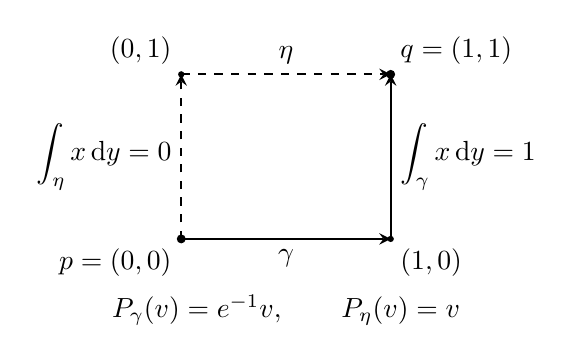
\begin{tikzpicture}[>=stealth,scale=0.95]
		\draw[thick,->] (0,0)--(2.8,0) node[midway,below] {\(\gamma\)};
		\draw[thick,->] (2.8,0)--(2.8,2.2);
		\draw[dashed,thick,->] (0,0)--(0,2.2);
		\draw[dashed,thick,->] (0,2.2)--(2.8,2.2) node[midway,above] {\(\eta\)};
		\fill (0,0) circle (1.7pt) node[below left] {\(p=(0,0)\)};
		\fill (2.8,2.2) circle (1.7pt) node[above right] {\(q=(1,1)\)};
		\fill (2.8,0) circle (1.2pt) node[below right] {\((1,0)\)};
		\fill (0,2.2) circle (1.2pt) node[above left] {\((0,1)\)};
		\node[left] at (0,1.1) {\(\displaystyle\int_\eta x\,\mathrm{d}y=0\)};
		\node[right] at (2.8,1.1) {\(\displaystyle\int_\gamma x\,\mathrm{d}y=1\)};
		\node at (1.4,-0.95) {\(P_\gamma(v)=e^{-1}v,\qquad P_\eta(v)=v\)};
	\end{tikzpicture}
	\caption{同一个联络 \(\alpha=x\,\mathrm{d}y\) 沿两条路径比较相同的两个纤维，得到不同线性同构。实线路径先水平后竖直，虚线路径的顺序相反。}
	\label{g1:fig:path-transport}
\end{figure}

\end{example}

\subsection{由平行移动恢复联络}
\label{g1:subsec:1502:03}

给定局部截面 \(S\)，式 \(S(\gamma(t))-S(\gamma(0))\) 一般没有意义，因为两个向量不在同一纤维。先用反向运输 \(P_{\gamma,0\leftarrow t}\) 把第一个向量送回起点，就能在固定向量空间中取差商。这个操作说明平行移动保存了联络的全部一阶信息。

\begin{theorem}[由运输恢复联络]\label{g1:thm:connection-from-transport}
	设 \(E\to M\) 为实有限秩光滑向量丛，\(M\) 可带边界，\(\nabla\) 为给定联络，\(P\) 是由该联络构造的平行移动。对光滑曲线 \(\gamma:I\to M\)、任意沿曲线的光滑截面 \(s\) 与固定 \(t_0\in I\)，在固定纤维 \(E_{\gamma(t_0)}\) 中有
	\begin{equation}\label{g1:eq:transported-section-derivative}
		\frac{\mathrm{d}}{\mathrm{d}t}\bigl(P_{\gamma,t_0\leftarrow t}s(t)\bigr)
		=P_{\gamma,t_0\leftarrow t}\mathrm{D}_t s.
	\end{equation}
	特别地，若 \(\gamma(0)=p\)、\(\gamma'(0)=v\)，\(S\) 是 \(p\) 附近的光滑截面，则
	\begin{equation}\label{g1:eq:connection-recovery-limit}
		(\nabla_vS)_p
		=\lim_{t\to0}\frac{P_{\gamma,0\leftarrow t}S(\gamma(t))-S(p)}{t}.
	\end{equation}
	若曲线只在零点的一侧有定义，则使用相应的单侧极限。因此同一向量丛上，若两个光滑联络沿所有分片光滑路径产生相同的平行移动，则两个联络相同。
\end{theorem}
\begin{proof}
	先在包含所考察时刻的一个标架域内计算。设从该局部初始时刻到 \(t\) 的平行移动矩阵为 \(U(t)\)，则 \(U'=-BU\)，且 \(U\) 可逆。对 \(U^{-1}U=I\) 求导，得到
	\[
		(U^{-1})'=-U^{-1}U'U^{-1}=U^{-1}B.
	\]
	若 \(s(t)=e(\gamma(t))u(t)\)，则把它运回局部初始纤维后的分量为 \(U(t)^{-1}u(t)\)，而
	\[
		\frac{\mathrm{d}}{\mathrm{d}t}(U^{-1}u)=U^{-1}(u'+Bu).
	\]
	右端恰是 \(\mathrm{D}_ts\) 反向运输后的分量。若固定的 \(t_0\) 不在这一标架域内，先运回局部初始时刻，再接上从该时刻到 \(t_0\) 的固定线性映射；固定线性映射与求导相容，故\eqref{g1:eq:transported-section-derivative}仍成立。

	现在取 \(s=S\circ\gamma\)、\(t_0=0\)，在零点求导。由 \(P_{\gamma,0\leftarrow0}=\operatorname{id}\) 及沿曲线导数与 \(\nabla_{\gamma'}S\) 的相容关系，得到\eqref{g1:eq:connection-recovery-limit}。同一局部计算也证明单侧极限的版本。

	在内部点，每个 \(v\in \mathrm{T}_pM\) 都能由坐标直线给出一条双侧小曲线的初速度，故相同的运输决定所有 \(\nabla_vS\)。在边界点取 \(x^n\ge0\)、\(x(p)=0\) 的图。若 \(v^n\ge0\)，坐标曲线 \(t\mapsto tv\)、\(t\ge0\)，留在半空间中，单侧公式决定 \(\nabla_vS\)。若 \(v^n<0\)，则 \(-v\) 是向内方向，用已经得到的值及 \(\nabla_vS=-\nabla_{-v}S\) 决定它。故两个给定联络若有相同运输，在边界点也相同。零维底流形没有非零切向方向，唯一性同样成立。
\end{proof}

边界处需要保留上述区别。一条以边界点为内部参数时刻、始终留在半空间中的双侧曲线，其法向坐标在该时刻取得局部最小值，所以法向速度必为零。不能用这种曲线代表所有切向量；向内方向由单侧曲线实现，向外方向再通过联络关于方向的线性性决定。

\ProseParagraphBreak

定理恢复的是一个已经给定的联络所产生的运输。若只向每条路径任意指定一个线性同构，即使其中部分映射满足拼接规律，也还不能直接把差商宣布为联络：差商的存在、对路径一阶信息的依赖及所需光滑性都要另外验证。本节得到的是联络与其运输之间的确定关系和唯一性。

\subsection{度量联络和长度保持}
\label{g1:subsec:1502:04}

丛度量 \(g\) 为每个纤维提供内积，存在性已由\cref{g1:thm:bundle-metric-existence}证明。但任意联络不一定在运输时保长；前面 \(x\,\mathrm{d}y\) 的例子，在标准纤维内积下就可能缩短向量。要求“沿途不变的向量保持内积”，应当对应一条关于 \(g\) 与 \(\nabla\) 的微分条件。

\begin{definition}[度量联络]\label{g1:def:metric-connection}
	设 \(E\to M\) 为实有限秩光滑向量丛，\(g\) 是光滑正定丛度量。若联络 \(\nabla\) 对所有局部向量场 \(X\) 和局部截面 \(S,T\) 满足
	\[
		X\bigl(g(S,T)\bigr)=g(\nabla_XS,T)+g(S,\nabla_XT),
	\]
	则称其为关于 \(g\) 的\term[dulianglianluo]{度量联络}[metric connection]，也称与 \(g\) 相容。这就是诱导张量联络下的 \(\nabla g=0\)。
\end{definition}

\begin{proposition}[度量相容与平行移动]\label{g1:prop:metric-parallel-transport}
	设 \(M\) 为有限维光滑流形，允许有边界，\(E\to M\) 为实有限秩光滑向量丛，带光滑正定度量 \(g\) 和联络 \(\nabla\)。以下条件等价：
	\begin{enumerate}
		\item \(\nabla g=0\)。
		\item 在每个局部标架 \(e\) 中，令 \(G=(g(e_i,e_j))\)、\(\nabla e=eA\)，则
		\begin{equation}\label{g1:eq:metric-connection-matrix}
			\mathrm{d}G=A^{\mathsf T}G+GA.
		\end{equation}
		\item 对每条光滑曲线及任意两个沿曲线的光滑截面 \(s,t\)，有
		\[
			\frac{\mathrm{d}}{\mathrm{d}\tau}g(s(\tau),t(\tau))
			=g(\mathrm{D}_\tau s,t)+g(s,\mathrm{D}_\tau t).
		\]
		\item 每条有限分片光滑路径的平行移动都是端点纤维之间的内积等距同构。
	\end{enumerate}
	因而也可以把最后一项等价地写为所有平行移动保持每个向量的长度。
\end{proposition}
\begin{proof}
	将度量相容条件应用于局部基截面 \(e_i,e_j\)。\(\nabla e_j=\sum_k e_kA^k{}_j\)，所以右边的两个矩阵分别为 \(A^{\mathsf T}G\) 和 \(GA\)，得到第二项。反过来，把任意截面写成 \(eu,ev\)，对 \(u^{\mathsf T}Gv\) 使用乘积法则，第二项就给出第一项。

	沿曲线记 \(B=A(\gamma')\)。第二项拉回曲线成为 \(G'=B^{\mathsf T}G+GB\)。于是
	\[
		\frac{\mathrm{d}}{\mathrm{d}\tau}(u^{\mathsf T}Gv)
		=(u'+Bu)^{\mathsf T}Gv+u^{\mathsf T}G(v'+Bv),
	\]
	恰为第三项。两个截面都平行时，右端为零，故内积沿每个光滑片恒定；连续性使这些常值在分段端点吻合。这证明第四项。

	反过来假设第四项。对 \(p\) 附近的局部截面 \(S,T\) 及过 \(p\) 的曲线，令
	\[
		\widehat S(\tau)=P_{\gamma,0\leftarrow\tau}S(\gamma(\tau)),\qquad
		\widehat T(\tau)=P_{\gamma,0\leftarrow\tau}T(\gamma(\tau)).
	\]
	运输保内积，故 \(g_{\gamma(\tau)}(S,T)=g_p(\widehat S(\tau),\widehat T(\tau))\)。在零点求导，再用\cref{g1:thm:connection-from-transport}，得到方向 \(v=\gamma'(0)\) 上的度量相容等式。内部点可取任意 \(v\)；边界处先取向内的单侧曲线，再利用等式两边关于 \(v\) 的线性性处理向外方向。因此第一项成立。

	最后，保内积必然保长度；反过来，实内积由
	\[
		g(v,w)=\frac12\bigl(|v+w|_g^2-|v|_g^2-|w|_g^2\bigr)
	\]
	恢复。平行移动已经线性，故保全部向量的长度也保证保内积。
\end{proof}

在正交归一标架中 \(G=I_r\)，矩阵条件简化为 \(A^{\mathsf T}+A=0\)，即每个 \(A(X)\) 为斜对称矩阵。在一般标架中却不能直接要求 \(A\) 斜对称，必须保留 \(\mathrm{d}G\) 这一项。度量可能随基点变化，而非正交标架自身的长度也会变化。

\begin{proposition}[度量联络的存在]\label{g1:prop:metric-connection-existence}
	设 \(M\) 为有限维、Hausdorff、第二可数的光滑流形，允许有边界，\(E\to M\) 为实有限秩光滑向量丛，\(g\) 为光滑正定丛度量。则 \(E\) 上存在与 \(g\) 相容的联络。给定一个度量联络后，所有其他度量联络恰为 \(\nabla+K\)，其中 \(K\in\Omega^1(M;\operatorname{End}E)\) 满足每个 \(K(X)\) 关于 \(g\) 斜伴随。
\end{proposition}
\begin{proof}
	由\cref{g1:thm:connection-existence}取任意联络 \(\nabla^0\)，再修正它不保持度量的部分。定义
	\[
		Q_X(S,T)=Xg(S,T)-g(\nabla^0_XS,T)-g(S,\nabla^0_XT).
	\]
	Leibniz 法则使这里对 \(S,T\) 的导数项在乘以函数时抵消，故 \(Q\) 对 \(X,S,T\) 都是逐点线性的；它还是光滑的，且对 \(S,T\) 对称。正定性使每个纤维的 \(g\) 非退化，因此存在唯一的 \(C_X\in\operatorname{End}(E)\)，满足
	\[
		g(C_XS,T)=\frac12Q_X(S,T).
	\]
	在局部标架中，若 \(Q_X\) 的对称矩阵为 \(Q(X)\)，这个算子为 \(C_X=\tfrac12G^{-1}Q(X)\)。矩阵逆光滑，故 \(C\) 是光滑的 \(\operatorname{End}E\) 值一形式。

	由\cref{g1:prop:connection-affine-space}，\(\nabla=\nabla^0+C\) 仍是联络。对称性给出
	\begin{align*}
		(\nabla_Xg)(S,T)&=Q_X(S,T)-g(C_XS,T)-g(S,C_XT)\\
		&=Q_X(S,T)-\tfrac12Q_X(S,T)-\tfrac12Q_X(S,T)=0.
	\end{align*}
	因此修正后的联络与度量相容。在矩阵语言中，这一修正是
	\[
		A=A^0+\frac12G^{-1}\bigl(\mathrm{d}G-(A^0)^{\mathsf T}G-GA^0\bigr).
	\]

	若 \(\widetilde\nabla=\nabla+K\)，其中 \(\nabla\) 已度量相容，则
	\[
		(\widetilde\nabla_Xg)(S,T)=-g(K(X)S,T)-g(S,K(X)T).
	\]
	因而 \(\widetilde\nabla\) 也相容，当且仅当每个 \(K(X)\) 斜伴随。这证明了最后的全部刻画。
\end{proof}

\begin{example}\label{g1:exm:rotating-metric-transport}
	在平凡二维丛中取标准内积，令
	\[
		J=\begin{pmatrix}0&-1\\1&0\end{pmatrix},\qquad A=J\,\alpha
	\]
	其中 \(\alpha\) 是任意实一形式。因为 \(J^{\mathsf T}=-J\)，这是度量联络。沿路径记 \(\theta(t)=\int_{t_0}^t \alpha(\gamma'(v))\,\mathrm{d}v\)，则
	\[
		u(t)=\exp(-\theta(t)J)u_0
		=\begin{pmatrix}\cos\theta(t)&\sin\theta(t)\\-\sin\theta(t)&\cos\theta(t)\end{pmatrix}u_0.
	\]
	矩阵求导给出 \(u'=-J\,\alpha(\gamma')u\)，因此这就是平行解。它保持长度，转角却是 \(-\theta\)，再次显示平行方程中的负号。保长不表示每条环路运输都为恒等；它只把可能的运输限制在纤维的正交变换之中。
\end{example}

% 纲要条目排为编号小节标题，并进入目录与书签；说明段仍保留于纲要注释中。

% !TeX root = ../../Book1.tex
% 纲要标题：### 15.3 曲率与结构方程
% 纲要位置：几何学计划纲要.md，第 708 行。
% 正文状态：初稿；尚未正式审核。

% 纲要内容开始
% 
% * 二阶协变微分及张量性
% * 外协变微分与曲率矩阵
% * 曲率的换标架规律与小环路运输
% * Bianchi 恒等式的结构证明
% 
% 纲要内容结束

\section{曲率与结构方程}
\label{g1:sec:1503}

联络使我们能够沿路径比较纤维中的向量，但两条同起点、同终点的路径未必给出同一种比较。在第九章的曲面例子中，绕小圈后的转角由曲率控制。一般向量丛中的返回变换可以伸缩、剪切，也可以旋转，因而需要一个取值于纤维自同态的对象来记录这种变化。本节把它从二阶协变微分中构造出来，再说明它怎样出现在小环路的运输中。

\ProseParagraphBreak

以下 \(E\to M\) 是有限秩实光滑向量丛，\(M\) 有限维、Hausdorff、第二可数，允许边界，\(\nabla\) 是光滑联络。沿用行标架 \(e\)、列分量 \(u\) 和 \(\nabla s=e(\mathrm{d}u+Au)\) 的约定。外微分及分次乘积法则使用\cref{g1:thm:exterior-derivative}；向量场括号的顺序仍为 \([X,Y]=XY-YX\)。边界处使用局部光滑延拓定义括号；\eqref{g1:eq:lie-bracket-product}中的乘法法则由同一坐标计算继续成立。

\subsection{二阶协变微分及张量性}
\label{g1:subsec:1503:01}

单独的 \(\nabla_X\nabla_Ys\) 会依赖 \(Y\) 及 \(s\) 在邻近点的变化。交换 \(X,Y\) 可以消去一部分二阶项，但若方向场自身不交换，还须减去它们的 Lie 括号所贡献的一阶变化。这正是第八章曲面曲率定义中出现第三项的原因，现在同一构造适用于任意向量丛。

\begin{definition}[丛联络的曲率]\label{g1:def:bundle-curvature}
	设 \(E\to M\) 为实光滑向量丛，\(\nabla\) 为其联络，允许 \(M\) 带边界。定义
	\[
		R^\nabla(X,Y)s=\nabla_X\nabla_Ys-\nabla_Y\nabla_Xs-\nabla_{[X,Y]}s,
		\qquad X,Y\in\mathfrak X(M),\quad s\in\Gamma(E).
	\]
	称 \(R^\nabla\) 为该联络的曲率；不致混淆时记作 \(R\)。
\end{definition}

\begin{proposition}[曲率的张量性]\label{g1:prop:bundle-curvature-tensorial}
	设 \(E\to M\) 为实光滑向量丛，\(M\) 可带边界，\(\nabla\) 为光滑联络。对光滑向量场 \(X,Y\) 和光滑截面 \(s\)，令
	\[
		R(X,Y)s=\nabla_X\nabla_Ys-\nabla_Y\nabla_Xs-\nabla_{[X,Y]}s.
	\]
	此运算对 \(X,Y,s\) 均为 \(C^\infty(M)\) 线性，并对前两个变量反对称。因此它唯一确定一个光滑截面
	\[
		R\in\Omega^2(M;\operatorname{End}E)
		=\Gamma(\Lambda^2\mathrm{T}^*M\otimes\operatorname{End}E).
	\]
	在点 \(p\)，\(R_p(v,w)\) 是 \(E_p\) 上的线性自同态，只依赖 \(v,w\in \mathrm{T}_pM\) 和被作用的纤维向量。
\end{proposition}
\begin{proof}
	实多线性和反对称性由定义得到。对光滑函数 \(f\)，先回忆\eqref{g1:eq:lie-bracket-product}的 \([fX,Y]=f[X,Y]-Y(f)X\)。该等式在边界处仍由局部延拓成立。于是
	\begin{align*}
		R(fX,Y)s
		&=f\nabla_X\nabla_Ys-\nabla_Y(f\nabla_Xs)-\nabla_{f[X,Y]-Y(f)X}s\\
		&=fR(X,Y)s.
	\end{align*}
	两个含 \(Y(f)\nabla_Xs\) 的项相消；第二变量的函数线性再由反对称性得到。

	对截面 \(fs\)，展开
	\[
		\nabla_X\nabla_Y(fs)
		=X(Yf)s+(Yf)\nabla_Xs+(Xf)\nabla_Ys+f\nabla_X\nabla_Ys.
	\]
	交换 \(X,Y\) 后，一阶交叉项抵消。再减去 \(\nabla_{[X,Y]}(fs)\)，额外剩余项为 \((X(Yf)-Y(Xf)-[X,Y]f)s=0\)，故 \(R(X,Y)(fs)=fR(X,Y)s\)。在局部坐标标架和丛标架中展开三个输入，函数线性把所有分量移到外面，点处结果便只依赖这些分量在该点的值。各基向量上的结果光滑，故得到所述光滑丛值二形式。
\end{proof}

这里的“二形式”只计算两个切向输入；它的输出不是实数，而是一个还可以作用于纤维向量的线性映射。若 \(E=\mathrm{T}M\)，这就是\cref{g1:def:surface-curvature-tensor}所用曲率的高维版本；若 \(E\) 是一条线丛，则每个纤维自同态只是一个实数倍。

\begin{definition}\label{g1:def:flat-connection}
	若光滑向量丛联络的曲率处处为零，即 \(R^\nabla=0\)，称该联络为\term[pingtanlianluo]{平坦联络}[flat connection]。这个条件针对给定联络；说一个丛具有平坦联络，还须指定或证明这样的联络存在。
\end{definition}

平坦的定义目前只表达一个局部微分条件。它是否足以得到平行标架，以及是否使所有同端点路径的运输相同，需要\secref{g1:sec:1505}的构造来回答。

\subsection{外协变微分与曲率矩阵}
\label{g1:subsec:1503:02}

普通外微分作用于实值形式，联络作用于丛截面。要把它们组织成同一个运算，回顾\cref{g1:def:bundle-valued-form}的记号
\[
	\Omega^k(M;E)=\Gamma(\Lambda^k\mathrm{T}^*M\otimes E).
\]
其元素在一点接受 \(k\) 个切向量，交替多线性地输出一个纤维向量。在标架 \(e\) 中写为 \(\eta=\sum_a\eta^a\otimes e_a\)，其中 \(\eta^a\) 是普通 \(k\) 形式；简记成 \(e\eta_e\)，\(\eta_e=(\eta^a)\) 为列。换标架 \(e'=eg\) 时，列分量变为 \(\eta_{e'}=g^{-1}\eta_e\)。

\ProseParagraphBreak

矩阵值形式相乘时，同时作矩阵乘法和形式楔积。若 \(B\) 是矩阵值 \(p\) 形式、\(C\) 是矩阵值 \(q\) 形式，规定
\[
	(B\wedge C)^a{}_b=\sum_c B^a{}_c\wedge C^c{}_b.
\]
它结合，但一般不满足普通标量形式的分次交换律。特别地，\(A\wedge A\) 未必为零，因为不同矩阵系数未必交换。矩阵乘列形式也按同样规则定义。

\begin{proposition}[外协变微分]\label{g1:prop:exterior-covariant-derivative}
	设 \(\nabla\) 为实光滑向量丛 \(E\to M\) 上的联络。存在唯一的实线性局部算子
	\[
		\mathrm{d}_\nabla:\Omega^k(M;E)\longrightarrow\Omega^{k+1}(M;E)
	\]
	在零次截面上等于 \(\nabla\)，并满足对标量 \(p\) 形式 \(\alpha\) 与丛值形式 \(\eta\)，
	\[
		\mathrm{d}_\nabla(\alpha\wedge\eta)
		=\mathrm{d}\alpha\wedge\eta+(-1)^p\alpha\wedge\mathrm{d}_\nabla\eta.
	\]
	在联络矩阵为 \(A\) 的标架中，它由
	\begin{equation}\label{g1:eq:exterior-covariant-local}
		\mathrm{d}_\nabla(e\eta_e)=e(\mathrm{d}\eta_e+A\wedge\eta_e)
	\end{equation}
	给出，称为\term[waixiebianweifen]{外协变微分}[exterior covariant derivative]。
\end{proposition}
\begin{proof}
	先按局部公式定义。令 \(e'=eg\)，则\eqref{g1:eq:connection-frame-change}给出 \(A'=g^{-1}Ag+g^{-1}\mathrm{d}g\)，而微分 \(g^{-1}g=I\) 得
	\[
		\mathrm{d}(g^{-1})=-g^{-1}(\mathrm{d}g)g^{-1}.
	\]
	于是
	\begin{align*}
		\mathrm{d}(g^{-1}\eta_e)+A'\wedge(g^{-1}\eta_e)
		&=-g^{-1}(\mathrm{d}g)g^{-1}\wedge\eta_e+g^{-1}\mathrm{d}\eta_e\\
		&\quad+g^{-1}A\wedge\eta_e+g^{-1}(\mathrm{d}g)g^{-1}\wedge\eta_e\\
		&=g^{-1}(\mathrm{d}\eta_e+A\wedge\eta_e).
	\end{align*}
	结果按丛值形式的分量变换，因而粘成整体算子。它在零次时就是联络，分次乘积法则则由普通外微分的规则及 \(A\wedge\alpha=(-1)^p\alpha\wedge A\) 得到；这里 \(\alpha\) 是标量，允许这样换序。

	反过来，任意局部丛值形式都是 \(\sum_a\eta^a\otimes e_a\)。对每项使用规定的乘积法则，结果只能为 \(\mathrm{d}\eta^a\otimes e_a+(-1)^k\eta^a\wedge\nabla e_a\)，移过一次形式后正是\eqref{g1:eq:exterior-covariant-local}，所以唯一。
\end{proof}

后文有时将 \(\mathrm{d}_\nabla\) 简记为 \(\mathrm{D}\)，将自同态丛诱导联络的外协变微分简记为 \(\mathrm{D}_{\operatorname{End}}\)。普通外微分平方为零，外协变微分却不一定如此。差别正好是曲率。

\begin{theorem}[曲率的结构方程]\label{g1:thm:curvature-structure-equation}
	设 \(\nabla\) 为实光滑向量丛 \(E\to M\) 上的联络，\(A\) 是某局部标架中的联络矩阵。曲率 \(R\) 在该标架中的矩阵值二形式为
	\begin{equation}\label{g1:eq:curvature-matrix}
		F=\mathrm{d}A+A\wedge A.
	\end{equation}
	对每个 \(\eta\in\Omega^k(M;E)\)，有 \(\mathrm{d}_\nabla^2\eta=R\wedge\eta\)，局部分量即 \(F\wedge\eta_e\)。
\end{theorem}
\begin{proof}
	由局部公式及 \(\mathrm{d}^2=0\)，逐项计算
	\begin{align*}
		(\mathrm{d}+A\wedge)^2\eta_e
		&=\mathrm{d}A\wedge\eta_e-A\wedge\mathrm{d}\eta_e
		+A\wedge\mathrm{d}\eta_e+A\wedge A\wedge\eta_e\\
		&=(\mathrm{d}A+A\wedge A)\wedge\eta_e.
	\end{align*}
	还须确认这确实是先前定义的曲率。对零次截面 \(s=e u\)，把两次协变导数展开并扣除括号项，导数作用于 \(u\) 的项抵消，余下
	\[
		e^{-1}R(X,Y)s
		=\bigl(X(A(Y))-Y(A(X))-A([X,Y])
		+A(X)A(Y)-A(Y)A(X)\bigr)u.
	\]
	由\eqref{g1:eq:exterior-one-form-evaluation}，前三项是 \(\mathrm{d}A(X,Y)\)，后两项是 \((A\wedge A)(X,Y)\)，故所列 \(F\) 表示 \(R\)。一般次数的结论随第一段计算得到。
\end{proof}

在坐标 \(x^i\) 中写 \(A=\sum_i A_i\,\mathrm{d}x^i\)，则
\[
	F=\sum_{i<j}F_{ij}\,\mathrm{d}x^i\wedge\mathrm{d}x^j,
	\qquad F_{ij}=\partial_iA_j-\partial_jA_i+[A_i,A_j].
\]
这里对 \(i<j\) 求和，没有额外的 \(1/2\)。最后一项是矩阵交换子，它记录纤维方向的两次线性变化不交换，不能用标量一形式自楔为零的规则删掉。

\begin{example}[常系数也可能有曲率]\label{g1:exm:constant-noncommuting-connection}
	在 \(\mathbb R^2\times\mathbb R^2\) 的标准标架中取
	\[
		A=B\,\mathrm{d}x+C\,\mathrm{d}y,\qquad
		B=\begin{pmatrix}0&1\\0&0\end{pmatrix},\quad
		C=\begin{pmatrix}0&0\\1&0\end{pmatrix}.
	\]
	虽然 \(\mathrm{d}A=0\)，但
	\[
		F=[B,C]\,\mathrm{d}x\wedge\mathrm{d}y
		=\begin{pmatrix}1&0\\0&-1\end{pmatrix}\mathrm{d}x\wedge\mathrm{d}y\ne0.
	\]
	因此系数恒定、底空间单连通，都不能替代曲率为零。沿一条路径的方程只涉及一个时间变量；同时要求两个方向上的运输相容，才会发现这里的交换子。
\end{example}

在线丛的局部标架中，\(A\) 是标量一形式，\(A\wedge A=0\)，所以 \(F=\mathrm{d}A\)。在第九章的正向正交曲面标架中，\eqref{g1:eq:surface-frame-connection}给出
\[
	A=\begin{pmatrix}0&-\omega\\\omega&0\end{pmatrix},\qquad
	F=\begin{pmatrix}0&-\mathrm{d}\omega\\\mathrm{d}\omega&0\end{pmatrix}.
\]
该例中 \(A\wedge A=0\)，并由\eqref{g1:eq:surface-curvature-form}得到 \(\mathrm{d}\omega=-K\,\mathrm{d}A\)。这里最后的 \(\mathrm{d}A\) 沿用曲面面积形式的记号，与前面“对矩阵 \(A\) 求外微分”的 \(\mathrm{d}A\) 对象不同；在一般丛公式中，\(A\) 始终表示联络矩阵。

\subsection{曲率的换标架规律与小环路运输}
\label{g1:subsec:1503:03}

联络矩阵的变换律含有 \(\mathrm{d}g\)，说明它不按张量变换。曲率已经证明是张量，因而应当只发生纤维基变换，不再出现新的导数项。

\begin{proposition}[曲率的换标架公式]\label{g1:prop:curvature-frame-change}
	若同一实向量丛联络在标架 \(e\) 与 \(e'=eg\) 中的曲率矩阵分别为 \(F,F'\)，则
	\[
		F'=g^{-1}Fg.
	\]
	因此曲率是否为零与标架无关；对固定的切向输入，所得自同态的迹、行列式等共轭不变量也与标架无关。
\end{proposition}
\begin{proof}
	对任意列向量 \(u'\)，同一截面为 \(s=e'u'=e(gu')\)。曲率的纤维线性给出 \(R(X,Y)s=eF(X,Y)g u'\)，另一方面它等于 \(e'F'(X,Y)u'=egF'(X,Y)u'\)。因此 \(Fg=gF'\)，得到结论。这个证明也说明变换律中没有导数项的原因：\(R\) 对截面是逐点线性的。
\end{proof}

\begin{proposition}[小方环的运输]\label{g1:prop:small-loop-curvature}
	设 \(p\) 是光滑流形 \(M\) 的内点，\(\dim M\geq2\)，\(E\to M\) 为秩 \(r\) 实光滑向量丛，\(\nabla\) 为其光滑联络。取以 \(p\) 为原点的坐标及丛标架，记联络矩阵为 \(A\)，曲率矩阵为 \(F=\mathrm{d}A+A\wedge A=\sum_{i<j}F_{ij}\,\mathrm{d}x^i\wedge\mathrm{d}x^j\)。令 \(\gamma_\varepsilon\) 依次沿坐标方形的 \(+x^1,+x^2,-x^1,-x^2\) 四边行进，每边坐标长度为 \(\varepsilon>0\)，其余坐标为零。则在 \(E_p\) 的该标架中，
	\begin{equation}\label{g1:eq:small-loop-curvature}
		P_{\gamma_\varepsilon}
		=I-\varepsilon^2F_{12}(p)+O(\varepsilon^3).
	\end{equation}
	余项指选定矩阵范数下存在与充分小 \(\varepsilon\) 无关的常数 \(C\)，使其范数不超过 \(C\varepsilon^3\)。
\end{proposition}
\begin{proof}
	先用换标架消去一点处的联络系数。令 \(g(x)=I-\sum_i x^iA_i(p)\)，缩小邻域可使 \(g\) 可逆。由变换律，\(g(p)=I\) 且 \(A'_i(p)=A_i(p)+\partial_i g(p)=0\)。新旧标架在基点相同，故返回映射的基点矩阵不变，曲率矩阵在基点也不变。以下在这组新标架中计算并省去撇号。

	四边上 \(A_i=O(\varepsilon)\)。把一条边用坐标长度参数化，平行移动的矩阵满足 \(U'=-B(t)U\)、\(U(0)=I\)，其中时间长度为 \(\varepsilon\)、\(\|B\|\leq C\varepsilon\)。积分方程及\cref{g1:lem:gronwall-estimate}给出 \(\|U\|\leq e^{C\varepsilon^2}\) 和 \(U-I=O(\varepsilon^2)\)，于是再次代回积分方程得
	\[
		U=I-\int_{\text{该边}}A+O(\varepsilon^4).
	\]
	把四段按实际行进顺序相乘，两个积分项的乘积也是 \(O(\varepsilon^4)\)，所以
	\[
		P_{\gamma_\varepsilon}=I-\oint_{\gamma_\varepsilon}A+O(\varepsilon^4).
	\]
	对每个矩阵条目用\cref{g1:thm:stokes-corners}的矩形情形，按\eqref{g1:eq:rectangle-boundary-signs}取正向边界，再对系数作 Taylor 展开，有
	\[
		\oint_{\gamma_\varepsilon}A
		=\int_0^\varepsilon\int_0^\varepsilon
		(\partial_1A_2-\partial_2A_1)(s,t,0,\ldots,0)\,\mathrm{d}s\,\mathrm{d}t
		=\varepsilon^2F_{12}(p)+O(\varepsilon^3).
	\]
	最后一步使用光滑性和 \(A(p)=0\)，此时基点的交换子项为零。结合两式得到结论。矩形缩在内点坐标域内，故没有额外的边界条件。
\end{proof}

% !TeX root = ../Book1.tex
% 两条同端点路径及其组成的小正向回路。
\begin{figure}[htbp]
	\centering
	\begin{tikzpicture}[font=\small,scale=1.1]
		\fill[GeometryBlueLight] (0,0) rectangle (3,2.1);
		\draw[->,GeometryGray] (-0.4,0)--(3.8,0) node[right] {\(x^1\)};
		\draw[->,GeometryGray] (0,-0.4)--(0,2.8) node[above] {\(x^2\)};
		\draw[GeometryBlue,very thick,->] (0,0)--(1.7,0);
		\draw[GeometryBlue,very thick] (1.7,0)--(3,0);
		\draw[GeometryBlue,very thick,->] (3,0)--(3,1.3);
		\draw[GeometryBlue,very thick] (3,1.3)--(3,2.1);
		\draw[orange!80!black,very thick,->] (0,0)--(0,1.3);
		\draw[orange!80!black,very thick] (0,1.3)--(0,2.1);
		\draw[orange!80!black,very thick,->] (0,2.1)--(1.7,2.1);
		\draw[orange!80!black,very thick] (1.7,2.1)--(3,2.1);
		\fill (0,0) circle[radius=1.8pt] node[below left] {\(p\)};
		\fill (3,2.1) circle[radius=1.8pt] node[above right] {\(q\)};
		\node[below] at (3,0) {\(\varepsilon\)};
		\node[left] at (0,2.1) {\(\varepsilon\)};
		\node[GeometryBlue] at (2.3,0.35) {\(\alpha\)};
		\node[orange!80!black] at (0.65,1.7) {\(\beta\)};
		\node[align=center] at (1.6,1.0) {先沿 \(\alpha\)，再沿 \(\beta^{-1}\)\\\(P_{\beta}^{-1}P_{\alpha}\)};
	\end{tikzpicture}
	\caption{两条路径都从 \(p\) 到 \(q\)。用 \(\beta\) 的逆向运输把 \(\alpha\) 的结果带回 \(E_p\)，得到正向小回路的返回变换。它与恒等变换之差的面积首项为 \(-\varepsilon^2F_{12}(p)\)；两边长度在图中仅作示意。}
	\label{g1:fig:curvature-loop}
\end{figure}


\cref{g1:fig:curvature-loop}中的两条折线路径有相同端点，但沿第一条出发、沿第二条反向返回，会形成这个方环。\eqref{g1:eq:small-loop-curvature}说明它们的差首先在面积阶出现，系数就是曲率。负号来自平行方程 \(u'=-A(\dot\gamma)u\) 和所选绕行方向；换成反向环路便反号。一般矩阵系数不交换，不能把小环路的一阶面积近似误写成任意大环路上的 \(P_\gamma=\exp(-\int F)\)。

\subsection{Bianchi 恒等式的结构证明}
\label{g1:subsec:1503:04}

曲率是联络的二阶变化，它自身并不是任意的矩阵值二形式：结构方程强制它满足一个协变微分恒等式。为了准确写出这个式子，先将\cref{g1:prop:induced-connections}给出的 \(\operatorname{End}E\) 联络延拓到自同态值形式。对矩阵值 \(k\) 形式 \(B\)，其外协变微分为
\begin{equation}\label{g1:eq:endomorphism-exterior-derivative}
	\mathrm{d}_{\nabla^{\operatorname{End}}}B
	=\mathrm{d}B+A\wedge B-(-1)^k B\wedge A.
\end{equation}
这里把整体自同态值形式与其局部矩阵暂用同一字母。对 \(B=\beta C\)，其中 \(\beta\) 为标量 \(k\) 形式、\(C\) 为自同态矩阵函数，先用 \(\nabla^{\operatorname{End}}C=\mathrm{d}C+AC-CA\)，再用外协变微分的分次乘积法则，就得到该式；一般 \(B\) 是这类项之和。因而它来自已定义的诱导联络，而不是任意补入的修正项。

下面的\term[bianchihengdengshi]{Bianchi 恒等式}[Bianchi identity]\footnote{Bianchi，Luigi Bianchi（1856--1928），意大利数学家，研究曲面、Riemann 几何及连续变换群。}表达曲率的这种相容性。

\begin{theorem}[Bianchi 恒等式]\label{g1:thm:bianchi-identity}
	设 \(E\to M\) 为实光滑向量丛，\(\nabla\) 为光滑联络，\(R\) 为其曲率，\(\nabla^{\operatorname{End}}\) 为在 \(\operatorname{End}E\) 上诱导的联络。在任一光滑局部标架中，记 \(A,F\) 分别为联络及曲率的矩阵形式。则
	\[
		\mathrm{d}_{\nabla^{\operatorname{End}}}R=0.
	\]
	局部矩阵形式为
	\begin{equation}\label{g1:eq:bianchi-matrix}
		\mathrm{d}F+A\wedge F-F\wedge A=0.
	\end{equation}
\end{theorem}
\begin{proof}
	代入结构方程 \(F=\mathrm{d}A+A\wedge A\)。由于 \(A\) 是一次形式，
	\[
		\mathrm{d}F=\mathrm{d}A\wedge A-A\wedge\mathrm{d}A.
	\]
	另外
	\[
		A\wedge F-F\wedge A
		=A\wedge\mathrm{d}A+A\wedge A\wedge A
		-\mathrm{d}A\wedge A-A\wedge A\wedge A.
	\]
	两式相加，各项成对抵消。上述局部表达是整体 \(\operatorname{End}E\) 联络的外协变微分，所以每张图中为零就意味着整体为零。整个论证只用外微分平方为零、分次乘积法则及矩阵乘法结合性，不要求度量或无挠条件。
\end{proof}

这个恒等式通常称为第二 Bianchi 恒等式；切丛上另有涉及挠率的第一 Bianchi 恒等式，将在下一节得到。

\ProseParagraphBreak

在坐标向量场上，它的可计算形式是
\[
	\partial_iF_{jk}+\partial_jF_{ki}+\partial_kF_{ij}
	+[A_i,F_{jk}]+[A_j,F_{ki}]+[A_k,F_{ij}]=0.
\]
因此一般不能删掉交换子而断言 \(\mathrm{d}F=0\)。在线丛上矩阵系数交换，式子才退化为普通的 \(\mathrm{d}F=0\)。在二维底流形上，恒等式因三形式为零而自动成立；它既不迫使二维曲率为零，也不说明联络可以取成零矩阵。

% 纲要条目排为编号小节标题，并进入目录与书签；说明段仍保留于纲要注释中。

% !TeX root = ../../Book1.tex
% 纲要标题：### 15.4 切丛联络与挠率
% 纲要位置：几何学计划纲要.md，第 715 行。
% 正文状态：初稿；尚未正式审核。

% 纲要内容开始
% 
% * 挠率的坐标无关定义
% * 无挠性和坐标标架
% * 第一结构方程
% * 切丛与一般向量丛的区别
% 
% 纲要内容结束

\section{切丛联络与挠率}
\label{g1:sec:1504}

一般向量丛的联络接受一个切向量方向和一个丛截面，输出同一丛的截面。对切丛，方向场和被微分的截面恰好都是向量场，因而可以交换二者，还可以把结果与 Lie 括号比较。这种额外的比较产生挠率。曲率考察同一向量连续经过两次协变微分后的差别；挠率则从一次协变微分出发，比较方向与被微分向量的交换。

\ProseParagraphBreak

本节 \(\nabla\) 是 \(\mathrm{T}M\) 上的光滑联络，\(M\) 有限维、Hausdorff、第二可数，允许边界。涉及坐标向量场的局部可实现性时，将明确限制在内点。度量不是挠率定义所需的数据，以下也不默认联络保持任何度量。

\subsection{挠率的坐标无关定义}
\label{g1:subsec:1504:01}

在 Euclid 空间的通常导数下，\(\partial_XY-\partial_YX=[X,Y]\)。因此，直接把 \(\nabla_XY-\nabla_YX\) 当成偏离 Euclid 情形的量并不合适：即使使用通常导数，只要所选方向场不交换，它也可能不为零。应当先减去由方向场本身造成的 Lie 括号。

\begin{definition}[挠率]\label{g1:def:torsion}
	切丛联络 \(\nabla\) 的\term[naolv]{挠率}[torsion]定义为
	\begin{equation}\label{g1:eq:torsion-definition}
		T^\nabla(X,Y)=\nabla_XY-\nabla_YX-[X,Y].
	\end{equation}
	若 \(T^\nabla=0\)，称 \(\nabla\) 为\term[wunaolianluo]{无挠联络}[torsion-free connection]。下文不致混淆时简记为 \(T\)。
\end{definition}

第七章也用“挠率”表示空间曲线的标量 \(\tau\)，它描述 Frenet 标架的转动。这里的 \(T\) 是切丛联络的二输入张量，二者的定义和所需数据不同，不能因中文名称相同便代入同一个公式。

\begin{proposition}[挠率的张量性]\label{g1:prop:torsion-tensorial}
	设 \(M\) 为可带边界的光滑流形，\(\nabla\) 为 \(\mathrm{T}M\) 上的光滑线性联络，\(T\) 为其挠率。则 \(T\) 是一个光滑的切丛值二形式，即 \(T\in\Omega^2(M;\mathrm{T}M)\)。在任意局部标架 \((e_i)\) 中，若
	\[
		\nabla_{e_i}e_j=\sum_k\Gamma^k_{ij}e_k,\qquad
		[e_i,e_j]=\sum_k c^k_{ij}e_k,
	\]
	则
	\begin{equation}\label{g1:eq:torsion-frame-components}
		T(e_i,e_j)=\sum_k\bigl(\Gamma^k_{ij}-\Gamma^k_{ji}-c^k_{ij}\bigr)e_k.
	\end{equation}
\end{proposition}
\begin{proof}
	由定义，\(T\) 实双线性且反对称。用\eqref{g1:eq:lie-bracket-product}中的 \([fX,Y]=f[X,Y]-Y(f)X\)，得到
	\begin{align*}
		T(fX,Y)
		&=f\nabla_XY-\nabla_Y(fX)-[fX,Y]\\
		&=f\nabla_XY-Y(f)X-f\nabla_YX-f[X,Y]+Y(f)X\\
		&=fT(X,Y).
	\end{align*}
	反对称性随后给出第二个输入的函数线性。因此在局部标架中展开 \(X,Y\)，结果只依赖它们在求值点的分量；各分量又光滑，故为光滑张量。把两个输入取成 \(e_i,e_j\)，直接代入定义便得分量公式。边界处同样的局部延拓计算成立。
\end{proof}

在\secref{g1:sec:0803}中，曲面的诱导联络已经满足 \(\nabla_XY-\nabla_YX=[X,Y]\)，见\cref{g1:prop:surface-connection-properties}。现在可以把该性质简洁地表述为“曲面的诱导联络无挠”。这不是所有切丛联络自动具有的性质。

\subsection{无挠性和坐标标架}
\label{g1:subsec:1504:02}

坐标标架满足 \([\partial_i,\partial_j]=0\)，所以\eqref{g1:eq:torsion-frame-components}化为
\[
	T(\partial_i,\partial_j)=\sum_k(\Gamma^k_{ij}-\Gamma^k_{ji})\partial_k.
\]
于是无挠性等价于每个坐标图中 \(\Gamma^k_{ij}=\Gamma^k_{ji}\)。这里两个下指标分别表示微分方向和被微分向量；只有在坐标标架中，才能不加修正地使用这条对称性判据。一般标架中的正确判据是 \(\Gamma^k_{ij}-\Gamma^k_{ji}=c^k_{ij}\)。

\begin{proposition}[无挠联络的存在与差]\label{g1:prop:torsion-free-affine-space}
	设 \(M\) 为有限维、Hausdorff、第二可数的光滑流形，允许有边界。则 \(\mathrm{T}M\) 上存在无挠光滑联络。对任意两个光滑切丛联络 \(\nabla,\nabla'\)，若 \(\nabla' =\nabla+B\)，其中 \(B\in\Omega^1(M;\operatorname{End}(\mathrm{T}M))\)，则
	\begin{equation}\label{g1:eq:torsion-difference}
		T^{\nabla'}(X,Y)=T^\nabla(X,Y)+B(X)Y-B(Y)X.
	\end{equation}
	无挠联络组成一个仿射空间，其平移向量空间为 \(\Gamma(\operatorname{Sym}^2\mathrm{T}^*M\otimes \mathrm{T}M)\)。
\end{proposition}
\begin{proof}
	将 \(\nabla'\) 代入挠率定义，Lie 括号项相消，就得到差公式。由\cref{g1:thm:connection-existence}，先任选一个切丛联络 \(\nabla\)。其挠率已经证明为张量，所以
	\[
		\nabla^0_XY=\nabla_XY-\tfrac12T^\nabla(X,Y)
	\]
	仍满足联络的两条函数乘法规则。利用 \(T^\nabla(Y,X)=-T^\nabla(X,Y)\)，差公式给出 \(T^{\nabla^0}=T^\nabla-\tfrac12T^\nabla-\tfrac12T^\nabla=0\)。若 \(\nabla\) 已无挠，则 \(\nabla+B\) 无挠当且仅当 \(B(X)Y=B(Y)X\)，这正是 \(\mathrm{T}M\) 值二阶协变张量的对称性。联络之差的唯一性和仿射性质已由\cref{g1:prop:connection-affine-space}给出，限制到该对称子空间即得结论。
\end{proof}

这个构造只解决无挠性。即使原联络保持某个度量，减去一半挠率后也未必继续保持它；章末习题将给出直接计算。我们应当把无挠性、度量相容性和平坦性分别检查。

\begin{example}\label{g1:exm:torsion-free-curved}
	在 \(\mathbb R^2\) 的坐标标架 \((\partial_x,\partial_y)\) 中规定
	\[
		\nabla_{\partial_y}\partial_y=x\partial_x,
		\qquad\nabla_{\partial_x}\partial_x
		=\nabla_{\partial_x}\partial_y
		=\nabla_{\partial_y}\partial_x=0.
	\]
	各 \(\Gamma^k_{ij}\) 对 \(i,j\) 对称，所以 \(T=0\)。然而
	\[
		A=\begin{pmatrix}0&x\,\mathrm{d}y\\0&0\end{pmatrix},\qquad
		F=\mathrm{d}A+A\wedge A=\begin{pmatrix}0&\mathrm{d}x\wedge\mathrm{d}y\\0&0\end{pmatrix}.
	\]
	特别地，\(R(\partial_x,\partial_y)\partial_y=\partial_x\ne0\)。无挠并不保证平坦。
\end{example}

\begin{example}\label{g1:exm:flat-with-torsion}
	仍在 \(\mathbb R^2\)，取处处线性无关的向量场 \(e_1=\partial_x\)、\(e_2=e^x\partial_y\)，规定 \(\nabla_Xe_i=0\) 对所有 \(X\) 成立。对 \(Y=y^1e_1+y^2e_2\)，这具体表示 \(\nabla_XY=X(y^1)e_1+X(y^2)e_2\)，因而确实定义联络。该标架中 \(A=0\)，故 \(F=0\)。但
	\[
		[e_1,e_2]=e_2,\qquad T(e_1,e_2)=-e_2\ne0.
	\]
	若取 \(g=\mathrm{d}x^2+e^{-2x}\mathrm{d}y^2\)，则 \(e_1,e_2\) 为正交规范标架，平行移动保持其分量，因而保持 \(g\)。这同时给出平坦、保持度量而有挠率的联络。
\end{example}

后一个例子还能说明“把联络矩阵变成零”和“找到使所有坐标向量场平行的坐标”不同。它已有整体平行标架，但该标架的 Lie 括号不为零，不能成为坐标标架。

\subsection{第一结构方程}
\label{g1:subsec:1504:03}

设 \(e=(e_1,\ldots,e_n)\) 是切丛局部行标架，\(\theta=(\theta^1,\ldots,\theta^n)^{\mathsf T}\) 是对偶余标架的列，满足 \(\theta^i(e_j)=\delta^i_j\)。这样每个向量场都可写成 \(X=e\theta(X)\)。令 \(\nabla e=eA\)，并将挠率写成 \(T(X,Y)=e\Theta(X,Y)\)，其中 \(\Theta\) 是二形式列。

\begin{proposition}[第一结构方程]\label{g1:prop:first-structure-equation}
	设 \(M\) 为可带边界的光滑 \(n\) 维流形，\(\nabla\) 为其光滑切丛联络，\(T\) 为挠率。在开集 \(U\) 上取光滑行标架 \(e=(e_1,\ldots,e_n)\) 及对偶余标架列 \(\theta\)，令 \(\nabla e=eA\)，并以 \(T(X,Y)=e\Theta(X,Y)\) 定义挠率分量列 \(\Theta\)。则
	\begin{equation}\label{g1:eq:first-structure-equation}
		\Theta=\mathrm{d}\theta+A\wedge\theta.
	\end{equation}
	若 \(g:U\to\operatorname{GL}(n,\mathbb R)\) 光滑，且换标架为 \(e'=eg\)，则 \(\theta'=g^{-1}\theta\)、\(\Theta'=g^{-1}\Theta\)。因而右侧虽由局部形式组成，却表示同一个整体切丛值二形式。
\end{proposition}
\begin{proof}
	联络的局部表达给出
	\[
		\nabla_XY=e\bigl(X(\theta(Y))+A(X)\theta(Y)\bigr).
	\]
	交换 \(X,Y\) 并减去 \([X,Y]=e\theta([X,Y])\)，分量成为
	\[
		X(\theta(Y))-Y(\theta(X))-\theta([X,Y])
		+A(X)\theta(Y)-A(Y)\theta(X).
	\]
	由\eqref{g1:eq:exterior-one-form-evaluation}，前三项正是 \(\mathrm{d}\theta(X,Y)\)；后两项正是 \((A\wedge\theta)(X,Y)\)。这证明第一结构方程。

	由 \(X=e\theta(X)=eg\theta'(X)\) 得 \(\theta'=g^{-1}\theta\)，由 \(T=e\Theta=eg\Theta'\) 得 \(\Theta'=g^{-1}\Theta\)。也可以使用\eqref{g1:eq:connection-frame-change}直接验算：\(\mathrm{d}(g^{-1})\wedge\theta\) 与联络变换中的 \(g^{-1}\mathrm{d}g\wedge g^{-1}\theta\) 恰好抵消，留下 \(g^{-1}(\mathrm{d}\theta+A\wedge\theta)\)。
\end{proof}

现在有两条结构方程：第一条 \(\Theta=\mathrm{d}\theta+A\wedge\theta\) 描述挠率，第二条 \(F=\mathrm{d}A+A\wedge A\) 描述曲率。第一条需要切丛自带的余标架；第二条对任意向量丛成立。在坐标标架中 \(\theta^i=\mathrm{d}x^i\)，所以 \(\mathrm{d}\theta=0\)，无挠性变成 \(A\wedge\theta=0\)。一般标架下不能漏掉 \(\mathrm{d}\theta\)。

\begin{example}\label{g1:exm:polar-torsion-cancellation}
	在极坐标局部区域 \(r>0\) 中，Euclid 平面的正交规范标架为 \(e_1=\partial_r\)、\(e_2=r^{-1}\partial_\varphi\)，其对偶列为 \(\theta=(\mathrm{d}r,r\,\mathrm{d}\varphi)^{\mathsf T}\)。把二者写成笛卡儿分量，\(e_1=(\cos\varphi,\sin\varphi)\)、\(e_2=(-\sin\varphi,\cos\varphi)\)。直接微分得到通常 Euclid 联络的矩阵
	\[
		A=\begin{pmatrix}0&-\mathrm{d}\varphi\\\mathrm{d}\varphi&0\end{pmatrix}.
	\]
	于是
	\[
		\mathrm{d}\theta=\begin{pmatrix}0\\\mathrm{d}r\wedge\mathrm{d}\varphi\end{pmatrix},\qquad
		A\wedge\theta=\begin{pmatrix}0\\-\mathrm{d}r\wedge\mathrm{d}\varphi\end{pmatrix}.
	\]
	两项抵消，\(\Theta=0\)。虽然 \([e_1,e_2]=-r^{-1}e_2\ne0\)，联络仍无挠；标架的不交换性已被 \(\nabla_{e_1}e_2-\nabla_{e_2}e_1\) 准确补偿。这里 \(\mathrm{d}A=0\)、\(A\wedge A=0\)，故曲率也为零。
\end{example}

\begin{proposition}[第一 Bianchi 恒等式]\label{g1:prop:first-bianchi-identity}
	设 \(M\) 为可带边界的光滑流形，\(\nabla\) 为其光滑切丛联络，\(T,R\) 分别为挠率与曲率。任取光滑局部行标架 \(e\) 及对偶余标架列 \(\theta\)，以 \(\nabla e=eA\)、\(T(X,Y)=e\Theta(X,Y)\)、\(R(X,Y)(eu)=eF(X,Y)u\) 定义 \(A,\Theta,F\)。则
	\begin{equation}\label{g1:eq:first-bianchi-identity}
		\mathrm{d}\Theta+A\wedge\Theta=F\wedge\theta.
	\end{equation}
	特别地，若联络无挠，则对任意光滑向量场 \(X,Y,Z\) 有
	\begin{equation}\label{g1:eq:torsion-free-cyclic-curvature}
		R(X,Y)Z+R(Y,Z)X+R(Z,X)Y=0.
	\end{equation}
\end{proposition}
\begin{proof}
	恒等映射 \(\operatorname{Id}_{\mathrm{T}M}\) 可看成一个切丛值一形式，它在 \(X\) 上取值 \(X\)，在标架 \(e\) 中的分量正是 \(\theta\)。第一结构方程说明 \(\mathrm{D}\operatorname{Id}_{\mathrm{T}M}=T\)。对它再作一次外协变微分，\cref{g1:thm:curvature-structure-equation}中的 \(\mathrm{D}^2\eta=F\wedge\eta\) 给出 \(\mathrm{D}T=R\wedge\operatorname{Id}_{\mathrm{T}M}\)，其分量就是\eqref{g1:eq:first-bianchi-identity}。

	若 \(T=0\)，左侧为零。右侧在 \(X,Y,Z\) 上的值为
	\[
		R(X,Y)Z-R(X,Z)Y+R(Y,Z)X.
	\]
	这是二形式与一形式楔积的三个保序项；用 \(R(X,Z)=-R(Z,X)\)，便得到循环恒等式。
\end{proof}

这里的“第一”恒等式把挠率与曲率联系起来；上一节证明的 \(\mathrm{D}_{\operatorname{End}}R=0\) 通常称为第二 Bianchi 恒等式，它对任意向量丛联络成立，并不要求无挠。对有挠率的切丛联络，不能直接套用\eqref{g1:eq:torsion-free-cyclic-curvature}，必须保留\eqref{g1:eq:first-bianchi-identity}的左侧。

\subsection{切丛与一般向量丛的区别}
\label{g1:subsec:1504:04}

挠率构造中的特殊数据，是 \(\mathrm{T}M\) 的纤维正好就是底空间的切向量空间。因此存在无需选择的 \(\mathrm{T}M\) 值一形式 \(X\mapsto X\)，也能对两个切丛截面取 Lie 括号。一般向量丛 \(E\) 的纤维可能是余切空间、张量空间，或者与切向量没有自然关系的向量空间；既没有默认的映射 \(\mathrm{T}M\to E\)，也没有默认的截面 Lie 括号。仅给 \(E\) 一个联络，便没有相应的规范挠率。

\ProseParagraphBreak

如果另行给出 \(E\) 值一形式 \(\eta\)，当然可以构造 \(\mathrm{D}\eta\)。但这是依赖 \(\eta\) 的额外对象，不能只由联络决定。切丛的情形恰好有一个天然选择 \(\eta=\operatorname{Id}_{\mathrm{T}M}\)，才使 \(\mathrm{D}\eta\) 成为联络自身的挠率。

\begin{proposition}[平行标架的坐标实现]\label{g1:prop:parallel-coordinate-frame}
	设 \(M\) 为光滑 \(n\) 维流形，\(U\subseteq\operatorname{Int}M\) 为开集，\(\nabla\) 为 \(\mathrm{T}U\) 上的光滑线性联络，\(e_1,\ldots,e_n\) 是相对于 \(\nabla\) 的光滑平行标架，即 \(\nabla_Xe_i=0\) 对所有向量场 \(X\) 成立。则下列条件等价：联络在 \(U\) 上无挠；\([e_i,e_j]=0\) 对所有 \(i,j\) 成立；每点附近都有坐标 \((y^1,\ldots,y^n)\) 使 \(e_i=\partial/\partial y^i\)。
\end{proposition}
\begin{proof}
	平行性使 \(T(e_i,e_j)=-[e_i,e_j]\)，而挠率是张量，因此前两个条件等价。坐标向量场两两交换，所以第三个条件蕴含第二个。

	现设括号全部为零，取对偶余标架 \(\theta^i\)。由于 \(\theta^i(e_j)=\delta^i_j\) 是常数，外微分的一形式公式给出
	\[
		\mathrm{d}\theta^i(e_j,e_k)=-\theta^i([e_j,e_k])=0.
	\]
	这些向量场张成切空间，故 \(\mathrm{d}\theta^i=0\)。由\cref{g1:cor:local-exactness}，在每个内点的足够小共同邻域上存在光滑函数 \(y^i\)，使 \(\theta^i=\mathrm{d}y^i\)。提醒这里调用的是正次闭形式的局部恰当性，无须这些一形式在整个 \(U\) 上恰当。映射 \(y=(y^1,\ldots,y^n)\) 的微分由余标架组成，处处可逆。\cref{g1:thm:inverse-function}于是给出局部坐标，且 \(\mathrm{d}y^i(e_j)=\delta^i_j\) 强制 \(e_j=\partial/\partial y^j\)。
\end{proof}

下一节将证明，曲率为零恰好允许在足够小的邻域中构造平行标架。与此命题结合，便得到流形内部的结论：平坦且无挠的切丛联络局部可以用联络系数全为零的坐标表示。曲率消失负责产生平行标架，挠率消失负责使这个标架来自坐标。\cref{g1:exm:flat-with-torsion}说明第二步确有独立条件。

\ProseParagraphBreak

边界处须保留区别。闭余标架仍有局部原函数，它们也给出到 Euclid 空间的局部光滑嵌入，但像的边界未必是一个坐标超平面，不能因此断言它们构成标准半空间型边界坐标。例如，Euclid 平面中闭圆盘的通常联络平坦且无挠；若新坐标也使联络系数为零，则逆坐标映射的所有二阶导数都为零，因而它必须局部为仿射映射，而仿射变换不能把圆弧变成直线。因而上面的坐标实现命题特意陈述在内点，边界邻域的平行标架则不受这个限制。

% !TeX root = ../../Book1.tex
% 纲要标题：### 15.5 平坦性、单值与局部实现
% 纲要位置：几何学计划纲要.md，第 722 行。
% 正文状态：初稿；尚未正式审核。

% 纲要内容开始
% 
% * 平坦联络的平行标架构造
% * 单连通区域上的路径无关性
% * 非单连通情形的单值表示
% * 局部曲率与整体平坦丛的区别
% 
% ---
% 
% 纲要内容结束

\section{平坦性、单值与局部实现}
\label{g1:sec:1505}

沿一条给定路径，平行移动总能由常微分方程求出。但如果希望在一个区域内同时比较所有纤维，就要问：改变路径会不会改变比较结果？曲率记录局部绕行造成的差异；当曲率处处为零时，还须判断一条较大的环路能否在区域内收缩。前者是局部微分条件，后者涉及区域的整体拓扑。

\ProseParagraphBreak

本节的底空间是有限维、Hausdorff、第二可数光滑流形，允许有边界，向量丛为有限秩实光滑丛。沿用行标架 \(e=(e_1,\ldots,e_r)\) 与列分量 \(u\) 的约定：
\[
	\nabla(eu)=e(\mathrm{d}u+A u),\qquad
	A'=g^{-1}Ag+g^{-1}\mathrm{d}g,\qquad
	F=\mathrm{d}A+A\wedge A.
\]
其中 \(e'=eg\)。\cref{g1:def:flat-connection}称曲率恒为零的联络为平坦联络；由\cref{g1:eq:curvature-matrix,g1:prop:curvature-frame-change}，这等价于在任意局部标架中 \(F=0\)。下面把这一矩阵条件转成实际可用的标架与运输。

\subsection{平坦联络的平行标架构造}
\label{g1:subsec:1505:01}

若能换到一个联络矩阵为零的标架，平行方程便成为 \(\mathrm{d}u/\mathrm{d}t=0\)：向量沿路径移动时，其分量保持不变。这正是我们希望由 \(F=0\) 得到的局部模型。困难在于同时消去所有坐标方向的联络系数；只沿一条路径求解，并没有完成这件事。

\begin{definition}
	\label{g1:def:parallel-frame}
	设 \(M\) 为可带边界的光滑流形，\(E\to M\) 为实有限秩光滑向量丛，\(\nabla\) 为其光滑联络，\(U\subset M\) 开。若 \(E|_U\) 的光滑局部标架 \(f=(f_1,\ldots,f_r)\) 对每个 \(a\) 都满足 \(\nabla f_a=0\)，则称 \(f\) 为\term[pingxingbiaojia]{平行标架}[parallel frame]。等价地，对任意光滑列函数 \(u\)，有 \(\nabla(fu)=f\,\mathrm{d}u\)。
\end{definition}

\begin{theorem}[平坦局部模型]
	\label{g1:thm:flat-parallel-frame}
	设 \(E\to M\) 是有限秩实光滑向量丛，\(M\) 是有限维、Hausdorff、第二可数光滑流形，允许有边界，\(\nabla\) 是光滑联络。则 \(\nabla\) 平坦当且仅当每点附近存在平行标架。平坦时，给定 \(p\in M\) 及 \(E_p\) 的一个有序基，可以在某个连通邻域 \(U\ni p\) 上选平行标架，使其在 \(p\) 处等于这个基；一旦 \(U\) 固定，这样的平行标架唯一。
\end{theorem}
\begin{proof}
	先从 \(F=0\) 构造标架。秩为零或底空间维数为零时结论直接成立，以下设秩 \(r\geq1\)、维数 \(n\geq1\)。在 \(p\) 附近取坐标及丛标架 \(e\)，使 \(p\) 对应原点，且 \(e(p)\) 等于指定基。缩小后，坐标域可以取为盒
	\[
		B=(-\varepsilon,\varepsilon)^n
		\quad\text{或}\quad
		B=(-\varepsilon,\varepsilon)^{n-1}\times[0,\varepsilon).
	\]
	后一种用于边界点，最后一个坐标是向内的坐标。写 \(A=\sum_{i=1}^n A_i\,\mathrm{d}x^i\)。变换公式说明，把第一个系数变成零，需要解
	\begin{equation}
		\label{g1:eq:flat-first-coordinate-ode}
		\partial_1g(x^1,x')=-A_1(x^1,x')g(x^1,x'),\qquad
		g(0,x')=I_r,
	\end{equation}
	其中 \(x'=(x^2,\ldots,x^n)\) 暂作参数。

	\cref{g1:thm:ode-local-existence-uniqueness,g1:thm:ode-smooth-dependence}给出共同小时间内的解及对 \(x'\) 的光滑依赖，故适当缩小盒后得到光滑矩阵 \(g\)。这里把矩阵的 \(r^2\) 个条目作为普通 Euclid 未知量即可。为核实 \(g\) 始终可逆，同样解 \(\partial_1k=kA_1\)、\(k(0,x')=I_r\)。乘积法则给出 \(\partial_1(kg)=0\)，所以 \(kg=I_r\)，方阵 \(g\) 因而可逆。边界情形中，光滑系数按定义可延拓到半盒周围的开集；在延拓后的开集应用同一个参数定理，再限制回来，便得到光滑到边界的解。最后剩下一维半区间时，只保留从零开始的非负时间。延拓只用于获得解和参数正则性，不要求延拓后的联络仍然平坦。

	在标架 \(e'=eg\) 中记联络矩阵为 \(B=\sum_iB_i\,\mathrm{d}x^i\)。由\eqref{g1:eq:flat-first-coordinate-ode}，\(B_1=0\)。曲率按共轭变换仍为零，而其 \((1,j)\) 分量为
	\[
		0=F'_{1j}
		=\partial_1B_j-\partial_jB_1+B_1B_j-B_jB_1
		=\partial_1B_j,\qquad j\geq2.
	\]
	固定 \(x'\) 后沿第一坐标积分，便得到 \(B_j(x^1,x')=B_j(0,x')\)。因此余下的联络系数实际上只依赖 \(n-1\) 个变量。

	现在对维数归纳。一维时已经全部消去。若 \(n>1\)，截面 \(x^1=0\) 上的矩阵形式 \(\sum_{j=2}^n B_j(0,x')\,\mathrm{d}x^j\) 仍然平坦，因为它的曲率分量就是原来为零的 \(F'_{ij}\)，其中 \(i,j\geq2\)。归纳假设给出 \(h(x')\in\operatorname{GL}(r,\mathbb R)\)，在原点取 \(I_r\)，并消去这个低一维联络的全部系数。让 \(h\) 沿第一坐标方向保持不变，标架 \(f=e' h\) 的第一系数仍为零，其他系数也为零。归纳中的每一步只需缩小坐标盒，并且对半盒采用刚才的延拓与限制方法，所以边界处同样成立。所得 \(f(p)=e(p)\)，完成存在性。

	反过来，若每点附近有平行标架，则其中 \(A=0\)，所以 \(F=\mathrm{d}A+A\wedge A=0\)。曲率是整体定义的张量，局部为零便处处为零。

	最后设 \(f,\widehat f\) 是连通 \(U\) 上的两个平行标架，写 \(\widehat f=f c\)。由 \(\nabla\widehat f=f\,\mathrm{d}c=0\)，得到 \(\mathrm{d}c=0\)。在每个坐标小盒内，沿线段积分各个条目的导数，可知 \(c\) 局部常值；半盒边界也由同一结论或连续性得到。连通性于是使 \(c\) 为一个常矩阵。若两标架在 \(p\) 相同，则 \(c(p)=I_r\)，所以处处相同。
\end{proof}

证明中 \(F_{1j}=0\) 的作用可以具体看见：消去第一方向以后，它保证其余系数不会沿第一方向重新变化。因此逐方向构造可以继续，而不会破坏已经完成的一步。对一般联络，仍能沿第一方向解同一个方程，但剩下的 \(\partial_1B_j\) 可能不为零，归纳便不能如此进行。

\ProseParagraphBreak

若两个平行标架在某个开集上都有定义，换标架公式中的两套联络矩阵都为零，转移矩阵的微分也就为零。因此它在交叠的每个连通分支上恒定，不同分支上可以取不同的常矩阵。这些常矩阵将用于把一条路径上的局部运输接合起来。

\subsection{单连通区域上的路径无关性}
\label{g1:subsec:1505:02}

\cref{g1:thm:parallel-transport}已经给出分片光滑路径上的平行移动。为了用\cref{g1:def:path-homotopy,g1:def:simply-connected}中的连续同伦比较运输，需要先把运输延伸到连续路径。平行标架提供了这个延伸：在每张图中保持分量，再利用交叠处的常转移矩阵接合，路径本身便无须可微。

\begin{lemma}[连续路径上的平坦运输]
	\label{g1:lem:flat-continuous-transport}
	设 \(E\to M\) 是有限秩实光滑向量丛，底流形有限维、Hausdorff、第二可数，允许有边界，\(\nabla\) 平坦。对每条连续路径 \(\gamma:[0,1]\to M\)，可以定义线性同构 \(P_\gamma:E_{\gamma(0)}\to E_{\gamma(1)}\)，使路径位于一个平行标架域内时，运输保持该标架中的分量。此定义与局部标架及细分无关；在分片光滑路径上等于原来的平行移动，并满足下列规律：对另一连续路径 \(\eta:[0,1]\to M\)，当 \(\gamma(1)=\eta(0)\) 时，令 \(\gamma*\eta\) 先走 \(\gamma\) 后走 \(\eta\)；令 \(\bar\gamma(t)=\gamma(1-t)\)，\(e_p(t)=p\) 为常路径。则
	\[
		P_{\gamma*\eta}=P_\eta\circ P_\gamma,\qquad
		P_{\bar\gamma}=P_\gamma^{-1},\qquad
		P_{e_p}=\operatorname{id}_{E_p}.
	\]
	其中 \(p\in M\)。
\end{lemma}
\begin{proof}
	把平行标架 \(f\) 在每点看成同构 \(f(x):\mathbb R^r\to E_x\)。对其定义域 \(U\) 中的两点 \(x,y\)，令
	\[
		T^U_{y\leftarrow x}=f(y)f(x)^{-1}.
	\]
	若 \(\widehat f=fc\) 是另一个平行标架，而 \(x,y\) 位于交叠的同一个连通分支内，则 \(c(y)=c(x)\)，所以两个标架给出的 \(T\) 相同。特别地，若一段连续路径同时落在两个标架域内，其像是连通集，以上比较便适用。

	平行标架域的原像覆盖紧区间。由\cref{g1:lem:lebesgue-number}，存在有限分点 \(0=t_0<\cdots<t_N=1\)，使每段 \(\gamma([t_{j-1},t_j])\) 都落在某个标架域 \(U_j\)。定义
	\[
		P_\gamma
		=T^{U_N}_{\gamma(t_N)\leftarrow\gamma(t_{N-1})}\circ\cdots\circ
		T^{U_1}_{\gamma(t_1)\leftarrow\gamma(t_0)}.
	\]
	在同一标架域内增加分点，不改变这个复合，因为
	\(T^U_{z\leftarrow y}T^U_{y\leftarrow x}=T^U_{z\leftarrow x}\)。
	两种任意细分可以先取共同细分；每个共同小段同时落在两种选择的标架域内，由前段比较得到相同的因子。所以定义不依赖选择。

	分片光滑路径在平行标架中满足的方程是 \(u'=0\)，故上述局部运输就是\cref{g1:thm:parallel-transport}的解；有限段拼接后仍相同。对于连续路径，拼接式由把两组分点接起来得到，反向式由反转因子的顺序并逐个取逆得到，常路径的全部因子都是恒等。因而这些规律与\cref{g1:prop:parallel-transport-laws}相容。
\end{proof}

\begin{theorem}[平坦运输与路径无关性]
	\label{g1:thm:flat-path-independence}
	设 \(E\to M\) 是有限秩实光滑向量丛，\(M\) 有限维、Hausdorff、第二可数，允许有边界，\(\nabla\) 平坦。若两条连续路径 \(\gamma_0,\gamma_1:[0,1]\to M\) 定端点连续同伦，则 \(P_{\gamma_0}=P_{\gamma_1}\)。特别地，若开集 \(U\subset M\) 非空且单连通，则 \(E|_U\) 上的运输只依赖起点与终点；给定 \(p\in U\) 的任意纤维基，存在唯一的整体平行标架在 \(p\) 取该基。
\end{theorem}
\begin{proof}
	取定端点同伦 \(H:[0,1]^2\to M\)，其中横坐标 \(t\) 沿路径行进，纵坐标 \(s\) 改变路径。将平行标架域的原像作为紧方形的开覆盖。\cref{g1:lem:lebesgue-number}给出一个正数，使直径足够小的每个网格闭矩形都落在某个原像中。于是可以选有限网格
	\[
		0=t_0<\cdots<t_m=1,\qquad
		0=s_0<\cdots<s_\ell=1,
	\]
	使每个小矩形的整个像都位于一个平行标架域内。这里直接细分同伦的参数方形，不需要把 \(H\) 改成光滑映射。

	令 \(h_{ij}\) 表示第 \(j\) 行上从 \((t_i,s_j)\) 到 \((t_{i+1},s_j)\) 的像路径运输，令 \(v_{ij}\) 表示从 \((t_i,s_j)\) 到 \((t_i,s_{j+1})\) 的像路径运输。每个小矩形内，先向右再向上与先向上再向右，只是在同一平行标架中保持相同分量，因此
	\begin{equation}
		\label{g1:eq:flat-homotopy-cell}
		v_{i+1,j}\circ h_{ij}=h_{i,j+1}\circ v_{ij}.
	\end{equation}
	记整行运输为 \(H_j=h_{m-1,j}\circ\cdots\circ h_{0j}\)。从右端开始依次使用\eqref{g1:eq:flat-homotopy-cell}，得到
	\[
		v_{mj}\circ H_j=H_{j+1}\circ v_{0j}.
	\]
	这一步移动的是相邻的复合因子，并未交换不相邻矩阵的次序。由于同伦固定端点，两侧竖边的像都是常路径，故 \(v_{0j}\) 与 \(v_{mj}\) 都是恒等映射。因此 \(H_j=H_{j+1}\)，逐行得到 \(P_{\gamma_0}=P_{\gamma_1}\)。

	现在设 \(U\) 单连通。按照\cref{g1:def:simply-connected,g1:prop:path-classes}，这包括道路连通性，并保证同起终点的任意两条连续路径定端点同伦。固定基 \(b_1,\ldots,b_r\in E_p\)，对每个 \(q\in U\)，任选 \(p\) 到 \(q\) 的路径 \(\gamma\)，定义 \(f_a(q)=P_\gamma b_a\)。前段结论保证定义与路径无关，各点又都是线性同构作用于一个基，所以 \(f_1(q),\ldots,f_r(q)\) 构成基。

	还须证明这些截面光滑且平行。取 \(q\) 附近连通的平行标架域 \(V\subset U\)，标架记为 \(e\)，先固定一条从 \(p\) 到 \(q\) 的路径。在它后面追加 \(V\) 中从 \(q\) 到 \(y\) 的任意路径，便得到
	\[
		(f_1(y),\ldots,f_r(y))
		=e(y)e(q)^{-1}(f_1(q),\ldots,f_r(q)),\qquad y\in V.
	\]
	右边是平行标架乘一个固定可逆矩阵，因此在 \(V\) 上光滑且平行。这样的 \(V\) 覆盖 \(U\)，便得到整体结论。若另一平行标架在 \(p\) 有相同值，沿每条路径其分量也必须保持不变，所以它在所有 \(q\) 处与已构造标架相同。
\end{proof}

\cref{g1:fig:flat-homotopy-grid}把同伦中的比较画在参数方形上；真正需要的只是每个小格有一个共同的平行标架。

% !TeX root = ../Book1.tex
% 连续同伦的参数方形；每个小格的像落在一个平行标架域中。
\begin{figure}[htbp]
	\centering
	\begin{tikzpicture}[font=\small]
		\fill[GeometryBlueLight] (1.25,1) rectangle (2.5,2);
		\draw[GeometryGray] (0,0) rectangle (5,3);
		\foreach \x in {1.25,2.5,3.75}{
			\draw[GeometryGray] (\x,0)--(\x,3);
		}
		\foreach \y in {1,2}{
			\draw[GeometryGray] (0,\y)--(5,\y);
		}
		\draw[orange!75!black,very thick,->] (1.25,1)--(2.5,1);
		\draw[orange!75!black,very thick,->] (2.5,1)--(2.5,2);
		\draw[GeometryBlue,very thick,->] (1.25,1)--(1.25,2);
		\draw[GeometryBlue,very thick,->] (1.25,2)--(2.5,2);
		\fill[GeometryBlue] (1.25,1) circle[radius=2pt];
		\fill[GeometryBlue] (2.5,2) circle[radius=2pt];
		\node at (2.5,-0.3) {\(H(t,0)=\gamma_0(t)\)};
		\node at (2.5,3.3) {\(H(t,1)=\gamma_1(t)\)};
		\node[left,align=center] at (-0.15,1.5) {左边恒为\\\(p\)};
		\node[right,align=center] at (5.15,1.5) {右边恒为\\\(q\)};
		\draw[->,GeometryGray] (0,-0.85)--(5,-0.85) node[right] {\(t\)};
		\draw[->,GeometryGray] (-2.1,0)--(-2.1,3) node[above] {\(s\)};
	\end{tikzpicture}
	\caption{细分的是同伦的参数方形；网格线的像不必光滑。每个小格的像位于一个平行标架域中，所以蓝色与橙色两条边路产生相同运输。逐格使用这一等式，再利用左右边的运输恒等，便能比较相邻整行。}
	\label{g1:fig:flat-homotopy-grid}
\end{figure}


单连通性在这个证明中只用于最后把所有同端点路径归入同一个同伦类。平坦性本身已经保证连续同伦不改变运输；即使区域并不单连通，这一部分仍然成立。由此剩下的路径依赖可以精确地交给基本群记录。

\subsection{非单连通情形的单值表示}
\label{g1:subsec:1505:03}

固定基点以后，每条环路都给出同一纤维到自身的线性同构。要把它们组织成矩阵表示，必须先核对乘法方向：本书的道路乘积先走左边，函数复合却先作用右边。这与第五章覆盖单值采用右作用的原因相同，见\cref{g1:prop:monodromy-action}。

\begin{proposition}[平坦联络的单值]
	\label{g1:prop:flat-monodromy}
	设 \(E\to M\) 是秩 \(r\) 实光滑向量丛，\(M\) 非空、连通、有限维、Hausdorff、第二可数，允许有边界，\(\nabla\) 平坦。固定 \(p\in M\) 和基同构 \(b:\mathbb R^r\to E_p\)。约定 \(\pi_1(M,p)\) 的乘积 \([\gamma][\eta]=[\gamma*\eta]\) 由先走 \(\gamma\) 后走 \(\eta\) 的拼接表示。对基于 \(p\) 的连续环路 \(\gamma\)，定义
	\[
		C_\gamma=b^{-1}P_\gamma b,\qquad
		\rho([\gamma])\coloneqq C_\gamma^{-1}.
	\]
	则 \(\rho:\pi_1(M,p)\to\operatorname{GL}(r,\mathbb R)\) 是群同态，称为所选基下的\term[danzhibiaoshi]{单值表示}[monodromy representation]。将基改成 \(b'=bB\) 时，表示变成 \(\rho'=B^{-1}\rho B\)。联络存在整体平行标架，当且仅当 \(\rho\) 为平凡表示。
\end{proposition}
\begin{proof}
	\cref{g1:thm:flat-path-independence}使 \(C_\gamma\) 及其逆只依赖环路类。由于先走 \(\gamma\) 再走 \(\eta\)，
	\[
		C_{\gamma*\eta}=C_\eta C_\gamma,\qquad
		\rho([\gamma][\eta])
		=(C_\eta C_\gamma)^{-1}
		=C_\gamma^{-1}C_\eta^{-1}
		=\rho([\gamma])\rho([\eta]).
	\]
	常路径给单位矩阵，所以这确是同态。换基后 \(C'_\gamma=B^{-1}C_\gamma B\)，取逆便得到所写共轭公式。

	若有整体平行标架，则所有环路都保持该标架中的分量，故 \(P_\gamma=\operatorname{id}\)，从而 \(\rho\) 平凡。反之，若 \(\rho\) 平凡，则任意从 \(p\) 到 \(q\) 的两条路径 \(\gamma,\eta\) 满足
	\[
		P_\eta^{-1}P_\gamma=P_{\gamma*\bar\eta}=\operatorname{id}_{E_p},
	\]
	所以它们的运输相同。连通流形局部道路连通，因而道路连通：一个道路分支在坐标小盒中包含每个点的邻域，故各分支均开，连通性迫使只有一个分支。于是可以用 \(P_\gamma b\) 在每点定义标架，再按上一证明的局部公式验证光滑性与平行性。
\end{proof}

若直接令向量沿环路移动，则 \(v\cdot[\gamma]=P_\gamma v\) 是 \(E_p\) 上的右作用，因为 \((v\cdot[\gamma])\cdot[\eta]=v\cdot([\gamma][\eta])\)。本节对这组运输取逆矩阵，得到通常意义的左矩阵表示。选基只会共轭表示，所以“是否平凡”以及不动向量空间的维数不依赖所选基。

\begin{example}
	\label{g1:exm:flat-circle-holonomy}
	在 \(S^1\subset\mathbb R^2\) 上，记
	\[
		\vartheta=(x\,\mathrm{d}y-y\,\mathrm{d}x)|_{S^1}.
	\]
	局部取角度 \(\theta\) 时有 \(\vartheta=\mathrm{d}\theta\)；不同角度分支相差常数 \(2\pi k\)，所以这些局部微分确实给出一个整体一形式。符号 \(\mathrm{d}\theta\) 在这里不表示存在整体实值角度函数。

	在平凡实线丛 \(S^1\times\mathbb R\) 上取整体标架 \(e=1\)，并令
	\[
		\nabla(eu)=e(\mathrm{d}u+a\vartheta\,u),\qquad a\in\mathbb R.
	\]
	一维底空间上的二形式为零，故此联络平坦。沿正向一周路径 \(\gamma(t)=e^{2\pi i t}\)，平行方程为 \(u'+2\pi a u=0\)，于是
	\[
		P_\gamma=e^{-2\pi a},\qquad
		\rho(1)=e^{2\pi a}.
	\]
	这里用\cref{g1:thm:circle-fundamental}将 \(\pi_1(S^1)\) 按绕数识别为 \(\mathbb Z\)，故 \(\rho(k)=e^{2\pi ak}\)。当 \(a\ne0\) 时，没有整体平行标架，尽管底层线丛已经有整体普通标架 \(e\)。在每个角度区间内，\(e\,e^{-a\theta}\) 都是平行标架；绕一周后出现的因子 \(e^{-2\pi a}\) 正是其不能成为整体标架的障碍。
\end{example}

也可以从一个给定表示反向造出平坦丛。在万有覆盖上先取普通微分，再用表示识别不同覆盖层；这些识别在局部是常矩阵，因而能将各片的零联络粘合起来，并把指定的单值保留下来。

\begin{proposition}[由表示构造平坦丛]
	\label{g1:prop:flat-bundle-representation}
	设 \(M\) 是非空、连通、有限维、Hausdorff、第二可数光滑流形，允许有边界，固定 \(p\in M\)，令 \(G=\pi_1(M,p)\)。对任一表示 \(\rho:G\to\operatorname{GL}(r,\mathbb R)\)，存在秩 \(r\) 实光滑向量丛及平坦联络，其在一个指定基下的单值表示正好为 \(\rho\)。
\end{proposition}
\begin{proof}
	流形的坐标小盒或半盒可缩，因此局部道路连通且半局部单连通；连通性又给出道路连通性。\cref{g1:thm:path-class-universal-cover}于是提供道路类万有覆盖 \(\widetilde M\to M\)：点 \(q=[\alpha]\) 记录从 \(p\) 出发的路径类，投影为其终点。记 \(q_0\) 为常路径类。按照\cref{g1:prop:universal-deck-discontinuous}，群 \(G\) 的左覆盖变换作用是
	\[
		L_g[\alpha]=[\gamma*\alpha],\qquad g=[\gamma],
	\]
	并且在每根覆盖纤维上自由、传递。定义
	\[
		g\cdot(q,v)=(L_gq,\rho(g)v),\qquad
		E_\rho=(\widetilde M\times\mathbb R^r)/G.
	\]
	这是左作用，因为 \(L_gL_h=L_{gh}\) 且 \(\rho(g)\rho(h)=\rho(gh)\)。商投影 \([q,v]\mapsto p(q)\) 良定义。

	取连通的均匀覆盖坐标邻域 \(U\)，并在其上选一张覆盖片的局部逆 \(\sigma_U:U\to\widetilde M\)。映射
	\[
		\Phi_U:U\times\mathbb R^r\longrightarrow E_\rho|_U,\qquad
		(x,v)\longmapsto[\sigma_U(x),v]
	\]
	为双射：任一覆盖点都唯一写成 \(L_g\sigma_U(x)\)，而
	\[
		[L_g\sigma_U(x),v]=[\sigma_U(x),\rho(g)^{-1}v].
	\]
	它也是同胚。事实上，乘积中的轨道商映射是开映射，因为开集的轨道饱和集是其全部群平移的并；将商映射限制到一张覆盖片与 \(\mathbb R^r\) 的乘积上，便得到开连续双射。

	若另选 \(\sigma_V\)，在交叠附近有唯一 \(g(x)\in G\) 使 \(\sigma_V(x)=L_{g(x)}\sigma_U(x)\)，而 \(g(x)\) 局部常值。为看出这一点，在交叠点附近再选连通的均匀覆盖小邻域，两条局部逆都取值于各自固定的覆盖片；使它们在一点相同的覆盖变换，在这整个小邻域上都使它们相同。因此两套纤维坐标由局部常矩阵 \(\rho(g(x))^{-1}\) 过渡，尤其光滑且线性。这些图定义了光滑向量丛。不同底点可由底空间的 Hausdorff 性分离，同一纤维的不同点可在同一丛图内分离；底空间第二可数，可从这些平凡化域中选可数子覆盖，再取各 \(U\times\mathbb R^r\) 的可数基，得到总空间第二可数。

	在每张丛图中令联络矩阵为零。由于转移矩阵局部常值，换标架公式中的 \(\mathrm{d}g\) 为零，故这些局部联络相容并粘成整体联络，其曲率为零。以 \(v\mapsto[q_0,v]\) 识别基点纤维。环路 \(\gamma\) 的覆盖提升从 \(q_0\) 到 \(L_{[\gamma]}q_0\)，沿途保持纤维分量 \(v\)；因此
	\[
		P_\gamma[q_0,v]=[L_{[\gamma]}q_0,v]
		=[q_0,\rho([\gamma])^{-1}v].
	\]
	所以实际运输矩阵为 \(\rho([\gamma])^{-1}\)，按本节定义取逆后正好恢复指定表示 \(\rho\)。
\end{proof}

\subsection{局部曲率与整体平坦丛的区别}
\label{g1:subsec:1505:04}

一个向量丛连同指定的平坦联络，称为\term[pingtancong]{平坦丛}[flat bundle]。这一说法包含了联络数据：同一个光滑向量丛可以带不同联络，它们的曲率或单值未必相同。平坦丛的局部平行标架有局部常数转移矩阵，反过来，一套局部常数转移矩阵也能如上证明那样，将各片上的零联络粘成平坦联络。

\begin{example}
	\label{g1:exm:flat-mobius-line}
	考虑商空间
	\[
		L=(\mathbb R\times\mathbb R)/\bigl((t,v)\sim(t+2\pi,-v)\bigr)
		\longrightarrow S^1,\qquad
		[t,v]\longmapsto e^{it}.
	\]
	在长度小于 \(2\pi\) 的角度区间上选择角度分支，就得到实线丛图；分支相差 \(2\pi k\) 时，纤维坐标相差因子 \((-1)^k\)。因此这是光滑线丛，即 Möbius 实线丛。转移系数为常数 \(\pm1\)，所以局部取 \(\nabla=\mathrm{d}\) 给出整体平坦联络，且 \(v^2\) 给出与之相容的整体纤维度量。

	沿正向圆周一周，从 \([0,v]\) 开始保持 \(v\) 不变，终点是
	\[
		[2\pi,v]=[0,-v].
	\]
	故 \(P_\gamma=-1\)，并且 \(\rho(1)=-1\)。这里甚至无从通过更换普通整体标架来讨论单值，因为该线丛根本没有整体标架：若有处处非零连续截面，拉回到 \(\mathbb R\) 后可写成连续函数 \(u(t)\)，满足 \(u(t+2\pi)=-u(t)\)。于是 \(u(0)\) 与 \(u(2\pi)\) 符号相反，中值定理迫使它在中间为零，矛盾。
\end{example}

\cref{g1:exm:flat-circle-holonomy,g1:exm:flat-mobius-line}区分了两种不同现象。第一例底层线丛平凡，障碍在指定联络的环路运输；第二例底层线丛本身已经扭转。两例的曲率却都为零，因为它们在每一个足够小的区间内都与普通微分完全相同。曲率是局部量，不能单独区分这些整体情形。

\ProseParagraphBreak

平凡丛上的联络也可以有非零曲率：在\cref{g1:exm:path-dependent-line-transport}中，\(\mathbb R^2\times\mathbb R\) 的联络矩阵是 \(A=x\,\mathrm{d}y\)，其曲率为 \(F=\mathrm{d}x\wedge\mathrm{d}y\ne0\)。同一底层丛也可以选 \(A=0\)。因此“丛平凡”“联络平坦”“存在整体平行标架”是三个不同断言，其中最后一个同时消除了局部曲率与整体单值两个障碍。

\ProseParagraphBreak

本节的“局部实现”是把平坦联络实现成普通微分：在合适标架中，\(\nabla(fu)=f\,\mathrm{d}u\)。若丛恰为切丛，平行标架也未必是某组坐标的坐标向量场；还须考虑上一节的挠率以及标架之间的括号。一般向量丛的纤维向量甚至不属于底流形的切空间，因而不能把平行标架自动解释为底空间坐标。

% 纲要条目排为编号小节标题，并进入目录与书签；说明段仍保留于纲要注释中。


\begin{chaptersummary}
	联络对方向输入函数线性，对截面输入遵守 Leibniz 法则。行标架中 \(\nabla(eu)=e(\mathrm{d}u+Au)\)，换为 \(e'=eg\) 时有 \(A'=g^{-1}Ag+g^{-1}\mathrm{d}g\)。单位分解把局部联络合成整体联络；两个联络之差是 \(\operatorname{End}E\) 值一形式，故联络集合是非空仿射空间。配对与乘法法则进一步决定对偶、张量、外幂和同态上的诱导联络。

	\ProseParagraphBreak

	沿路径的平行方程为 \(u'+A(\gamma')u=0\)。线性方程在紧参数区间上的延拓、唯一性和参数依赖，使运输成为端点纤维之间的线性同构。先走 \(\gamma\) 后走 \(\eta\) 时，\(P_{\gamma*\eta}=P_\eta P_\gamma\)；反向路径给逆映射。先把邻点截面值运回固定纤维，再取差商，可以恢复联络。度量联络恰是使全部平行移动保持内积的联络。

	\ProseParagraphBreak

	曲率 \(R(X,Y)=\nabla_X\nabla_Y-\nabla_Y\nabla_X-\nabla_{[X,Y]}\) 对所有输入逐点线性，局部矩阵为 \(F=\mathrm{d}A+A\wedge A\)。外协变微分满足 \(\mathrm{D}^2\eta=R\wedge\eta\)，自同态值形式上的 Bianchi 恒等式为 \(\mathrm{D}_{\operatorname{End}}R=0\)。换标架使 \(F'=g^{-1}Fg\)；正向小方环的返回变换为 \(I-\varepsilon^2F_{12}(p)+O(\varepsilon^3)\)，给出曲率作为局部路径依赖的具体含义。

	\ProseParagraphBreak

	切丛的特殊结构使 \(T(X,Y)=\nabla_XY-\nabla_YX-[X,Y]\) 成为有意义的张量。局部余标架 \(\theta\) 与挠率列 \(\Theta\) 满足 \(\Theta=\mathrm{d}\theta+A\wedge\theta\)，再求外协变微分得到 \(\mathrm{D}\Theta=F\wedge\theta\)。无挠性在坐标标架中等价于联络系数两个下指标对称；任意平行标架能在内点附近成为坐标标架，当且仅当挠率为零。无挠、平坦和保持度量是不同条件。

	\ProseParagraphBreak

	曲率为零时，逐坐标方向解线性方程，可以依次消去全部联络系数，得到局部平行标架；平坦性保证已消去的方向不会重新出现。平行标架的过渡矩阵局部常值，使运输延伸到连续路径，并由同伦网格证明其只依赖定端点同伦类。单连通区域上存在由基点纤维基唯一决定的整体平行标架。一般连通底空间上，以环路运输的逆矩阵定义同态 \(\rho:\pi_1(M,p)\to\operatorname{GL}(r,\mathbb R)\)；整体平行标架存在当且仅当 \(\rho\) 平凡。平凡丛、平坦联络与整体平行标架因此必须分别判断。
\end{chaptersummary}

\BookExercises

\begin{exercise}\label{g1:ex:rotating-frame-connection}
	在 \(\mathbb R^2\) 上的平凡丛 \(E=\mathbb R^2\times\mathbb R^2\) 中，取标准标架 \(e=(e_1,e_2)\) 和逐分量联络 \(\nabla(eu)=e\,\mathrm{d}u\)。令 \(\theta:\mathbb R^2\to\mathbb R\) 光滑，取
	\[
		g=\begin{pmatrix}\cos\theta&-\sin\theta\\\sin\theta&\cos\theta\end{pmatrix},\qquad e'=eg.
	\]
	求新标架中的联络矩阵，并分别写出 \(\nabla e'_1,\nabla e'_2\)。对截面 \(s=xe_1+ye_2\)，求它在 \(e'\) 中的列分量，使用新联络矩阵计算 \(\nabla s\)，核对它与旧标架中的结果一致。
\end{exercise}
\begin{solution}
	令 \(J=\begin{pmatrix}0&-1\\1&0\end{pmatrix}\)。对 \(g\) 逐项求导，得到 \(\mathrm{d}g=gJ\,\mathrm{d}\theta\)，故
	\[
		A'=g^{-1}\mathrm{d}g=J\,\mathrm{d}\theta
		=\begin{pmatrix}0&-\mathrm{d}\theta\\\mathrm{d}\theta&0\end{pmatrix}.
	\]
	\(\nabla e'=e'A'\) 的第一、第二列分别给出
	\[
		\nabla e'_1=\mathrm{d}\theta\otimes e'_2,\qquad
		\nabla e'_2=-\mathrm{d}\theta\otimes e'_1.
	\]
	这些符号也符合几何意义：把 \(e'_1\) 的转角增加一点时，它沿 \(e'_2\) 方向变化。

	同一截面的新分量为
	\[
		u'=g^{-1}\begin{pmatrix}x\\y\end{pmatrix}
		=\begin{pmatrix}x\cos\theta+y\sin\theta\\-x\sin\theta+y\cos\theta\end{pmatrix}.
	\]
	逐项求导可得
	\begin{align*}
		\mathrm{d}u'^1&=\cos\theta\,\mathrm{d}x+\sin\theta\,\mathrm{d}y+u'^2\,\mathrm{d}\theta,\\
		\mathrm{d}u'^2&=-\sin\theta\,\mathrm{d}x+\cos\theta\,\mathrm{d}y-u'^1\,\mathrm{d}\theta.
	\end{align*}
	而 \(A'u'=(-u'^2\,\mathrm{d}\theta,u'^1\,\mathrm{d}\theta)^{\mathsf T}\)，恰好消掉这两行中来自旋转标架的附加项。于是
	\[
		\nabla s=e'(\mathrm{d}u'+A'u')
		=e'g^{-1}\begin{pmatrix}\mathrm{d}x\\\mathrm{d}y\end{pmatrix}
		=\mathrm{d}x\otimes e_1+\mathrm{d}y\otimes e_2.
	\]
	这与原标架中直接对 \((x,y)^{\mathsf T}\) 求导的结果相同。当 \(\mathrm{d}\theta\ne0\) 时，新矩阵虽然非零，联络本身却没有改变。
\end{solution}

\begin{exercise}\label{g1:ex:projection-induced-connection}
	设 \(M\) 为有限维、Hausdorff、第二可数光滑流形，允许有边界，\(P:M\to\operatorname{Mat}_{N\times N}(\mathbb R)\) 光滑，满足 \(P^2=P\) 且秩恒为 \(r\)。令 \(E_p=\operatorname{im}P(p)\)、\(F_p=\ker P(p)\)。
	\begin{enumerate}
		\item 说明 \(E,F\) 是平凡丛 \(M\times\mathbb R^N\) 的光滑子丛，且 \(E\oplus F=M\times\mathbb R^N\)。证明 \(\nabla^Es=P\,\mathrm{d}s\) 为 \(E\) 上的联络，\(\nabla^Ft=(I-P)\,\mathrm{d}t\) 为 \(F\) 上的联络，这里 \(\mathrm{d}\) 对环境空间分量逐项求导。
		\item 将两联络的直和看成平凡丛上的联络，证明它与标准联络的差为
		\[
			\nabla^\oplus=\mathrm{d}+(2P-I)\,\mathrm{d}P.
		\]
		\item 证明 \(P(\mathrm{d}P)P=0\)，并直接用自同态联络公式验证 \((\nabla^\oplus)^{\operatorname{End}}P=0\)。
	\end{enumerate}
\end{exercise}
\begin{solution}
	1. 固定 \(p\)，从矩阵 \(P(p)\) 的列中选出 \(r\) 个线性无关者。相应的非零子式在一个邻域内仍非零，故这些光滑列向量在那里独立；秩恒为 \(r\)，使它们恰好张成每个 \(E_q\)。这给出 \(E\) 的局部光滑标架。同样，\(I-P\) 的像等于 \(\ker P\)，秩为 \(N-r\)，对它的列作同一选择即得到 \(F\) 的局部标架。任意向量唯一分解为 \(v=Pv+(I-P)v\)，两部分分别属于 \(E,F\)，所以这两个子丛互补。

	对 \(E\) 的截面 \(s\)，\(P\,\mathrm{d}s\) 是取值于 \(E\) 的光滑一形式，并对 \(s\) 实线性。若 \(f\) 为光滑函数，由 \(Ps=s\)，
	\[
		P\,\mathrm{d}(fs)=P(\mathrm{d}f\otimes s+f\,\mathrm{d}s)
		=\mathrm{d}f\otimes s+fP\,\mathrm{d}s.
	\]
	因此它是联络。把 \(P\) 换成 \(I-P\) 得到 \(F\) 上的相同结论；此处无须假设投影正交。

	2. 平凡丛的任意截面 \(v\) 对应直和分解 \(Pv+(I-P)v\)，所以直和联络为
	\begin{align*}
		\nabla^\oplus v
		&=P\,\mathrm{d}(Pv)+(I-P)\,\mathrm{d}((I-P)v)\\
		&=P(\mathrm{d}P)v+P^2\mathrm{d}v-(I-P)(\mathrm{d}P)v+(I-P)^2\mathrm{d}v\\
		&=\mathrm{d}v+(2P-I)(\mathrm{d}P)v.
	\end{align*}
	故其相对于标准联络的差确为自同态值一形式 \(A=(2P-I)\mathrm{d}P\)，也与\cref{g1:prop:connection-affine-space}相符。

	3. 对 \(P^2=P\) 求导得到
	\[
		(\mathrm{d}P)P+P\,\mathrm{d}P=\mathrm{d}P.
	\]
	等式左右同时乘 \(P\)，便有 \(2P(\mathrm{d}P)P=P(\mathrm{d}P)P\)，所以 \(P(\mathrm{d}P)P=0\)。再计算
	\[
		AP=(2P-I)(\mathrm{d}P)P=-(\mathrm{d}P)P,\qquad
		PA=P(2P-I)\mathrm{d}P=P\,\mathrm{d}P.
	\]
	于是
	\[
		(\nabla^\oplus)^{\operatorname{End}}P
		=\mathrm{d}P+AP-PA
		=\mathrm{d}P-(\mathrm{d}P)P-P\,\mathrm{d}P=0.
	\]
	这也表达了直和联络的构造目的：求导与投影 \(P\) 相容，因此可以分别在两个子丛内求导。
\end{solution}

\begin{exercise}\label{g1:ex:endomorphism-connection-commutant}
	在 \(\mathbb R\) 上的平凡秩二实丛中，给定联络矩阵
	\[
		A=N\,\mathrm{d}x,\qquad N=\begin{pmatrix}0&1\\0&0\end{pmatrix}.
	\]
	求所有在标准标架中为常矩阵、且满足 \(\nabla^{\operatorname{End}}B=0\) 的自同态截面。它们之中有哪些是投影，即满足 \(B^2=B\)？再检验矩阵函数
	\[
		P(x)=\begin{pmatrix}1&x\\0&0\end{pmatrix}
	\]
	是否给出满足 \(\nabla^{\operatorname{End}}P=0\) 的秩一投影，并说明这与前面的常矩阵结论为何不矛盾。
\end{exercise}
\begin{solution}
	若 \(B=\begin{pmatrix}a&b\\c&d\end{pmatrix}\) 为常矩阵，\(\mathrm{d}B=0\)，所以\eqref{g1:eq:endomorphism-connection}给出
	\[
		\nabla^{\operatorname{End}}B=[N,B]\,\mathrm{d}x
		=\begin{pmatrix}c&d-a\\0&-c\end{pmatrix}\mathrm{d}x.
	\]
	因此所求条件为 \(c=0\)、\(d=a\)，全体解恰为
	\[
		B=aI+bN=\begin{pmatrix}a&b\\0&a\end{pmatrix},\qquad a,b\in\mathbb R.
	\]
	因 \(N^2=0\)，有 \(B^2=a^2I+2abN\)。投影条件变成 \(a^2=a\)、\((2a-1)b=0\)。第一式使 \(a=0\) 或 \(a=1\)，两种情形第二式都使 \(b=0\)，故其中只有零投影与恒等投影。

	对题给矩阵函数，直接相乘得 \(P(x)^2=P(x)\)，其第一列非零、第二行全零，故秩恒为 \(1\)。此外
	\[
		\mathrm{d}P=N\,\mathrm{d}x,\qquad [N,P]=-N,
	\]
	所以 \(\nabla^{\operatorname{End}}P=\mathrm{d}P+[N,P]\,\mathrm{d}x=0\)。这里普通导数与联络修正项恰好抵消。它不是常矩阵，不属于前半题所分类的集合。

	具体地，\(\operatorname{im}P\) 由 \(e_1\) 张成，\(\ker P\) 由 \(-xe_1+e_2\) 张成。两生成截面的协变导数都为零：\(Ne_1=0\)，而后一截面的普通导数为 \(-e_1\,\mathrm{d}x\)，联络项为 \(e_1\,\mathrm{d}x\)。所以两个子丛确实都被联络保持。常矩阵分类不能排除随基点变化的投影，也不能把“矩阵系数恒定”与“协变导数为零”混为一谈。
\end{solution}

\begin{exercise}\label{g1:ex:determinant-line-connection}
	设 \(M\) 为有限维、Hausdorff、第二可数光滑流形，允许有边界，\(E\to M\) 为秩 \(r\geq1\) 的实光滑向量丛，给定联络 \(\nabla\)。在局部标架 \(e=(e_1,\ldots,e_r)\) 中记联络矩阵为 \(A\)，并令 \(\delta=e_1\wedge\cdots\wedge e_r\)。
	\begin{enumerate}
		\item 证明行列式线丛 \(\det E=\Lambda^rE\) 的诱导联络满足 \(\nabla^{\det E}\delta=(\operatorname{tr}A)\otimes\delta\)。若 \(e'=eg\)，推导
		\[
			\operatorname{tr}A'=\operatorname{tr}A+\mathrm{d}\log|\det g|.
		\]
		\item 若给定处处非零的截面 \(\nu\in\Gamma(\det E)\)，证明存在 \(E\) 上的联络 \(\widehat\nabla\)，使 \(\widehat\nabla^{\det E}\nu=0\)。要求从任意已给联络 \(\nabla\) 出发，写出一个具体修正公式。
	\end{enumerate}
\end{exercise}
\begin{solution}
	1. 外幂联络沿各因子求导，故对任意方向 \(X\)，
	\[
		\nabla_X^{\det E}\delta
		=\sum_{j=1}^r\sum_{a=1}^r A^a{}_j(X)\,
		e_1\wedge\cdots\wedge e_a\wedge\cdots\wedge e_r,
	\]
	其中 \(e_a\) 位于原来第 \(j\) 个位置。若 \(a\ne j\)，楔积中出现两个 \(e_a\)，该项为零；只有 \(a=j\) 的项留下，系数为 \(\sum_jA^j{}_j(X)\)。所以 \(\nabla^{\det E}\delta=(\operatorname{tr}A)\otimes\delta\)。

	换标架使 \(\delta'=(\det g)\delta\)。把它视为线丛标架的变化，再用 Leibniz 规则，得到
	\[
		\nabla^{\det E}\delta'
		=\bigl(\mathrm{d}(\det g)+(\det g)\operatorname{tr}A\bigr)\otimes\delta
		=\left((\det g)^{-1}\mathrm{d}(\det g)+\operatorname{tr}A\right)\otimes\delta'.
	\]
	左侧在新标架中也等于 \((\operatorname{tr}A')\otimes\delta'\)，故
	\[
		\operatorname{tr}A'=\operatorname{tr}A+(\det g)^{-1}\mathrm{d}(\det g)
		=\operatorname{tr}A+\mathrm{d}\log|\det g|.
	\]
	由于 \(\det g\) 处处非零，它在每个交叠连通分支上的符号固定，\(\log|\det g|\) 光滑，最后的普通函数链式法则因此合法。

	2. 非零截面 \(\nu\) 是行列式线丛的全局标架，所以存在唯一光滑一形式 \(\theta\)，使
	\[
		\nabla^{\det E}\nu=\theta\otimes\nu.
	\]
	局部写 \(\nu=f\delta\)，其中 \(f\ne0\)，就有 \(\theta=f^{-1}\mathrm{d}f+\operatorname{tr}A\)；这个式子也直接说明 \(\theta\) 光滑。定义
	\[
		\widehat\nabla=\nabla-\frac1r\theta\,\operatorname{id}_E.
	\]
	被减去的项是整体的自同态值一形式，故\cref{g1:prop:connection-affine-space}保证 \(\widehat\nabla\) 仍是联络。它在 \(e\) 中的矩阵为 \(\widehat A=A-\tfrac1r\theta I_r\)，于是 \(\operatorname{tr}\widehat A=\operatorname{tr}A-\theta\)。对 \(\nu=f\delta\) 计算，得到
	\[
		\widehat\nabla^{\det E}\nu
		=\bigl(\mathrm{d}f+f(\operatorname{tr}A-\theta)\bigr)\otimes\delta=0.
	\]
	这给出了所需修正。条件 \(r\geq1\) 使除以 \(r\) 有意义，给定非零 \(\nu\) 则使整体一形式 \(\theta\) 能够定义；并未假设原来的联络已经保持 \(\nu\)。
\end{solution}

\begin{exercise}\label{g1:ex:transport-variation-of-constants}
	设 \(E\to M\) 为带联络的实有限秩光滑向量丛，\(\gamma:[a,b]\to M\) 光滑，\(f\) 为一个沿 \(\gamma\) 的光滑截面。给定 \(v\in E_{\gamma(a)}\)，证明非齐次初值问题
	\[
		\mathrm{D}_ts(t)=f(t),\qquad s(a)=v
	\]
	有唯一光滑解，且
	\[
		s(t)=P_{\gamma,t\leftarrow a}v+
		\int_a^t P_{\gamma,t\leftarrow\tau}f(\tau)\,\mathrm{d}\tau.
	\]
	说明积分在哪个向量空间中进行，为什么这个写法不依赖局部标架。
\end{exercise}
\begin{solution}
	先把所有向量运回固定纤维 \(E_{\gamma(a)}\)。若 \(s\) 为解，令 \(q(t)=P_{\gamma,a\leftarrow t}s(t)\)，则\eqref{g1:eq:transported-section-derivative}给出
	\[
		q'(t)=P_{\gamma,a\leftarrow t}f(t),\qquad q(a)=v.
	\]
	这是固定有限维向量空间中的普通微积分问题，所以唯一可能的解为
	\[
		q(t)=v+\int_a^tP_{\gamma,a\leftarrow\tau}f(\tau)\,\mathrm{d}\tau.
	\]
	被积向量总属于 \(E_{\gamma(a)}\)，可在任意固定基中逐分量积分。换一个固定基只是施加固定线性变换，而固定线性变换与积分相容，因此结果与该基无关。

	反过来用此式定义 \(q\)，再令 \(s(t)=P_{\gamma,t\leftarrow a}q(t)\)。运输的光滑时刻依赖保证 \(s\) 光滑。由同一求导公式，
	\[
		P_{\gamma,a\leftarrow t}\mathrm{D}_ts=q'(t)=P_{\gamma,a\leftarrow t}f(t).
	\]
	运输可逆，故 \(\mathrm{D}_ts=f\)，且初值为 \(v\)。将 \(P_{\gamma,t\leftarrow a}\) 乘入 \(q\) 的表达式，再用复合规律
	\[
		P_{\gamma,t\leftarrow a}P_{\gamma,a\leftarrow\tau}
		=P_{\gamma,t\leftarrow\tau},
	\]
	便得到题述公式。对每个固定 \(t\)，末式中的积分在固定纤维 \(E_{\gamma(t)}\) 内进行；它是上一个固定纤维积分经线性同构传送后的结果，所以同样不依赖标架。

	若两条解具有相同初值，反向运输后的差满足 \(q'=0\)、\(q(a)=0\)，故差恒为零。这也直接证明了唯一性。
\end{solution}

\begin{exercise}\label{g1:ex:parallel-invariant-subbundle}
	设 \(E\to M\) 为带联络 \(\nabla\) 的实有限秩光滑向量丛，\(F\subset E\) 为光滑子丛，\(M\) 允许有边界。证明下列条件等价：
	\begin{enumerate}
		\item 对每个局部向量场 \(X\) 及每个取值于 \(F\) 的局部光滑截面 \(S\)，\(\nabla_XS\) 也取值于 \(F\)。
		\item 对每条分片光滑路径 \(\gamma\)，有 \(P_\gamma(F_{\gamma(a)})=F_{\gamma(b)}\)。
	\end{enumerate}
\end{exercise}
\begin{solution}
	先假设第一项。取一个适应 \(F\) 的局部标架，使前 \(k=\operatorname{rank}F\) 个基向量张成 \(F\)，并把联络矩阵写成分块形式
	\[
		A=\begin{pmatrix}A_{11}&A_{12}\\A_{21}&A_{22}\end{pmatrix}.
	\]
	前 \(k\) 个基截面的协变导数取值于 \(F\)，恰表示 \(A_{21}=0\)。沿位于该标架域中的路径，把分量写成 \(u=(u_1,u_2)^{\mathsf T}\)，则平行方程的下半部分为
	\[
		u_2'=-A_{22}(\gamma')u_2.
	\]
	若初值位于 \(F\)，则 \(u_2(a)=0\)，唯一性使 \(u_2\equiv0\)。分割路径并逐段使用这个结论，得到 \(P_\gamma(F_{\gamma(a)})\subset F_{\gamma(b)}\)。再对反向路径作同样推理，结合 \(P_{\overline\gamma}=P_\gamma^{-1}\)，便得到相反包含，从而是等号。

	再假设第二项。固定 \(p\in M\)，取一个局部截面 \(S\) 使其取值于 \(F\)，并令 \(\gamma(0)=p\)。对足够小的允许时刻 \(t\)，有
	\[
		P_{\gamma,0\leftarrow t}S(\gamma(t))\in F_p,\qquad S(p)\in F_p.
	\]
	所以两者的差商属于同一个有限维线性子空间 \(F_p\subset E_p\)。这个子空间闭，故由\eqref{g1:eq:connection-recovery-limit}，极限 \((\nabla_{\gamma'(0)}S)_p\) 也在 \(F_p\) 中。内部点可用双侧曲线实现任意方向；边界点先用向内的单侧曲线实现对应方向，再对向外方向使用线性性。因此所有 \(\nabla_XS\) 都取值于 \(F\)，证明第一项。

	当 \(k=0\) 或 \(k=\operatorname{rank}E\) 时，相应的矩阵块为空，上述论证分别表示零子丛和整个丛都被保持，也包括在结论中。
\end{solution}

\begin{exercise}\label{g1:ex:metric-line-connection-unique}
	在平凡实线丛 \(E=M\times\mathbb R\) 上，给定光滑正函数 \(h:M\to(0,\infty)\)，以
	\[
		g_p(u,v)=h(p)uv
	\]
	定义丛度量。证明关于此度量的联络唯一，在标准标架中其联络一形式为 \(\tfrac12\mathrm{d}\log h\)。求出任意路径的平行移动，并证明另一个正函数 \(\widetilde h\) 给出同一度量联络，当且仅当 \(\widetilde h/h\) 在每个连通分支上为常数。
\end{exercise}
\begin{solution}
	在标准标架中，一个实线丛联络由实一形式 \(a\) 给出。此时度量矩阵只有一个条目 \(G=h\)，所以\eqref{g1:eq:metric-connection-matrix}成为
	\[
		\mathrm{d}h=2h\,a.
	\]
	因 \(h>0\)，唯一可能的形式为
	\[
		a=\frac{\mathrm{d}h}{2h}=\frac12\mathrm{d}\log h.
	\]
	它光滑，并确实满足度量相容条件，因此存在且唯一。具体地，对截面 \(u\) 和向量场 \(X\)，有 \(\nabla_Xu=Xu+\tfrac12X(\log h)\,u\)。

	沿 \(\gamma:[a,b]\to M\)，标量平行方程给出
	\[
		P_\gamma(v)
		=\exp\left(-\frac12\int_a^b\frac{\mathrm{d}}{\mathrm{d}t}\log h(\gamma(t))\,\mathrm{d}t\right)v
		=\sqrt{\frac{h(\gamma(a))}{h(\gamma(b))}}\,v.
	\]
	对分片光滑路径逐段求积，内部分点的因子相消，仍是同一公式。标准分量可以改变，但长度保持，因为
	\[
		h(\gamma(b))\bigl(P_\gamma(v)\bigr)^2=h(\gamma(a))v^2.
	\]
	这个例子说明非正交归一标架中的非零联络系数，并不意味着运输改变了给定度量的长度。

	最后，两个度量联络相同当且仅当
	\[
		\mathrm{d}\log\widetilde h=\mathrm{d}\log h,
		\quad\text{即}\quad
		\mathrm{d}\log(\widetilde h/h)=0.
	\]
	由\cref{g1:cor:local-exactness}关于零次形式的结论，导数为零的光滑函数在每个连通分支上为常数；指数函数把这一结论转为 \(\widetilde h/h\) 在每个连通分支上为正常数。反向若这些比值为常数，两个对数的微分相同，故联络相同。
\end{solution}

\begin{exercise}\label{g1:ex:noncommuting-path-transport}
	在 \(\mathbb R^2\times\mathbb R^2\) 的标准标架中，取联络矩阵
	\[
		A=B\,\mathrm{d}x+C\,\mathrm{d}y,\qquad
		B=\begin{pmatrix}0&1\\0&0\end{pmatrix},\qquad
		C=\begin{pmatrix}0&0\\1&0\end{pmatrix}.
	\]
	令 \(\gamma\) 从 \((0,0)\) 先到 \((1,0)\) 再到 \((1,1)\)，\(\eta\) 从 \((0,0)\) 先到 \((0,1)\) 再到 \((1,1)\)，每段均为直线。计算 \(P_\gamma\)、\(P_\eta\) 的矩阵，证明两条路径的矩阵值积分 \(\int_\gamma A\)、\(\int_\eta A\) 相同，运输却不同。由此说明一般运输不能仅凭 \(\exp(-\int_\gamma A)\) 给出。
\end{exercise}
\begin{solution}
	沿正向单位水平线段，以 \(x\) 为参数，方程为 \(u'=-Bu\)。因为 \(B^2=0\)，矩阵 \(I-xB\) 的导数为 \(-B\)，且
	\[
		-B(I-xB)=-B,
	\]
	所以长度为一的水平段运输矩阵为 \(I-B\)。同理，由 \(C^2=0\)，正向单位竖直段的运输矩阵为 \(I-C\)。这里直接检验方程即可，不需要借用一般矩阵指数公式。

	拼接时后走的路径所对应矩阵乘在左边。因此
	\[
		P_\gamma=(I-C)(I-B)
		=\begin{pmatrix}1&-1\\-1&2\end{pmatrix},\qquad
		P_\eta=(I-B)(I-C)
		=\begin{pmatrix}2&-1\\-1&1\end{pmatrix}.
	\]
	例如它们把第一基向量分别送到 \((1,-1)^{\mathsf T}\)、\((2,-1)^{\mathsf T}\)，故确实是不同运输。差别来自
	\[
		CB=\begin{pmatrix}0&0\\0&1\end{pmatrix},\qquad
		BC=\begin{pmatrix}1&0\\0&0\end{pmatrix}.
	\]

	另一方面，每条路径都有一个正向单位水平段和一个正向单位竖直段，逐条目积分均得
	\[
		\int_\gamma A=B+C=\int_\eta A.
	\]
	所以只依赖总积分矩阵的表达式，特别是 \(\exp(-\int A)\)，会给这两条路径相同的结果，与上述解方程所得运输不符。把不同时刻的矩阵直接相加再取指数，会遗漏实际运动中不可交换的先后次序。
\end{solution}

\begin{exercise}\label{g1:ex:bianchi-nonclosed-matrix}
	在 \(\mathbb R^3\) 上的平凡秩二实向量丛中，取
	\[
		B=\begin{pmatrix}0&1\\0&0\end{pmatrix},\qquad
		C=\begin{pmatrix}0&0\\1&0\end{pmatrix},\qquad
		A=xB\,\mathrm{d}y+C\,\mathrm{d}z.
	\]
	计算 \(F\)、\(\mathrm{d}F\) 及 \(A\wedge F-F\wedge A\)，直接核对 Bianchi 恒等式。说明为什么不能把 Bianchi 恒等式简写成 \(\mathrm{d}F=0\)。
\end{exercise}
\begin{solution}
	令 \(H=[B,C]=\operatorname{diag}(1,-1)\)。先有 \(\mathrm{d}A=B\,\mathrm{d}x\wedge\mathrm{d}y\)，而 \(A\wedge A\) 中只有交叉项留下，得到
	\[
		F=B\,\mathrm{d}x\wedge\mathrm{d}y+xH\,\mathrm{d}y\wedge\mathrm{d}z,
		\qquad\mathrm{d}F=H\,\mathrm{d}x\wedge\mathrm{d}y\wedge\mathrm{d}z\ne0.
	\]
	含 \(xB\,\mathrm{d}y\) 的乘积均因 \(\mathrm{d}y\) 重复而消失，\(C\,\mathrm{d}z\) 与曲率第二项的乘积也为零。因此
	\begin{align*}
		A\wedge F-F\wedge A
		&=CB\,\mathrm{d}z\wedge\mathrm{d}x\wedge\mathrm{d}y-BC\,\mathrm{d}x\wedge\mathrm{d}y\wedge\mathrm{d}z\\
		&=(CB-BC)\,\mathrm{d}x\wedge\mathrm{d}y\wedge\mathrm{d}z\\
		&=-H\,\mathrm{d}x\wedge\mathrm{d}y\wedge\mathrm{d}z.
	\end{align*}
	它与 \(\mathrm{d}F\) 恰好抵消。曲率取值于随点变化的纤维自同态空间，协变微分中的两个联络项负责比较这些自同态；普通外微分不包含这种比较。在秩一情形矩阵交换子项消失，才可以在局部写成 \(\mathrm{d}F=0\)。
\end{solution}

\begin{exercise}\label{g1:ex:curvature-connection-difference}
	设 \(\nabla' =\nabla+B\)，其中 \(B\in\Omega^1(M;\operatorname{End}(E))\)。证明
	\[
		R^{\nabla'}=R^\nabla+\mathrm{D}_{\operatorname{End}}B+B\wedge B.
	\]
	再在 \(\mathbb R^2\) 上的平凡秩二丛中取两个常矩阵 \(P,Q\)，满足 \([P,Q]\ne0\)。说明矩阵分别为 \(P\,\mathrm{d}x\) 与 \(Q\,\mathrm{d}y\) 的联络都平坦，而它们的非平凡凸组合未必平坦。
\end{exercise}
\begin{solution}
	在同一局部标架中，设两个联络的矩阵分别为 \(A\) 与 \(A+B\)。逐项展开给出
	\begin{align*}
		F'&=\mathrm{d}(A+B)+(A+B)\wedge(A+B)\\
		&=F+\mathrm{d}B+A\wedge B+B\wedge A+B\wedge B.
	\end{align*}
	由于 \(B\) 是一次形式，\eqref{g1:eq:endomorphism-exterior-derivative}中的符号为 \(-(-1)^1=+1\)，故中间三项是 \(\mathrm{D}_{\operatorname{End}}B\)。各项都是整体 \(\operatorname{End}(E)\) 值二形式，局部等式因此给出所需整体公式。也可在 \(X,Y\) 上求值得到最后一项 \(B(X)B(Y)-B(Y)B(X)\)。

	两个给定矩阵的系数均常值，且各自只有一个坐标微分，故曲率都为零。参数 \(0<t<1\) 的凸组合为
	\[
		A_t=(1-t)P\,\mathrm{d}x+tQ\,\mathrm{d}y.
	\]
	于是
	\[
		F_t=t(1-t)[P,Q]\,\mathrm{d}x\wedge\mathrm{d}y\ne0.
	\]
	例如可取上一题的 \(P=B,Q=C\)。联络构成仿射空间，平坦条件却包含二次项；这正是平坦联络不必构成仿射子空间的原因。
\end{solution}

\begin{exercise}\label{g1:ex:determinant-connection-curvature}
	设 \(E\) 为秩 \(r\ge1\) 的实光滑向量丛，底流形有限维、Hausdorff、第二可数，允许边界，给定联络 \(\nabla\)。\cref{g1:ex:determinant-line-connection}已算出行列式线丛 \(\det E=\Lambda^rE\) 的诱导联络一形式为 \(\operatorname{tr}A\)。证明其曲率二形式为 \(\operatorname{tr}F\)，并说明它是全局闭形式。再通过选取一个参考度量联络，证明对实向量丛而言 \(\operatorname{tr}F\) 实际上总是恰当形式；不要求 \(E\) 或 \(\det E\) 平凡。
\end{exercise}
\begin{solution}
	行列式线丛的联络一形式为 \(\operatorname{tr}A\)。标量一形式与自身楔积为零，因而其曲率为 \(\mathrm{d}\operatorname{tr}A\)。另一方面，
	\[
		\operatorname{tr}(A\wedge A)=\sum_{i,j}A^i{}_j\wedge A^j{}_i=0,
	\]
	因为对角项为零，而 \(i\ne j\) 的项成对反号。所以 \(\operatorname{tr}F=\mathrm{d}\operatorname{tr}A\)，恰是行列式线丛的曲率。

	换标架时 \(F'=g^{-1}Fg\)。在每点对两个切向量求值后，这是通常矩阵的共轭，故 \(\operatorname{tr}F'=\operatorname{tr}F\)，局部形式拼成全局二形式。在每个标架邻域，\(\mathrm{d}\operatorname{tr}F=\mathrm{d}^2\operatorname{tr}A=0\)，因此它全局闭。至此只有局部原形式，不能直接把各片的 \(\operatorname{tr}A\) 拼在一起。

	为得到整体原形式，由\cref{g1:thm:bundle-metric-existence,g1:prop:metric-connection-existence}选择正定丛度量及其度量联络 \(\nabla^0\)。在正交规范标架中，\(A^0\) 为反对称实矩阵一形式，所以 \(\operatorname{tr}A^0=0\)，从而 \(\operatorname{tr}F^0=\mathrm{d}\operatorname{tr}A^0=0\)。这又是标架无关的结论。

	联络之差 \(B=\nabla-\nabla^0\) 为整体自同态值一形式，故 \(\beta=\operatorname{tr}B\) 是全局实一形式。在任意共同标架中，它写成 \(\operatorname{tr}(A-A^0)\)，因此
	\[
		\mathrm{d}\beta=\mathrm{d}\operatorname{tr}A-\mathrm{d}\operatorname{tr}A^0
		=\operatorname{tr}F-\operatorname{tr}F^0=\operatorname{tr}F.
	\]
	这给出了实际的整体原形式。我们只要求参考联络存在，并没有要求存在整体正交规范标架；正交标架只用于每片上验证 \(\operatorname{tr}F^0=0\)。
\end{solution}

\begin{exercise}\label{g1:ex:metric-curvature-skew}
	设实向量丛 \(E\) 配有正定度量 \(g\) 和度量联络 \(\nabla\)。证明每个 \(R(X,Y)\) 关于 \(g\) 反对称，即
	\[
		g(R(X,Y)s,t)+g(s,R(X,Y)t)=0.
	\]
	由此说明实线丛的每个度量联络都平坦，并在平凡秩二丛上给出保持标准度量而曲率非零的联络。
\end{exercise}
\begin{solution}
	局部取光滑正交规范标架。\eqref{g1:eq:metric-connection-matrix}在此成为 \(A(X)^{\mathsf T}=-A(X)\)。直接用二形式求值公式，
	\[
		F(X,Y)=X(A(Y))-Y(A(X))-A([X,Y])+[A(X),A(Y)].
	\]
	前三项仍为反对称矩阵；若 \(P,Q\) 反对称，则
	\[
		[P,Q]^{\mathsf T}=Q^{\mathsf T}P^{\mathsf T}-P^{\mathsf T}Q^{\mathsf T}
		=QP-PQ=-[P,Q].
	\]
	因此 \(F(X,Y)\) 反对称，翻译回纤维内积就是所需恒等式。该等式与标架无关，故整体成立。

	一维实内积空间的反对称自同态只有零，故实线丛的度量联络曲率为零。这是局部曲率的结论，不能据此断言每个环路的运输都为恒等；\secref{g1:sec:1505}中的 Möbius 线丛会显示区别。秩二时取
	\[
		J=\begin{pmatrix}0&-1\\1&0\end{pmatrix},\qquad A=xJ\,\mathrm{d}y
	\]
	作为 \(\mathbb R^2\) 上平凡丛标准标架中的矩阵。由于 \(A\) 反对称，它定义度量联络；但 \(F=J\,\mathrm{d}x\wedge\mathrm{d}y\ne0\)。保持长度并不排除旋转型的曲率。
\end{solution}

\begin{exercise}\label{g1:ex:heisenberg-parallel-frame-torsion}
	在 \(\mathbb R^3\) 上取全局标架
	\[
		e_1=\partial_x,\qquad e_2=\partial_y+x\partial_z,\qquad e_3=\partial_z,
	\]
	并规定 \(\nabla_Xe_i=0\)。求其对偶余标架 \(\theta\)、联络矩阵 \(A\)、挠率二形式列 \(\Theta\) 和曲率矩阵 \(F\)，直接验证第一 Bianchi 恒等式。判断这组标架是否可能在某个非空开集上成为坐标标架，以及是否可能有其他坐标使该联络的全部坐标系数为零。
\end{exercise}
\begin{solution}
	三个向量场在标准坐标标架中的列矩阵为
	\[
		\begin{pmatrix}1&0&0\\0&1&0\\0&x&1\end{pmatrix},
	\]
	行列式为一，故确实处处构成标架。逐个求值可得其对偶余标架
	\[
		\theta^1=\mathrm{d}x,\qquad
		\theta^2=\mathrm{d}y,\qquad
		\theta^3=\mathrm{d}z-x\,\mathrm{d}y.
	\]
	例如 \(\theta^3(e_2)=x-x=0\)，而 \(\theta^3(e_3)=1\)。规定每个 \(e_i\) 平行，具体就是对 \(Y=\sum_i u^i e_i\) 定义 \(\nabla_XY=\sum_iX(u^i)e_i\)，所以 \(A=0\)，并且
	\[
		F=\mathrm{d}A+A\wedge A=0,\qquad
		\Theta=\mathrm{d}\theta
		=\begin{pmatrix}0\\0\\-\mathrm{d}x\wedge\mathrm{d}y\end{pmatrix}.
	\]
	因此
	\[
		T(e_1,e_2)=-e_3,\qquad T(e_1,e_3)=T(e_2,e_3)=0.
	\]
	直接从 Lie 括号也可核对：\([e_1,e_2]=\partial_z=e_3\)，其余两个括号为零；由于标架平行，挠率就是这些括号的负值。

	在当前标架中，第一 Bianchi 恒等式的左端为
	\[
		\mathrm{d}\Theta+A\wedge\Theta=\mathrm{d}\Theta=0,
	\]
	因为 \(\mathrm{d}(\mathrm{d}x\wedge\mathrm{d}y)=0\)；右端 \(F\wedge\theta\) 也为零。这个三维例子中，二形式 \(\Theta^3\) 非零而其外微分为零，恒等式约束的并不是挠率本身必须消失。

	坐标向量场必须两两交换，而 \([e_1,e_2]=e_3\) 在每一点都非零，所以给定标架在任何非空开集上都不是坐标标架。也不存在另一组坐标使联络矩阵为零：若有，该坐标标架既平行又两两交换，挠率在该标架上便全为零。挠率的张量性将推出同一开集上 \(T=0\)，与刚算出的 \(T(e_1,e_2)=-e_3\) 矛盾。
\end{solution}

\begin{exercise}\label{g1:ex:torsion-correction-breaks-metric}
	在 \(\mathbb R^2\) 上令
	\[
		e_1=\partial_x,\qquad e_2=e^x\partial_y,\qquad
		g=\mathrm{d}x^2+e^{-2x}\mathrm{d}y^2,
	\]
	并规定 \(\nabla_Xe_i=0\)。验证 \(\nabla\) 保持 \(g\)，求其挠率 \(T\)。令
	\[
		\widehat\nabla_XY=\nabla_XY-\frac12T(X,Y).
	\]
	计算四个 \(\widehat\nabla_{e_i}e_j\)，验证 \(\widehat\nabla\) 无挠，并用一个明确的分量说明它不保持 \(g\)。
\end{exercise}
\begin{solution}
	因为 \(g(e_i,e_j)=\delta_{ij}\)，标架 \(e_1,e_2\) 正交归一。在该标架中 \(\nabla\) 的矩阵为零，所以\eqref{g1:eq:metric-connection-matrix}给出 \(\nabla g=0\)。也可以对 \(Y=u^1e_1+u^2e_2\)、\(Z=v^1e_1+v^2e_2\) 直接使用普通乘积法则，得到
	\[
		Xg(Y,Z)=X\left(\sum_i u^iv^i\right)
		=g(\nabla_XY,Z)+g(Y,\nabla_XZ).
	\]

	由 \([e_1,e_2]=e_2\) 及标架平行性，
	\[
		T(e_1,e_2)=-e_2,\qquad T(e_2,e_1)=e_2,\qquad
		T(e_1,e_1)=T(e_2,e_2)=0.
	\]
	代入修正公式便得到
	\[
		\widehat\nabla_{e_1}e_1=0,\qquad
		\widehat\nabla_{e_1}e_2=\frac12e_2,\qquad
		\widehat\nabla_{e_2}e_1=-\frac12e_2,\qquad
		\widehat\nabla_{e_2}e_2=0.
	\]
	因此
	\[
		T^{\widehat\nabla}(e_1,e_2)
		=\frac12e_2-\left(-\frac12e_2\right)-[e_1,e_2]=0.
	\]
	挠率是反对称张量，两个标架向量张成每个切空间，故这已经证明 \(T^{\widehat\nabla}=0\)。

	但度量的协变导数满足
	\[
		(\widehat\nabla_{e_1}g)(e_2,e_2)
		=e_1\bigl(g(e_2,e_2)\bigr)
		-2g(\widehat\nabla_{e_1}e_2,e_2)
		=0-2\cdot\frac12=-1.
	\]
	所以 \(\widehat\nabla g\ne0\)。原标架中的 \(g(e_2,e_2)\) 恒为一，而修正后的导数让 \(e_2\) 沿 \(e_1\) 方向出现自身的非零分量；这正是度量乘积法则失效的具体位置。
\end{solution}

\begin{exercise}\label{g1:ex:autoparallel-curves-torsion-invisible}
	设 \(M\) 为无边界光滑流形，\(\nabla,\widetilde\nabla\) 为两个切丛联络，写 \(\widetilde\nabla_XY=\nabla_XY+B(X)Y\)。本题称满足
	\[
		\mathrm{D}_t^\nabla\gamma'(t)=0
	\]
	的光滑曲线为 \(\nabla\) 的带参数自平行曲线；比较两条曲线时保留原来的参数，不允许另行重参数化。证明以下条件等价：
	\begin{enumerate}
		\item 两个联络具有完全相同的带参数自平行曲线。
		\item 对每个 \(p\in M\)、\(v\in \mathrm{T}_pM\)，有 \(B_p(v)v=0\)。
		\item 对任意 \(X,Y\)，有 \(B(X)Y=-B(Y)X\)。
	\end{enumerate}
	证明中应说明每个内点初值 \((p,v)\) 都有局部自平行曲线。由此解释，联络与其无挠修正 \(\nabla^0_XY=\nabla_XY-\tfrac12T^\nabla(X,Y)\) 为什么具有相同的带参数自平行曲线。
\end{exercise}
\begin{solution}
	先说明初值存在性。在坐标域中写 \(\nabla_{\partial_i}\partial_j=\sum_k\Gamma^k_{ij}\partial_k\)，令曲线的坐标为 \(x^k(t)\)、速度分量为 \(v^k(t)\)。沿曲线导数公式把自平行方程写成
	\[
		\frac{\mathrm{d}x^k}{\mathrm{d}t}=v^k,\qquad
		\frac{\mathrm{d}v^k}{\mathrm{d}t}
		=-\sum_{i,j}\Gamma^k_{ij}(x)v^iv^j.
	\]
	右端是坐标开集与 \(\mathbb R^n\) 上的光滑函数。\cref{g1:thm:ode-local-existence-uniqueness}因此对任意 \((x(p),v)\) 给出唯一局部解，缩短时间后其位置留在原坐标域。这里没有边界，故任意切向初速度都可以实现为双侧局部曲线。

	两个沿曲线导数的差只取决于速度与当前向量，所以
	\[
		\mathrm{D}_t^{\widetilde\nabla}\gamma'
		=\mathrm{D}_t^\nabla\gamma'+B_{\gamma(t)}(\gamma'(t))\gamma'(t).
	\]
	若第一项成立，取任意初值 \((p,v)\) 的一条 \(\nabla\) 自平行曲线；它也是 \(\widetilde\nabla\) 自平行曲线。在初始时刻代入上式，得到 \(B_p(v)v=0\)，即第二项。反过来，若第二项成立，上式中的差对每条光滑曲线都为零，所以一条曲线满足一个自平行方程当且仅当满足另一个，证明第一项。

	第二项蕴含第三项可逐点作极化。对同一纤维中的 \(u,v\)，双线性给出
	\[
		0=B(u+v)(u+v)-B(u)u-B(v)v=B(u)v+B(v)u.
	\]
	第三项反过来令 \(u=v\)，得到 \(2B(v)v=0\)，在实数域上便是第二项。

	最后，修正项 \(B(X)Y=-\tfrac12T^\nabla(X,Y)\) 对 \(X,Y\) 反对称，故满足第三项。于是 \(\nabla\) 与 \(\nabla^0\) 的带参数自平行曲线相同，尽管两者的挠率可能不同。更一般地，添加任意反对称的 \(\mathrm{T}M\) 值二阶张量都不改变这些曲线，却使挠率增加 \(2B\)。因此仅由这族曲线不能恢复联络的挠率信息。
\end{solution}

\begin{exercise}\label{g1:ex:metric-connection-determined-by-torsion}
	设 \(g\) 为实切丛 \(\mathrm{T}M\) 上的光滑正定度量，\(\nabla,\widetilde\nabla\) 都保持 \(g\)，并令
	\[
		B(X)Y=\widetilde\nabla_XY-\nabla_XY,\qquad
		\tau(X,Y,Z)=g\bigl(T^{\widetilde\nabla}(X,Y)-T^\nabla(X,Y),Z\bigr).
	\]
	证明
	\[
		2g(B(X)Y,Z)
		=\tau(X,Y,Z)-\tau(Y,Z,X)+\tau(Z,X,Y).
	\]
	由此证明两个保持同一度量的联络若具有相同挠率，则必相同。说明为什么这一结论不能去掉“保持同一度量”的假设。
\end{exercise}
\begin{solution}
	记 \(b(X,Y,Z)=g(B(X)Y,Z)\)。两个联络的度量相容公式作差，函数导数项相消，得到
	\[
		g(B(X)Y,Z)+g(Y,B(X)Z)=0,
	\]
	也就是 \(b(X,Y,Z)=-b(X,Z,Y)\)。因此 \(b\) 的后两个位置反对称；这里没有假定前两个位置具有任何对称性。

	挠率差公式给出
	\begin{align*}
		\tau(X,Y,Z)&=g(B(X)Y-B(Y)X,Z)\\
		&=b(X,Y,Z)-b(Y,X,Z)\\
		&=b(X,Y,Z)+b(Y,Z,X).
	\end{align*}
	循环替换三个输入，还得到
	\[
		\begin{aligned}
			\tau(Y,Z,X)&=b(Y,Z,X)+b(Z,X,Y),\\
			\tau(Z,X,Y)&=b(Z,X,Y)+b(X,Y,Z).
		\end{aligned}
	\]
	将第一条等式减去第二条、再加第三条，两个中间项相消，结果正是
	\[
		\tau(X,Y,Z)-\tau(Y,Z,X)+\tau(Z,X,Y)=2b(X,Y,Z).
	\]
	这证明了所求公式。若两个挠率相同，则 \(\tau=0\)，故 \(g(B(X)Y,Z)=0\) 对所有 \(Z\) 成立。内积非退化，于是 \(B(X)Y=0\) 对所有 \(X,Y\) 成立，即 \(\widetilde\nabla=\nabla\)。

	若不要求保持同一度量，联络差可以含有非零对称部分而不改变挠率。例如在 \(\mathbb R\) 的标准坐标中，取
	\[
		\nabla_{\partial_x}\partial_x=0,\qquad
		\widetilde\nabla_{\partial_x}\partial_x=\partial_x.
	\]
	二者不同，但一维空间上所有反对称二阶张量均为零，所以两者挠率都为零。关于同一标准度量 \(\mathrm{d}x^2\)，第一个联络相容，第二个却有
	\[
		(\widetilde\nabla_{\partial_x}g)(\partial_x,\partial_x)=-2.
	\]
	这说明固定度量并要求两个联络都与它相容，正是上述唯一性论证中后两个输入反对称的来源。
\end{solution}

% 第15.5节配套习题与解答；供章末习题区整合。

\begin{exercise}\label{g1:ex:flat-matrix-local-model}
	在平凡丛 \(\mathbb R^2\times\mathbb R^2\) 的标准行标架 \(e\) 中，令
	\[
		A=
		\begin{pmatrix}1&2y\\0&-1\end{pmatrix}\mathrm{d}x+
		\begin{pmatrix}0&1\\0&0\end{pmatrix}\mathrm{d}y,\qquad
		g(x,y)=
		\begin{pmatrix}e^x&ye^x\\0&e^{-x}\end{pmatrix}.
	\]
	直接计算 \(F=\mathrm{d}A+A\wedge A\)，并验证 \(A=g^{-1}\mathrm{d}g\)。求一个整体平行标架以及从 \(p\) 到 \(q\) 的平行移动矩阵。说明为什么本例不能通过假定 \(A_x,A_y\) 交换来解释平坦性。
\end{exercise}
\begin{solution}
	令 \(H(y)=\begin{psmallmatrix}1&2y\\0&-1\end{psmallmatrix}\)、\(N=\begin{psmallmatrix}0&1\\0&0\end{psmallmatrix}\)。则
	\[
		\mathrm{d}A=(\partial_xA_y-\partial_yA_x)\,\mathrm{d}x\wedge\mathrm{d}y
		=-2N\,\mathrm{d}x\wedge\mathrm{d}y.
	\]
	另一方面，\(HN=N\)、\(NH=-N\)，所以
	\[
		A\wedge A=[H,N]\,\mathrm{d}x\wedge\mathrm{d}y
		=2N\,\mathrm{d}x\wedge\mathrm{d}y.
	\]
	两项恰好抵消，故 \(F=0\)，而 \([A_x,A_y]=2N\ne0\)。

	为计算 \(g^{-1}\mathrm{d}g\)，写
	\[
		g=D(x)U(y),\qquad
		D(x)=\begin{pmatrix}e^x&0\\0&e^{-x}\end{pmatrix},\qquad
		U(y)=\begin{pmatrix}1&y\\0&1\end{pmatrix}.
	\]
	乘积法则给出
	\[
		g^{-1}\mathrm{d}g
		=U^{-1}\begin{pmatrix}1&0\\0&-1\end{pmatrix}U\,\mathrm{d}x
		+U^{-1}\begin{pmatrix}0&1\\0&0\end{pmatrix}\mathrm{d}y
		=H(y)\,\mathrm{d}x+N\,\mathrm{d}y=A.
	\]
	因此换标架矩阵应取 \(g^{-1}\)，而不是 \(g\)。事实上，\(\mathrm{d}(g^{-1})=-g^{-1}(\mathrm{d}g)g^{-1}\)，所以标架 \(f=e g^{-1}\) 中的联络矩阵为
	\[
		gAg^{-1}+g\,\mathrm{d}(g^{-1})
		=(\mathrm{d}g)g^{-1}-(\mathrm{d}g)g^{-1}=0.
	\]
	它就是整体平行标架。

	也可以直接看平行方程。若 \(u\) 是标准标架分量，则沿路径有
	\[
		\frac{\mathrm{d}}{\mathrm{d}t}\bigl(g(\gamma(t))u(t)\bigr)
		=\bigl(\mathrm{d}g(\gamma')-gA(\gamma')\bigr)u=0.
	\]
	故从 \(p\) 到 \(q\) 的运输矩阵为 \(g(q)^{-1}g(p)\)，仅依赖端点。本例的平坦性来自系数导数项与矩阵交换子项的抵消，不能把非交换项直接略去。
\end{solution}

\begin{exercise}\label{g1:ex:flat-periodic-line-gauge}
	设 \(b:\mathbb R\to\mathbb R\) 光滑且 \(2\pi\) 周期。在 \(S^1\times\mathbb R\) 的标准标架 \(e\) 中定义联络 \(A=b(\theta)\,\mathrm{d}\theta\)，其中角度分支按\cref{g1:exm:flat-circle-holonomy}理解。令
	\[
		\overline b=\frac1{2\pi}\int_0^{2\pi}b(t)\,\mathrm{d}t.
	\]
	计算正向一周的平行移动，并证明存在整体平行标架当且仅当 \(\overline b=0\)。进一步构造正的周期函数 \(g\)，使标架 \(eg\) 中的联络矩阵为 \(\overline b\,\mathrm{d}\theta\)；说明周期换标架为何不能改变这个平均值。
\end{exercise}
\begin{solution}
	把一周路径提升到角度区间 \([0,2\pi]\)，平行方程为 \(u'+bu=0\)，解是
	\[
		u(\theta)=\exp\left(-\int_0^\theta b(t)\,\mathrm{d}t\right)u(0).
	\]
	所以正向一周的运输乘以 \(e^{-2\pi\overline b}\)。实指数函数只有在指数为零时等于 \(1\)，故由\cref{g1:prop:flat-monodromy}，整体平行标架存在当且仅当 \(\overline b=0\)。也可直接从解式看出：非零初值产生处处非零周期解，当且仅当这个因子为 \(1\)。

	令
	\[
		g(\theta)=\exp\left(-\int_0^\theta(b(t)-\overline b)\,\mathrm{d}t\right).
	\]
	积分中的函数周期且一周期积分为零，所以其原函数在相差 \(2\pi\) 的两点取值相同；因此 \(g\) 是正的光滑周期函数，定义了圆周上的合法换标架。由秩一变换公式，
	\[
		A'=A+g^{-1}\mathrm{d}g
		=\left(b+\frac{g'}g\right)\mathrm{d}\theta
		=\overline b\,\mathrm{d}\theta.
	\]
	任意其他合法换标架函数 \(h:S^1\to\mathbb R^\times\) 在连通圆周上符号恒定，因此 \(\log|h|\) 是整体光滑函数，且 \(h^{-1}\mathrm{d}h=\mathrm{d}\log|h|\)。沿一周积分为零，故变换前后的联络系数平均值相同。当 \(\overline b\ne0\) 时，局部仍能消去联络系数，但消去全部系数所需的指数函数不能满足周期条件。
\end{solution}

\begin{exercise}\label{g1:ex:flat-parallel-section-invariants}
	设 \(E\to M\) 是连通光滑流形上的平坦实向量丛，允许底流形有边界。固定基点 \(p\) 与基 \(b:\mathbb R^r\to E_p\)，单值表示记为 \(\rho\)。证明求值映射给出线性同构
	\[
		\{s\in\Gamma(E):\nabla s=0\}
		\longrightarrow
		\{v\in\mathbb R^r:\rho(g)v=v\text{ 对所有 }g\in\pi_1(M,p)\},
		\qquad s\longmapsto b^{-1}s(p).
	\]
	再对 \(T^2=S^1\times S^1\) 上由表示
	\[
		\rho(m,n)=\operatorname{diag}(1,(-1)^m,e^n),\qquad(m,n)\in\mathbb Z^2,
	\]
	构造的平坦丛，求整体平行截面空间的维数，并判断是否有整体平行标架。
\end{exercise}
\begin{solution}
	若 \(\nabla s=0\)，则在每个平行标架域中，\(s\) 的分量导数为零，故其分量在连通小域中恒定。因此沿任意连续路径 \(\gamma\) 都有 \(s(\gamma(1))=P_\gamma s(\gamma(0))\)。对于基点环路，这说明 \(s(p)\) 被 \(P_\gamma\) 固定；于是 \(v=b^{-1}s(p)\) 被 \(C_\gamma=b^{-1}P_\gamma b\) 固定，也就被其逆 \(\rho([\gamma])\) 固定。因为连通流形道路连通，\(s(p)\) 还通过运输决定所有点的取值，所以求值映射单射。

	反过来，设 \(v\) 被所有 \(\rho(g)\) 固定，令 \(v_p=bv\)。对 \(q\in M\)，任选从 \(p\) 到 \(q\) 的路径 \(\gamma\)，定义 \(s(q)=P_\gamma v_p\)。若另选 \(\eta\)，则
	\[
		P_\eta^{-1}P_\gamma v_p=P_{\gamma*\bar\eta}v_p=v_p,
	\]
	最后一个等式来自 \(v\) 同时被 \(\rho([\gamma*\bar\eta])\) 及其逆固定。因此定义与路径无关。在连通平行标架域中，\(s\) 是该标架的一个常系数线性组合，所以它光滑且平行。构造关于 \(v\) 线性，得到所需同构。

	由\cref{g1:thm:circle-fundamental,g1:prop:product-fundamental}，\(\pi_1(T^2)=\mathbb Z^2\)，两个整数记录两个圆周方向的绕数。题给矩阵满足 \(\rho(m,n)\rho(m',n')=\rho(m+m',n+n')\)，确为表示。若 \(v=(v_1,v_2,v_3)\) 是不动向量，取 \((m,n)=(1,0)\) 得 \(v_2=-v_2\)，所以 \(v_2=0\)；再取 \((0,1)\) 得 \(v_3=e\,v_3\)，所以 \(v_3=0\)。第一分量没有限制，不动空间恰为第一坐标轴。因此整体平行截面空间为一维。表示并不平凡，所以没有整体平行标架；存在一个处处非零平行截面，并不足以构成秩三丛的平行标架。
\end{solution}

\begin{exercise}\label{g1:ex:curvature-zero-at-one-point}
	在 \(\mathbb R^2\times\mathbb R\) 的标准标架中取联络 \(A=x^2\,\mathrm{d}y\)。计算曲率。令 \(\gamma_h\) 为正向绕行正方形 \([0,h]^2\) 的分片光滑边界路径，从原点出发，\(h>0\)。求 \(P_{\gamma_h}\)，并据此判断原点附近是否存在平行标架。解释为什么这不与原点处曲率为零矛盾。
\end{exercise}
\begin{solution}
	秩一时 \(A\wedge A=0\)，因此
	\[
		F=\mathrm{d}A=2x\,\mathrm{d}x\wedge\mathrm{d}y.
	\]
	它在原点乃至整条直线 \(x=0\) 上为零，但在原点的任一开邻域内都不恒为零。

	沿正方形边界，底边与顶边有 \(\mathrm{d}y=0\)，左边有 \(x=0\)，只有右边贡献积分。正向绕行时右边从 \((h,0)\) 到 \((h,h)\)，所以
	\[
		\int_{\gamma_h}A=h^2\int_0^h\mathrm{d}y=h^3.
	\]
	由秩一平行方程的解式，\(P_{\gamma_h}\) 是乘以 \(e^{-h^3}\)，当 \(h>0\) 时不等于恒等。任一原点邻域都包含充分小的这种正方形；若其中有平行标架，沿这条环路应保持全部分量，矛盾。

	平坦性要求曲率在一个区域内处处为零，\cref{g1:thm:flat-parallel-frame}使用的正是这个条件。单点的曲率为零只消去该点处环路运输的最低阶曲率贡献，并不保证附近的曲率也消失；本例的运输差异 \(e^{-h^3}-1=-h^3+O(h^6)\) 仍然存在。
\end{solution}
